
 \documentclass[final,5p,times,twocolumn,authoryear]{elsarticle}

\usepackage{amssymb}

\usepackage[backend=biber, style=numeric-comp, sorting=none]{biblatex}  %
\addbibresource{references.bib}
\usepackage{setspace}
\usepackage{subcaption}
\usepackage{amsmath}
\usepackage{graphicx}
\usepackage{booktabs}
\usepackage{multirow}
\usepackage{geometry}
\geometry{margin=1in}
\usepackage{array} % for p{} column type
\usepackage{makecell} % for manual line breaks in table cells
\usepackage{placeins}
\usepackage{booktabs} % For better table formatting


\begin{document}

\begin{frontmatter}

\title{Exploring Livelihood Dynamics in Mangrove Social-Ecological Systems with Agent-Based Modeling: A Mesa Framework Approach}

% Authors and Affiliations
% Define the affiliation once and use the same tag for all authors

% \author[1]{Anik Saha}
% \author[1]{H.M. Shadman Tabib}
% \author[1]{M Sohel Rahman}


\address[1]{Bangladesh University of Engineering and Technology, Dhaka, Bangladesh}
\begin{abstract}

\end{abstract}

%%Graphical abstract
%\begin{graphicalabstract}
%\includegraphics{grabs}
%\end{graphicalabstract}

%%Research highlights
%\begin{highlights}
%\item Research highlight 1
%\item Research highlight 2
%\end{highlights}

\begin{keyword}
%% keywords here, in the form: keyword \sep keyword, up to a maximum of 6 keywords
keyword 1 \sep keyword 2 \sep keyword 3 \sep keyword 4

%% PACS codes here, in the form: \PACS code \sep code

%% MSC codes here, in the form: \MSC code \sep code
%% or \MSC[2008] code \sep code (2000 is the default)

\end{keyword}


\end{frontmatter}



\section{Introduction}
\label{introduction}



\section{Title 2}
%%\label{}


\subsection{Subsection title}




% Place the figure before the subsection
\begin{figure}[h]
\centering
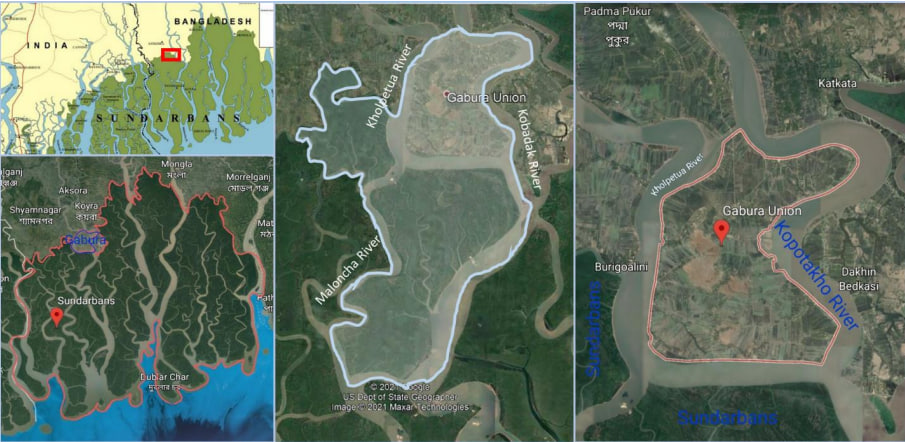
\includegraphics[width=0.5\textwidth]{gabura.jpg}
\caption{Caption of the figure}
\label{fig:gabura}
\end{figure}


\section{ Materials and methods}
%%\label{}
\subsection{Study Area and SES Components}
This area involves multiple agents of different professions associated with the biodiversity of this region.With the variation of parameters affiliated with this socio-economic system,we can further simulate our measures to be taken with regard to the reference of past data giving input to our system.
\subsubsection{Study Area Description}
The study area involves Sunadarbans(Fig.~\ref{fig:gabura}), which is the the world's largest mangrove forest.Our study is specifically focused on Gabura union under Shayamnagar upazilla of Satkhira District.\cite{sweety2022agent}.Mangrove area provides essential livelihood and ensures environmental protection during natural calamities to the coastal areas and the people residing there.The mangrove 
forest (Sundarbans) covers an area over 6,017 km\textsuperscript{2} in Bangladesh of its total area of about 10,000 km\textsuperscript{2}.The several natural elements of the Mangrove area are contributing to the enrichment of its diversity and making the involvement of diversified community fitting into this livelihood system .
\subsubsection{SES Components and Agents}
%%Golpata
Golpata(\textit{Nipa fruticans}),being one of the most abundant species around the mangrove areas,constitute a significant part in the livelihood of mangrove region.They provide economic growth having a variety of using as raw material\cite{jahan2006characterization}. This palm tree lacks a trunk and has tall, upright leaves and a dense root system. It thrives in riverbanks and streams that have a moderate to high salt concentration. It is prevalent in the southern regions of Bangladesh, specifically in Patuakhali, Bagerhat, Khulna, and Satkhira.However.the amount and extent of Golpata are shrinking with time making a threat to the coastal areas population in regard of their existence and income source\cite{financialexpress2020sundarbans}.Golpata palm fronds are used to make roofs, headgear, containers, shade devices, and floor coverings. Palm inflorescence sap may be used to produce vinegar, alcohol, and brown sugar. Edible seed endosperms that are not fully developed are consumable. Annually, a total of 2,100 metric tons of Sundarbans Golpata leaves are collected, providing employment for a workforce of 19,000 individuals. The region's economy is highly dependent on this renewable resource, particularly for its inhabitants who depend on forests \cite{mongabay2020}\cite{banglapedia2021}.Golpata is endangered for both natural and anthropogenic reasons. The population of Golpata has been diminished due to cyclones, elevated salt concentrations, overharvesting, and the degradation of its habitat. The diminishment of this resource poses a risk to the economic and survival needs of the indigenous population who depend on it \cite{mongabay2020}.Ensuring the sustainable protection and management of Golpata necessitates much exertion. In order to guarantee its availability, local non-governmental organizations (NGOs) and research institutes are enhancing their management techniques and cultivating Golpata in specialized nurseries. To save this crucial resource for future generations, it is imperative to implement effective conservation measures, such as sustainable harvesting and habitat restoration\cite{mongabay2020}.\vspace{0.5cm}

%%Fishing
Approximately 1,400 km\textsuperscript{2} make up the World Heritage Site, of which 490 km² are covered by water. A sizable portion of the population depends on fishing, and the Sundarbans' catch fisheries are regarded as the foundation of the SRF economy. 
Since the 1970s, the Sundarbans mangroves have been gradually deteriorating. Because there is less freshwater entering their ecosystem during the dry season, their ecology is altering. Illegal hunting and agricultural encroachment are more issues. However, the Sundarbans' fisheries face a number of challenging issues that affect biodiversity, sustainability, and the way of life for fish resources and fishermen. These issues include pollution, indiscriminate shrimp seed collection, illegal fishing, a lack of post-harvest and other infrastructure, and natural disasters like cyclonic waves.The increased demand for natural shrimp seed, which performs better than hatchery seed, is a direct outcome of the increased shrimp farming along Bangladesh's coast. As a result, there is currently extreme pressure on shrimp fry collecting from Sundarbans water, which is a serious worry. Notwithstanding these issues, there is a considerable chance that the fisheries of the Sundarbans will grow in tandem with interior capture and coastal aquaculture\cite{book}.Fishes of the Sundarbans represent 322 species belonging to 217 genera, 96 families and 22 orders 
117\cite{article}.\vspace{0.5cm}

Agriculture is a significant means of subsistence that has been present in mangrove regions up to now.The agriculture in the Sundarbans is significantly influenced by the unique natural characteristics of the region as well as social factors. The area, which shares borders with both Bangladesh and India, is distinguished by tidal surges, frequent cyclones, and increasing soil salinity, all of which pose significant challenges to traditional agricultural practices. The aftermath of events like Cyclone Aila in 2009 has resulted in persistent consequences, such as the formation of salt deposits on agricultural areas that, even after a decade, have not fully regenerated. Numerous farmers have been compelled to abandon their agricultural lands, thereby prompting their migration to urban areas in pursuit of alternative means of livelihood.Farmers in the Sundarbans are utilizing innovative agricultural practices to adjust to the challenging weather conditions. Utilizing harvested rainwater for irrigation, integrated agricultural techniques that combine aquaculture and rice farming mitigate the impact of saline water intrusion. Enhancing soil health and productivity may be achieved by activities such as cultivating a variety of crops, using dry straw as mulch, and shaping the ground into ridges and furrows. However, the move to shrimp farming has led to significant environmental degradation and financial losses for some farmers due to its high profitability. In order to ensure the enduring viability of farming in this fragile ecosystem, local non-governmental organizations (NGOs) and academic institutions are making efforts to revive traditional agricultural knowledge and promote sustainable farming methods\cite{mongabay2020shrimp}\cite{mongabay2020salt}\cite{mongabay2020caught}\cite{engage4sundarbans2020}.\vspace{0.5cm}

Agent-Based Models (ABM) consist of agents, which are the primary entities defined by qualities and attributes. These agents adhere to pre-established rules or behaviors that govern their interactions within a certain environment. These agents possess dynamic states that undergo changes over time as a result of their interactions and decision-making processes, which can vary from basic if-then principles to intricate algorithms. Agents has the ability to modify their actions based on their experiences, therefore adapting and acquiring new information. The environment exerts a significant impact on human activities and interactions, albeit it is not directly involved. This modeling methodology is utilized in several disciplines, including as epidemiology to simulate the propagation of diseases, economics to analyze market dynamics, and social sciences to investigate social phenomena\cite{railsback2019agent}\cite{bonabeau2002agent}\cite{macal2010tutorial}

This study use simulation to investigate the relationships among crucial groups that depend on mangrove ecosystems, including both individual and collective participants. The corresponding authorities and decision makers control these operations when relevant steps are needed. Hence, the study incorporates Bawalis, Fishers, and Farmers as the main livelihood groups,assigned as agents in the Agent-Based Model (ABM).
\vspace{.5cm}

\textit{Livelihood Agents}
\begin{itemize} 
        \item Bawalis  
        \item Fishers - Types of Fishers:
        \begin{itemize}
            \item Mangrove Fishers - Operate within the mangrove ecosystem.
            \item Household Fishers - Engage in small-scale fishing near their homes.
        \end{itemize}
        \item Farmers
    \end{itemize}
    
These agents make interaction with all those natural components stated beforehand with some specified rules defined in our model.The whole simulation criteria are also scaled by the law enforcing agencies and concerned authorities with their steps taken in respective necessities.
%%Livelihood Description
%%Agents 
% Bawali, Mangrove_Fisher, Household_Fisher, Farmer 


%%------------Anik --------%%
%%Write down the rules and the equations related to these livelihood systems.And describe the model
\subsection{Model and Method}


The aforementioned agents each perform specific actions based on the current condition of the environment. Often these actions alter a certain aspect of the surrounding, thereby affecting the subsequent actions of other agents. In this way, the model captures the interactions among the agents and the environment.

Agents are primarily assigned to a particular occupation. Under unfavorable circumstances, however, they are allowed to switch to other occupations as well for a certain period of time.

\textit{Golpata} (\textit{Nypa fruticans}) forms a major part of the flora of the Sundarbans. A certain group of people named \textit{Bawalis} primarily depends on extracting Golpata throughout the year. To prevent the Golpata stock from dwindling abruptly, each \textit{Bawali} is granted permission to extract a certain maximum amount of \textit{Golpata}. Moreover, the own financial condition of the \textit{Bawali} gives rise to an extraction capacity which puts another limit to the actual extraction amount. In case the extraction capacity of a \textit{Bawali} falls below the minimum allowed capacity, he switches to farming in the following year. If the agent’s permitted amount happens to be zero, he is expected not to perform any extraction that year, which in turn leads to a decline in his extraction capacity for the next year. However, a certain portion of the population turns out to be pilferers. They violate these restrictions and extract \textit{Golpata} even if they are not granted to do so. Each year, natural hazards result in a loss of \textit{Golpata} stock, which the authority tries to replenish by enhancing the conservation rate.

Mangrove Fishers and Household Fishers form another salient part of the livelihood in the Sundarbans. A fisher’s financial state together with the expenditure for movement determines the catching capacity of the Mangrove Fishers for that year. The capacity of the Household Fishers, however, is affected by the cost to produce fish in their vicinity. If the capacity falls below zero, the fisherman takes out a loan, which leads to a slight increase in his capacity. Depending on the amount of catching throughout the year, the fisher’s capacity enhances or declines for the subsequent year. If the capacity crosses a certain threshold, the fisher pays back the loan and regains a portion of the catching capacity.

Natural factors, such as, natural hazards, crop productivity of lands, and human factors like financial condition together control the state of farming. Similar to the previously described occupations, a farmer is also assigned a crop production capacity. If it surpasses the minimum required capacity, a certain amount of crop is produced based on the land productivity and natural hazards. Depending on the production amount, the capacity increases or decreases by a certain percentage of the current capacity. Unless the condition is favorable, the farmer takes out loan, leading to a increase in his capacity. He pays back the loan once he regains the required capacity.
\section{ Results and Discussions}

The whole agent based model is characterized by various time dependent and independent parameters.The time dependent parameters can be taken as input as csv files and we can predict the agent based simulation on the basis of previous years' data .Moreover,time independent data and time dependent data both can be taken as input with the slider of simulation.The model depicts a comprehensive analysis of the SES components over time and different strategies taken in favour of management of all these.
\subsection{Different Cases and Outcomes}
Three SES cases are selected to examine system performance and agent behavior within a feasible variable range. These cases focus on the variation in the catching capacity of both types of fishers, crop production capacity of farmers, and the permitted golpata amount for the Bawalis. The model variables that distinguish these cases are listed in Table~\ref{tab:case-scenarios}.

\begin{itemize}
    \item \textbf{Case 1} features a high golpata permit for Bawalis, low catching capacities for both types of fishers, and high crop production capacity.
    \item \textbf{Case 2} includes moderate golpata permits, moderate catching capacities for fishers, and low crop production capacity.
    \item \textbf{Case 3} presents comparatively low golpata permits, high catching capacities for fishers, and moderate crop production capacity.
\end{itemize}

Table~\ref{tab:case-scenarios} summarizes the variable values for each case, showing the metrics for golpata permits, catching capacities, and crop production.

Additionally, global variables affecting agent behavior---some positively, others negatively---also play a role in determining how the ecosystem responds under different conditions.

\begin{table}[h!]
\centering
\scriptsize  % Adjust font size
\setlength{\tabcolsep}{3pt}  % Reduce column padding
\renewcommand{\arraystretch}{1.1}  % Adjust row height
\begin{tabular}{|c|l|c|}
\hline
\textbf{Case Number} & \textbf{Variable}                  & \textbf{Value (Metric ton)} \\ \hline
\multirow{4}{*}{Case 1} & golpata\_permit                   & 125                        \\ \cline{2-3} 
                       & catching\_capacity\_M             & 2.3                        \\ \cline{2-3} 
                       & catching\_capacity\_H             & 2.3                        \\ \cline{2-3} 
                       & crop\_production\_capacity        & 5                          \\ \hline
\multirow{4}{*}{Case 2} & golpata\_permit                   & 120                        \\ \cline{2-3} 
                       & catching\_capacity\_M             & 2.4                        \\ \cline{2-3} 
                       & catching\_capacity\_H             & 2.4                        \\ \cline{2-3} 
                       & crop\_production\_capacity        & 4.75                       \\ \hline
\multirow{4}{*}{Case 3} & golpata\_permit                   & 115                        \\ \cline{2-3} 
                       & catching\_capacity\_M             & 2.5                        \\ \cline{2-3} 
                       & catching\_capacity\_H             & 2.5                        \\ \cline{2-3} 
                       & crop\_production\_capacity        & 4.5                        \\ \hline
\end{tabular}
\caption{Variable values for the three cases}
\label{tab:case-scenarios}
\end{table}
Three scenarios are chosen to simulate each case:
\begin{itemize}
    \item \textbf{Favorable scenario:} This scenario considers the highest values of global variables that have a positive impact and the lowest values for those with a negative impact, as configured in the MESA framework sliders.
    \item \textbf{Moderate scenario:} This scenario assumes moderate values for all global variables.
    \item \textbf{Critical scenario:} This scenario selects the highest values for global variables with a negative impact and the lowest values for those with a positive impact.
\end{itemize}

The global variable values for each scenario are as follows:

\begin{itemize}
    \item \textbf{Global Variable Values for the Favorable Scenario:}
    \begin{itemize}
        \item Movement cost for Bawali: 10 metric tons
        \item Golpata conservation growth rate: 150 metric tons
        \item Golpata natural growth rate: 75 metric tons
        \item Natural hazard loss: 50 metric tons
        \item Ice cost: 0.25 metric tons
        \item Movement cost for Fishermen\_M: 0.25 metric tons
        \item Production cost of fish: 0.25 metric tons
        \item Natural hazard loss (crops): 0.5 metric tons
        \item Fertilizer cost: 0.5 metric tons
        \item Extraction control efficiency: 4
        \item Regulatory efficiency: 2
    \end{itemize}

    \item \textbf{Global Variable Values for the Moderate Scenario:}
    \begin{itemize}
        \item Movement cost for Bawali: 14.75 metric tons
        \item Golpata conservation growth rate: 125 metric tons
        \item Golpata natural growth rate: 62.5 metric tons
        \item Natural hazard loss: 75 metric tons
        \item Ice cost: 0.375 metric tons
        \item Movement cost for Fishermen\_M: 0.375 metric tons
        \item Production cost of fish: 0.5 metric tons
        \item Natural hazard loss (crops): 0.75 metric tons
        \item Fertilizer cost: 0.75 metric tons
        \item Extraction control efficiency: 3
        \item Regulatory efficiency: 1.5
    \end{itemize}

    \item \textbf{Global Variable Values for the Critical Scenario:}
    \begin{itemize}
        \item Movement cost for Bawali: 20 metric tons
        \item Golpata conservation growth rate: 100 metric tons
        \item Golpata natural growth rate: 50 metric tons
        \item Natural hazard loss: 100 metric tons
        \item Ice cost: 0.5 metric tons
        \item Movement cost for Fishermen\_M: 0.5 metric tons
        \item Production cost of fish: 0.75 metric tons
        \item Natural hazard loss (crops): 1 metric ton
        \item Fertilizer cost: 1 metric ton
        \item Extraction control efficiency: 2
        \item Regulatory efficiency: 1
    \end{itemize}
\end{itemize}
\subsection{Behaviour of Agents in Different Scenarios}
\subsubsection{Favourable Condition:}
The figures (2-7) and tables (2-7) illustrate the changes in outcomes associated with the livelihood agents over time, under the given favourable circumstances. We can conduct a comprehensive assessment of these elements over a prolonged period. The X-axis represents each year, and the graphs show data for a maximum of 90 years, giving a thorough overview of long-term trends.

The condition of the "Golpata Stock," which holds enormous importance for the Bawali people, acts as a crucial gauge of resource sustainability. The trends identified in these plots provide essential insights about the resilience and availability of this crucial resource. The plots labelled "Mangrove Fishers in Loan" and "Catching Capacity Mangrove" are essential for understanding the behaviours and results of mangrove fishers. These graphs offer valuable information on how these communities manage financial borrowing and resource allocation under favourable circumstances.
The plots labelled "Household Fishers in Loan" and "Catching Capacity Household" are of enormous significance to household fishermen. This data illustrates the changing patterns within these communities, particularly the fluctuations in loan acquisition and resource capacity over time. Furthermore, the plots headed "Farmers in Loan" and "Crop Production Capacity" are crucial in illustrating farmers' adaptive methods and their efficient use of resources.
To do a thorough examination, statistical measures have been calculated for each individual case, mirroring the approach used for the moderate conditions. These measurements facilitate a direct and accurate comparison of the three scenarios, allowing us to examine similarities and differences with precision. The data not only reinforces the observed patterns in the plots but also ensures a full and lucid explanation of the comparison results for each livelihood agent.\\
% First figure for Bawali
\begin{figure}[htbp]
    \centering
    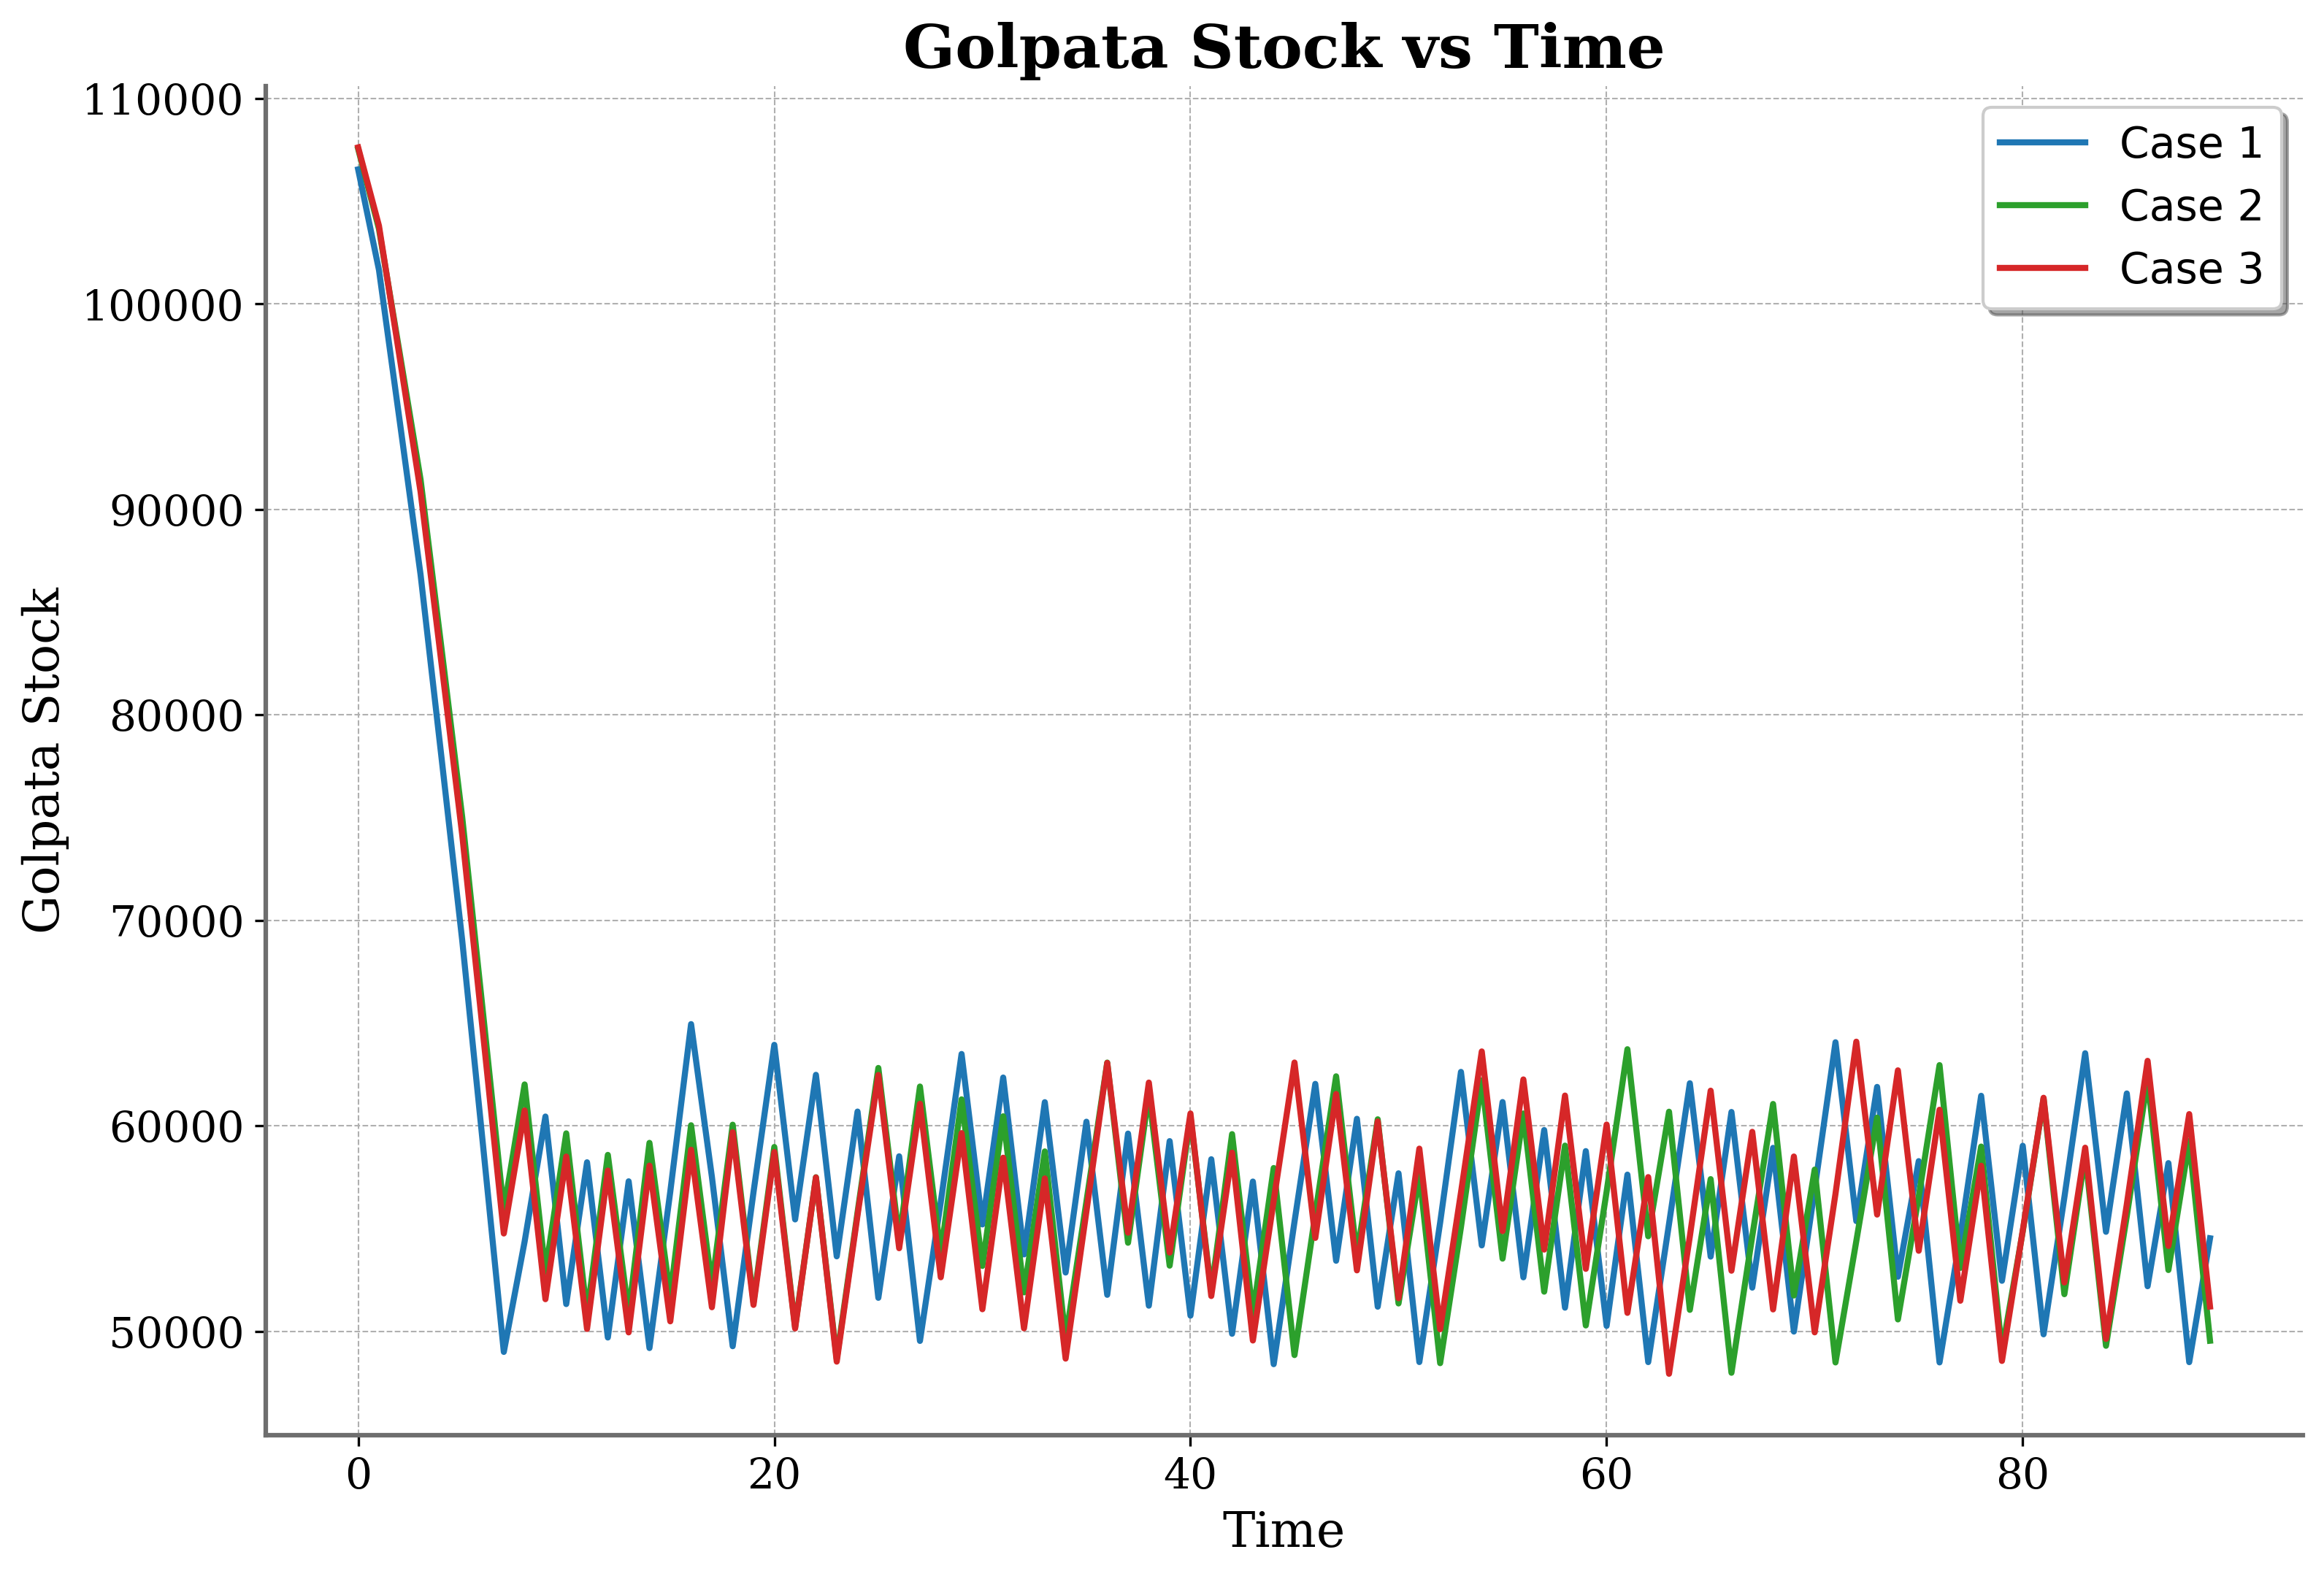
\includegraphics[width=0.4\textwidth]{graph_all/plots_fav/golpata_stock_vs_time.png}
    \caption{Golpata Stock vs Time for Bawali}
    \label{fig:bawali}
\end{figure}
\begin{table}[htbp]
    \centering
    \resizebox{0.4\textwidth}{!}{ % Adjust the 0.9 to control the table size
    \begin{tabular}{lccc}
        \toprule
        \textbf{Statistic} & \textbf{Case 1} & \textbf{Case 2} & \textbf{Case 3} \\
        \midrule
        Mean & 58184.1 & 58410.8 & 58503.2 \\
        Median & 56787.2 & 56439.4 & 56724.7 \\
        Min & 48404.4 & 47986 & 47936.4 \\
        Max & 106550 & 107545 & 107621 \\
        Range & 58145.9 & 59559.5 & 59685 \\
        Standard Deviation & 10099.8 & 10733.6 & 10654.8 \\
        Variance & 1e+08 & 1.2e+08 & 1.1e+08 \\
        Interquartile Range & 8358.95 & 8523.76 & 8829.49 \\
        Skewness & 2.87376 & 2.86295 & 2.87588 \\
        Kurtosis & 9.78466 & 9.11898 & 9.28546 \\
        First Quartile & 52264.4 & 51937.3 & 51885.5 \\
        Third Quartile & 60623.4 & 60461.1 & 60715 \\
        MAD & 4240.44 & 4230.72 & 4217.94 \\
        Coefficient of Variation & 0.17358 & 0.18376 & 0.18212 \\
        Mode & 48404.4 & 47986 & 47936.4 \\
        \bottomrule
    \end{tabular}
    }
    \caption{Golpata Stock - Statistical Analysis}
\end{table}
When examining Golpata stock in favourable conditions (Figure 2 and Table 2), a same pattern emerges in all three scenarios: an abrupt decrease initially, followed by a stabilisation phase with periodic fluctuations. The mean and median values across cases are tightly correlated, suggesting comparable average stock levels during the stabilisation phase. Nevertheless, Case 3 demonstrates a significantly greater degree of variability, as evidenced by its range, standard deviation, and interquartile range, indicating more significant changes. The skewness and kurtosis values suggest that the distribution of cases is skewed to the right and has a high peak, indicating that the system is highly responsive to early shocks and contains a significant number of extreme values. The coefficient of variation remains constant at approximately 0.18 for all cases, indicating continuous relative variability. However, the data shows that while stock levels stabilise, there are still ongoing oscillations, particularly in Case 3. Ultimately, the system moves towards stability following early disturbances. However, the observed oscillations indicate the need for cautious management to prevent excessive extraction of resources, particularly in cases resembling Case 3, where variations are more pronounced.\\
% Second figure for Mangrove Fishermen
\begin{figure}[htbp]
    \centering
    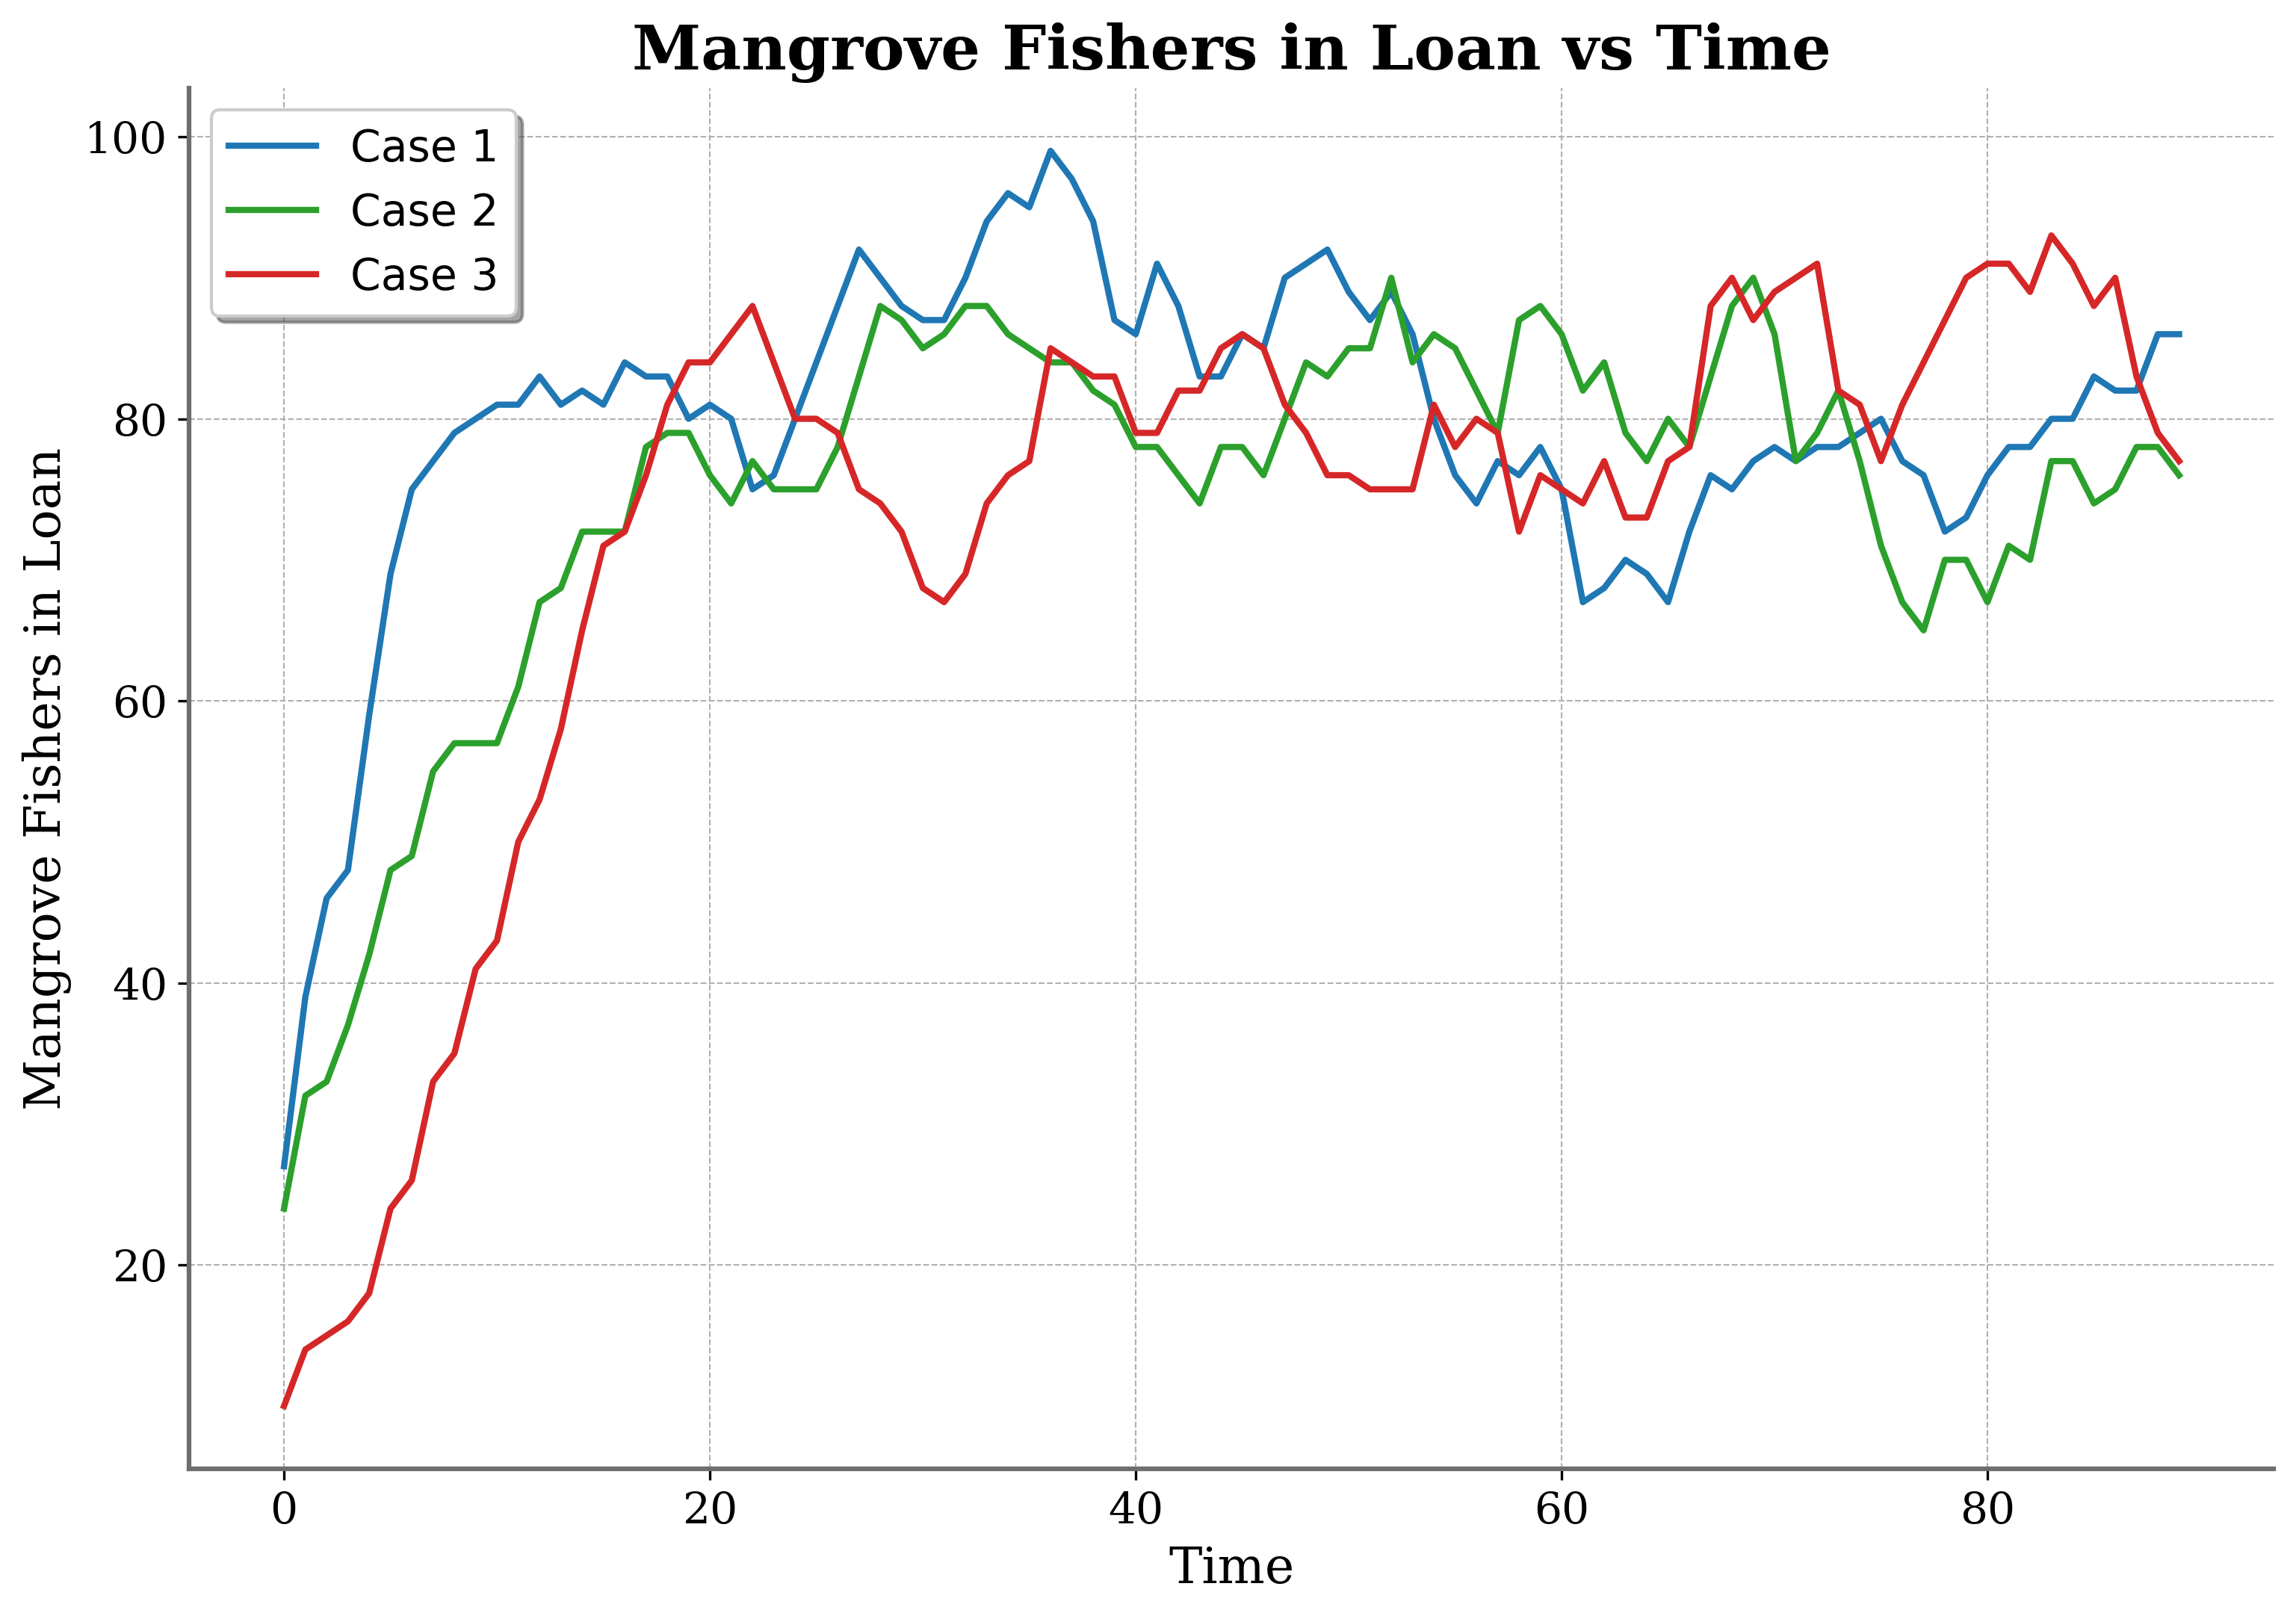
\includegraphics[width=0.4\textwidth]{graph_all/plots_fav/mangrove_fishers_in_loan_vs_time.png}
    \caption{Mangrove Fishers in Loan vs Time}
    \label{fig:mangrove_loan}
\end{figure}
% Mangrove Fishers in Loan - Statistical Analysis
\begin{table}[htbp]
    \centering
    \resizebox{0.4\textwidth}{!}{ % Adjust the 0.9 to control the table size
    \begin{tabular}{lccc}
        \toprule
        \textbf{Statistic} & \textbf{Case 1} & \textbf{Case 2} & \textbf{Case 3} \\
        \midrule
        Mean & 79.5556 & 74.7333 & 72.7778 \\
        Median & 80 & 78 & 79 \\
        Min & 27 & 24 & 10 \\
        Max & 99 & 90 & 93 \\
        Range & 72 & 66 & 83 \\
        Standard Deviation & 11.4206 & 13.3861 & 19.8855 \\
        Variance & 130.429 & 179.187 & 395.433 \\
        Interquartile Range & 10 & 12 & 11 \\
        Skewness & -1.94443 & -1.85024 & -1.86996 \\
        Kurtosis & 6.02364 & 3.41867 & 2.58969 \\
        First Quartile & 76 & 72 & 73 \\
        Third Quartile & 86 & 84 & 84 \\
        MAD & 5 & 6 & 5.5 \\
        Coefficient of Variation & 0.14355 & 0.17912 & 0.27324 \\
        Mode & 80 & 78 & 79 \\
        \bottomrule
    \end{tabular}
    }
    \caption{Mangrove Fishers in Loan - Statistical Analysis}
\end{table}
The time-series analysis of Mangrove Fishers in Loan (Figure 3 and Table 3) shows a steady increase in loan participation among fishers in Scenario 1, followed by a period of fluctuation. Cases 2 and 3 show more significant changes, with Case 3 showing the highest level of variability. The data suggests that Case 1 offers a more stable setting for mangrove fishers, with continuous loan participation and reduced variability. However, Cases 2 and 3, particularly Case 3, show increased unpredictability and volatility in fisher behavior, possibly due to external factors like economic circumstances, regulatory modifications, or environmental difficulties. These observations highlight the need for focused measures to stabilize fishermen's involvement in situations prone to fluctuations.\\
% Third figure for Catching Capacity Mangrove
\begin{figure}[htbp]
    \centering
    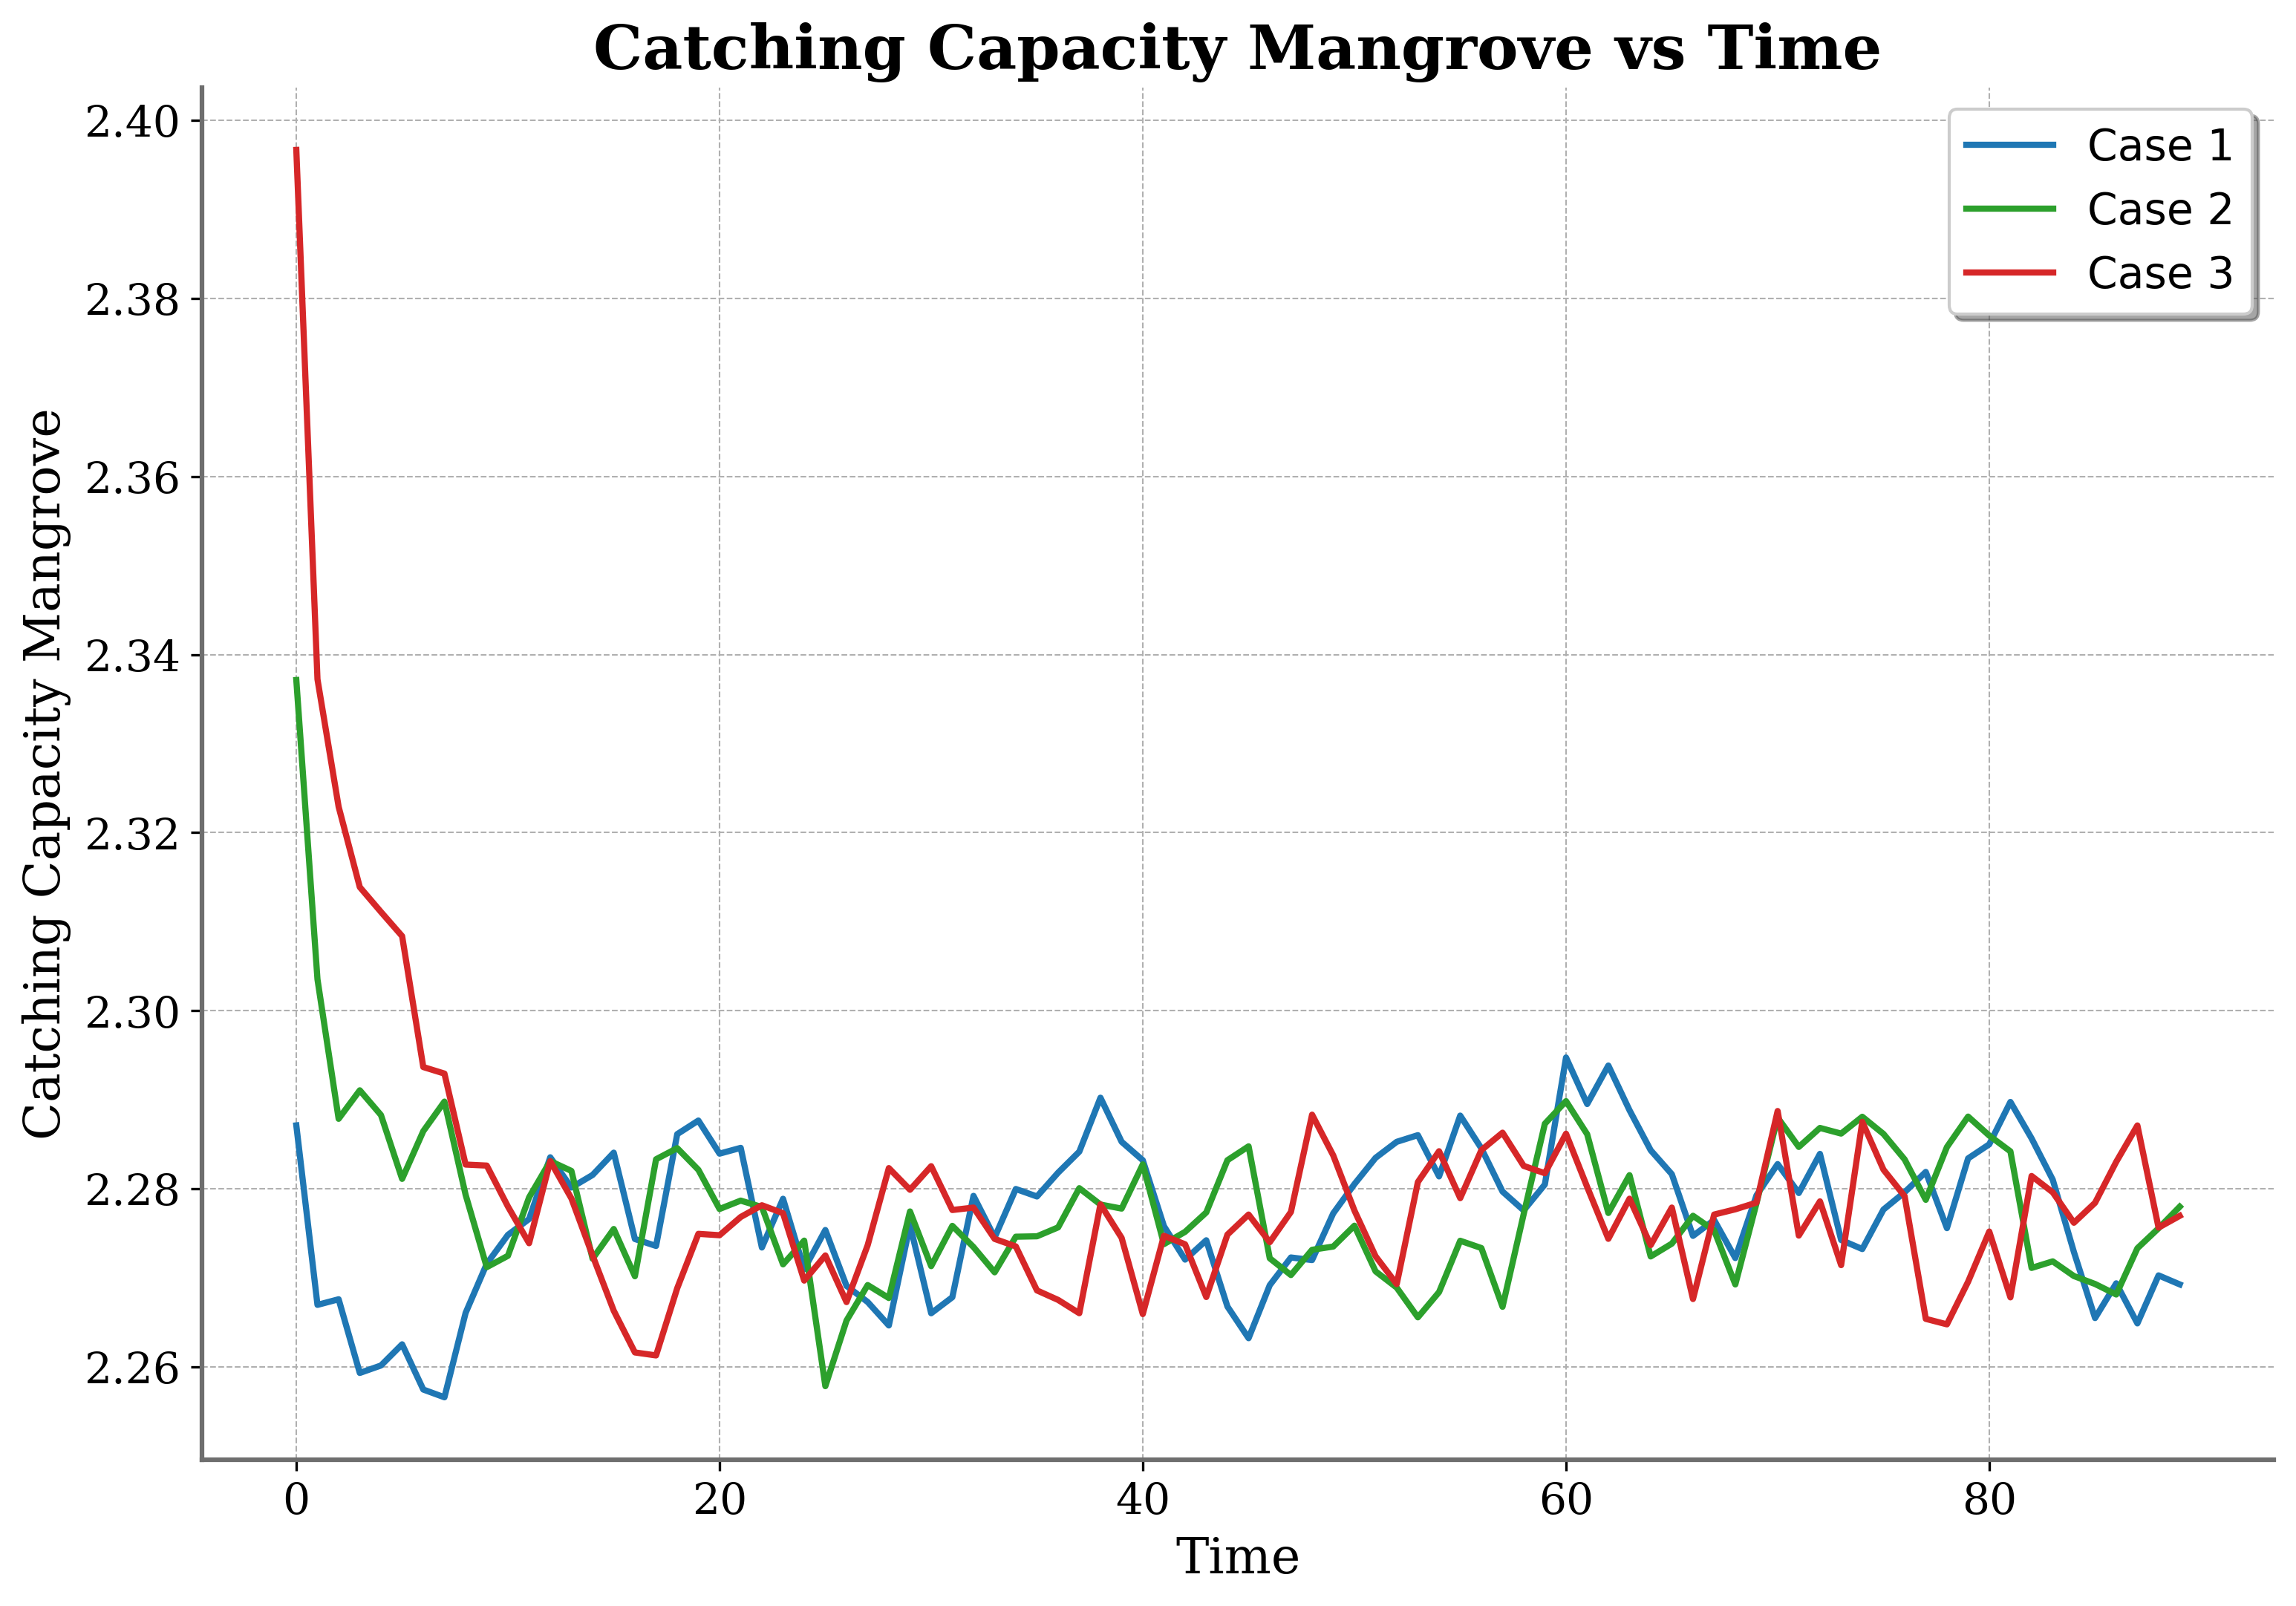
\includegraphics[width=0.4\textwidth]{graph_all/plots_fav/catching_capacity_mangrove_vs_time.png}
    \caption{Catching Capacity Mangrove vs Time}
    \label{fig:catching_mangrove}
\end{figure}

\begin{table}[htbp]
    \centering
    \resizebox{0.4\textwidth}{!}{
    \begin{tabular}{lccc}
        \toprule
        \textbf{Statistic} & \textbf{Case 1} & \textbf{Case 2} & \textbf{Case 3} \\
        \midrule
        Mean & 2.27696 & 2.27833 & 2.28032 \\
        Median & 2.27765 & 2.27725 & 2.27762 \\
        Min & 2.25662 & 2.25787 & 2.26132 \\
        Max & 2.29477 & 2.33714 & 2.39665 \\
        Range & 0.03814 & 0.07927 & 0.13533 \\
        Standard Deviation & 0.00839 & 0.00968 & 0.0172 \\
        Variance & 7.04e-05 & 9.37e-05 & 0.0003 \\
        Interquartile Range & 0.01183 & 0.01106 & 0.00881 \\
        Skewness & -0.30521 & 2.59163 & 4.17231 \\
        Kurtosis & -0.45016 & 13.6465 & 23.0105 \\
        First Quartile & 2.27171 & 2.27228 & 2.2737 \\
        Third Quartile & 2.28355 & 2.28334 & 2.28251 \\
        MAD & 0.00598 & 0.0058 & 0.00464 \\
        Coefficient of Variation & 0.00369 & 0.00425 & 0.00754 \\
        Mode & 2.25662 & 2.25787 & 2.26132 \\
        \bottomrule
    \end{tabular}
    }
    \caption{Catching Capacity Mangrove - Statistical Analysis}
\end{table}
The Catching Capacity for Mangrove graph (Figure 4 and Table 4) shows a precipitous decrease in catching ability, followed by a period of stabilization with intermittent variations. Case 1 has the smallest average value, while Cases 2 and 3 have gradually increasing average values. Case 3 has higher variability and dispersion, possibly due to external factors or resource management obstacles. The skewness and kurtosis values show that Case 1 has a more symmetrical distribution, while Cases 2 and 3 have more pronounced fluctuations. The findings suggest that stronger management measures are needed to ensure stability in situations like Case 3, where fishing conditions are more volatile.\\
% Fourth figure for Household Fishers in Loan
\begin{figure}[htbp]
    \centering
    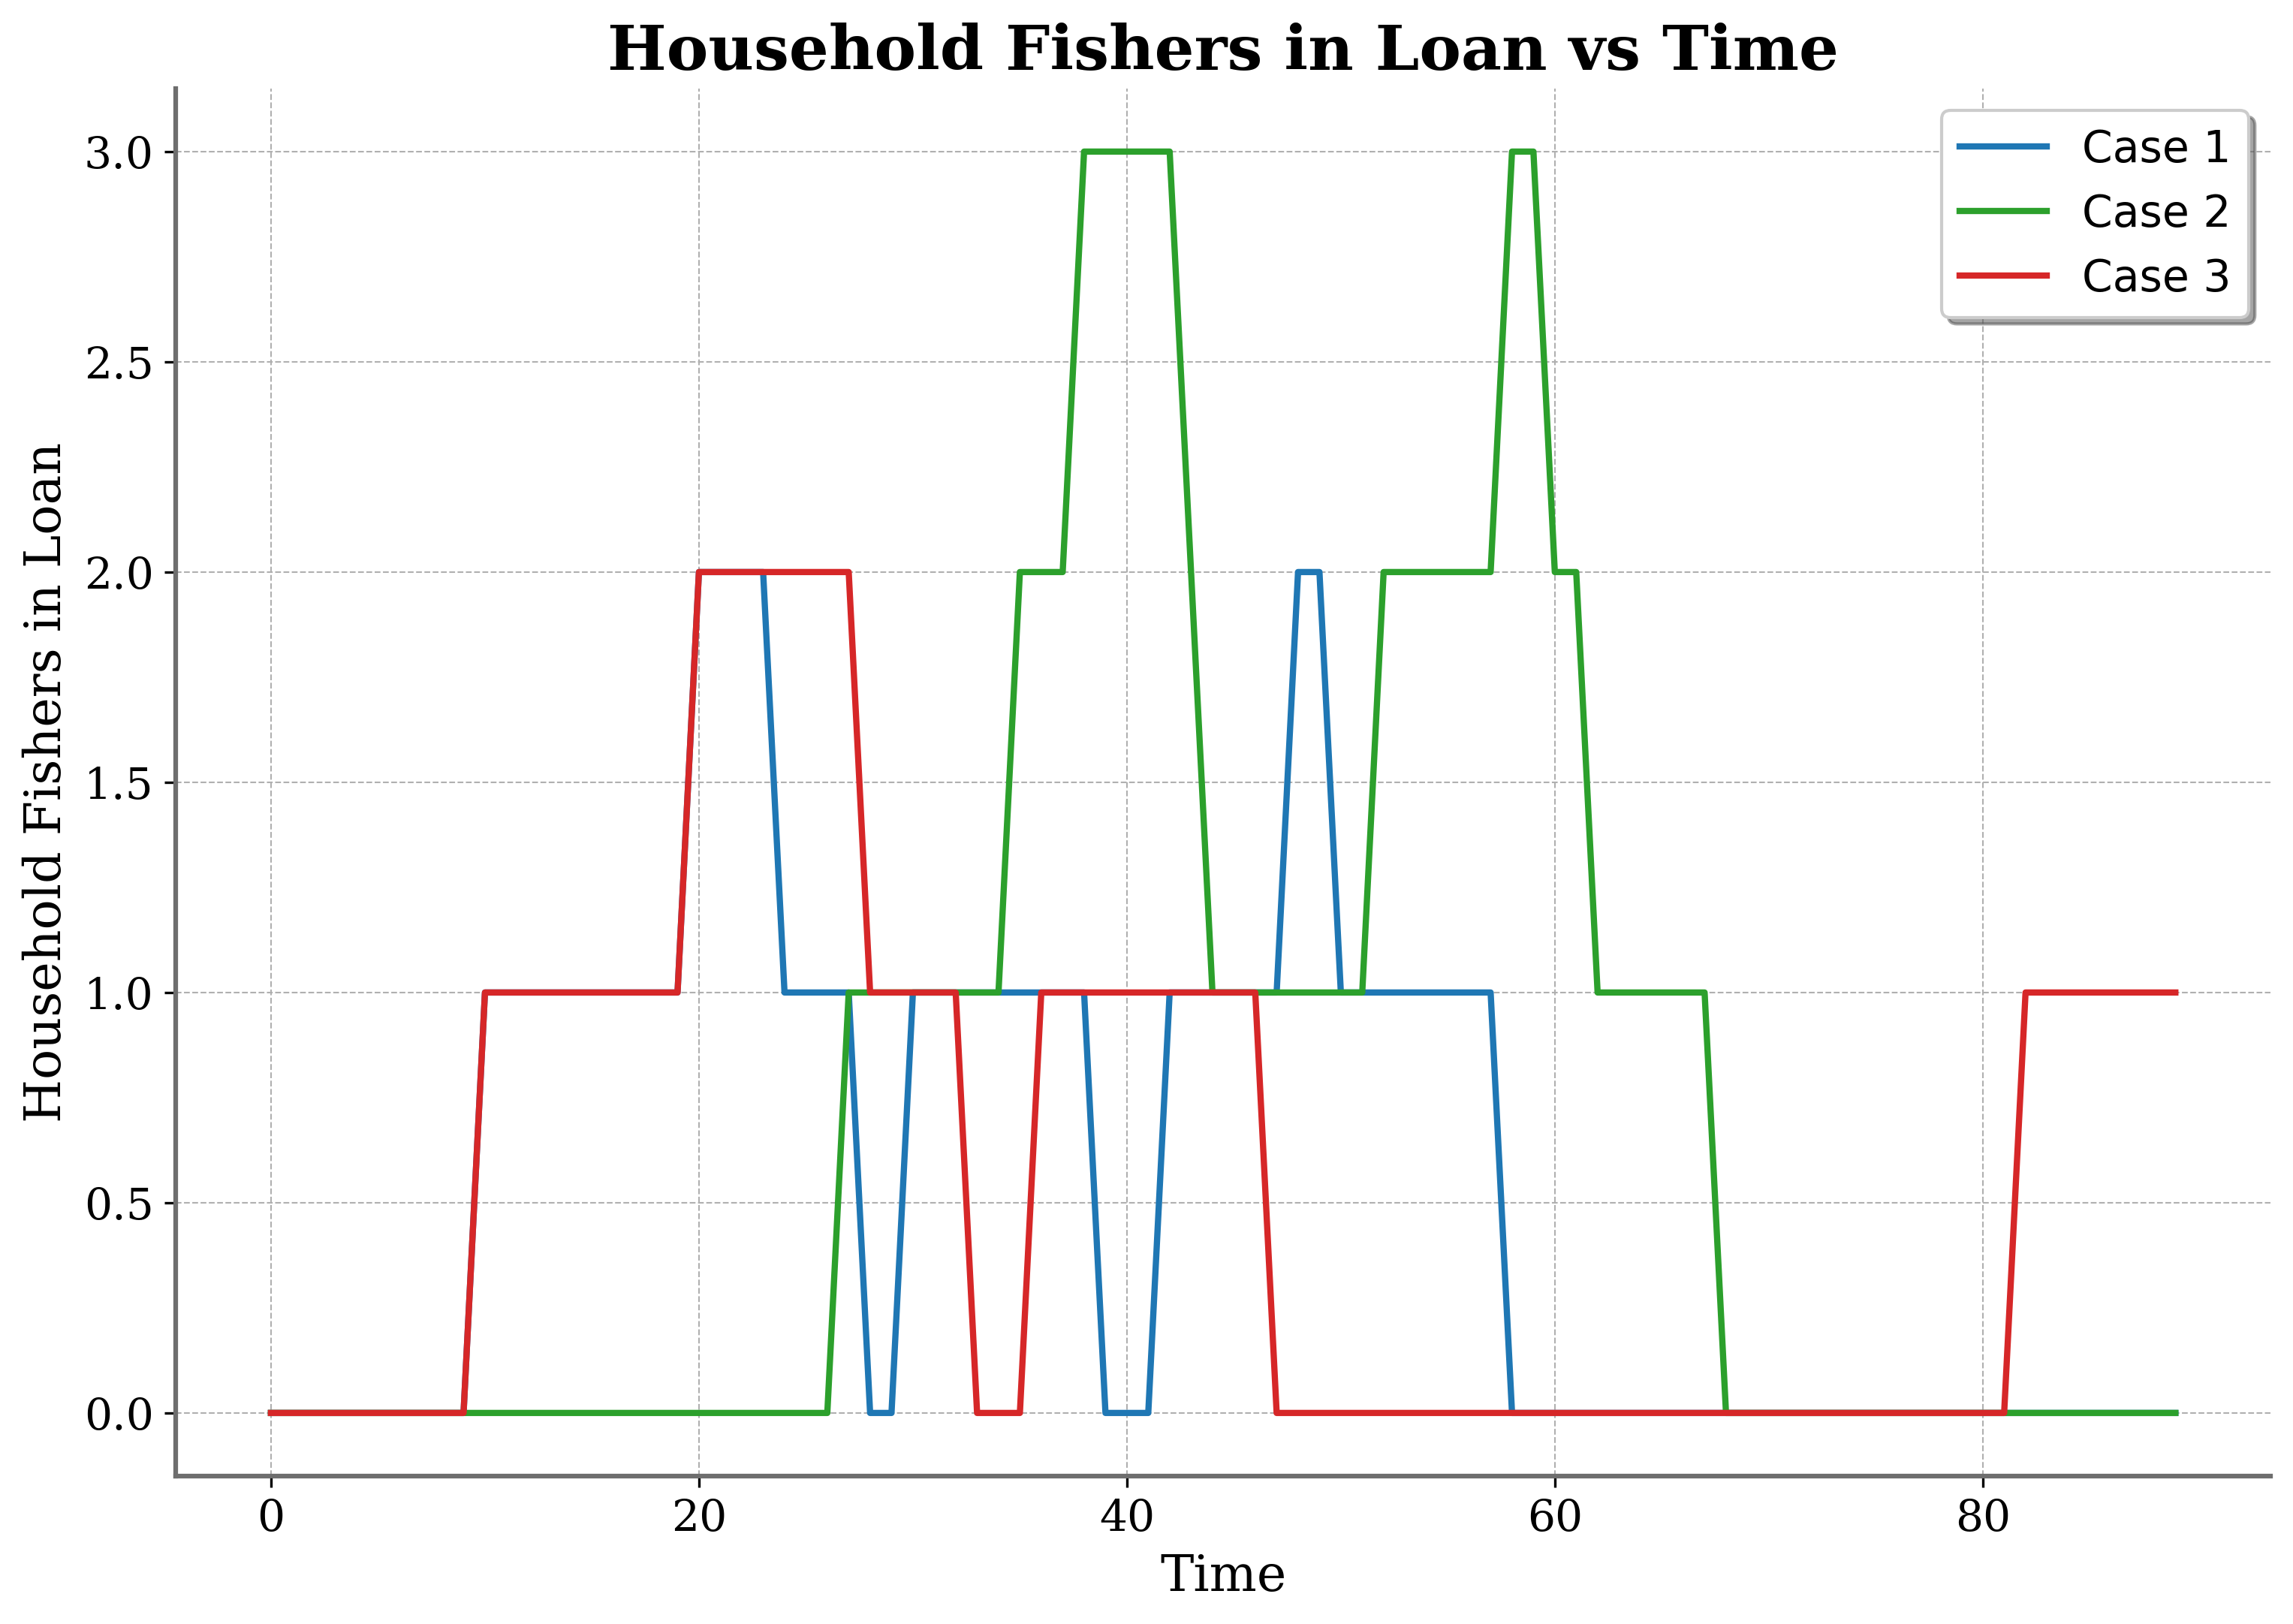
\includegraphics[width=0.4\textwidth]{graph_all/plots_fav/household_fishers_in_loan_vs_time.png}
    \caption{Household Fishers in Loan vs Time}
    \label{fig:household_loan}
\end{figure}
% Household Fishers in Loan - Statistical Analysis
\begin{table}[htbp]
    \centering
    \resizebox{0.4\textwidth}{!}{ % Adjust the 0.9 to control the table size
    \begin{tabular}{lccc}
        \toprule
        \textbf{Statistic} & \textbf{Case 1} & \textbf{Case 2} & \textbf{Case 3} \\
        \midrule
        Mean & 0.544444 & 0.744444 & 0.555556 \\
        Median & 0 & 0 & 0 \\
        Min & 0 & 0 & 0 \\
        Max & 2 & 3 & 2 \\
        Range & 2 & 3 & 2 \\
        Standard Deviation & 0.621 & 0.96641 & 0.65533 \\
        Variance & 0.38564 & 0.93396 & 0.42946 \\
        Interquartile Range & 1 & 1 & 1 \\
        Skewness & 0.68014 & 1.05441 & 0.75733 \\
        Kurtosis & -0.50516 & -0.05425 & -0.49121 \\
        First Quartile & 0 & 0 & 0 \\
        Third Quartile & 1 & 1 & 1 \\
        MAD & 1.14062 & 1.29817 & 1.1796 \\
        Coefficient of Variation & 0 & 0 & 0 \\
        Mode & 0 & 0 & 0 \\
        \bottomrule
    \end{tabular}
    }
    \caption{Household Fishers in Loan - Statistical Analysis}
\end{table}
The study of household fishers' loan participation (Figure 5 and Table 5) shows irregular patterns, with sudden surges and extended periods of inactivity. Case 1 shows a restrained level of involvement, while Cases 2 and 3 show elevated peaks and frequent variations, suggesting increased borrowing susceptibility. Case 2 has the highest standard deviation and variance, indicating greater unpredictability and spread in loan behavior. The mode and median values consistently indicate zero loan participation, with occasional temporary increases. Case 2 has the most extensive dispersion, suggesting a more diverse loan participation scenario. To ensure financial security, governmental initiatives targeting these periods of increased activity are necessary.\\
% Fifth figure for Catching Capacity Household
\begin{figure}[htbp]
    \centering
    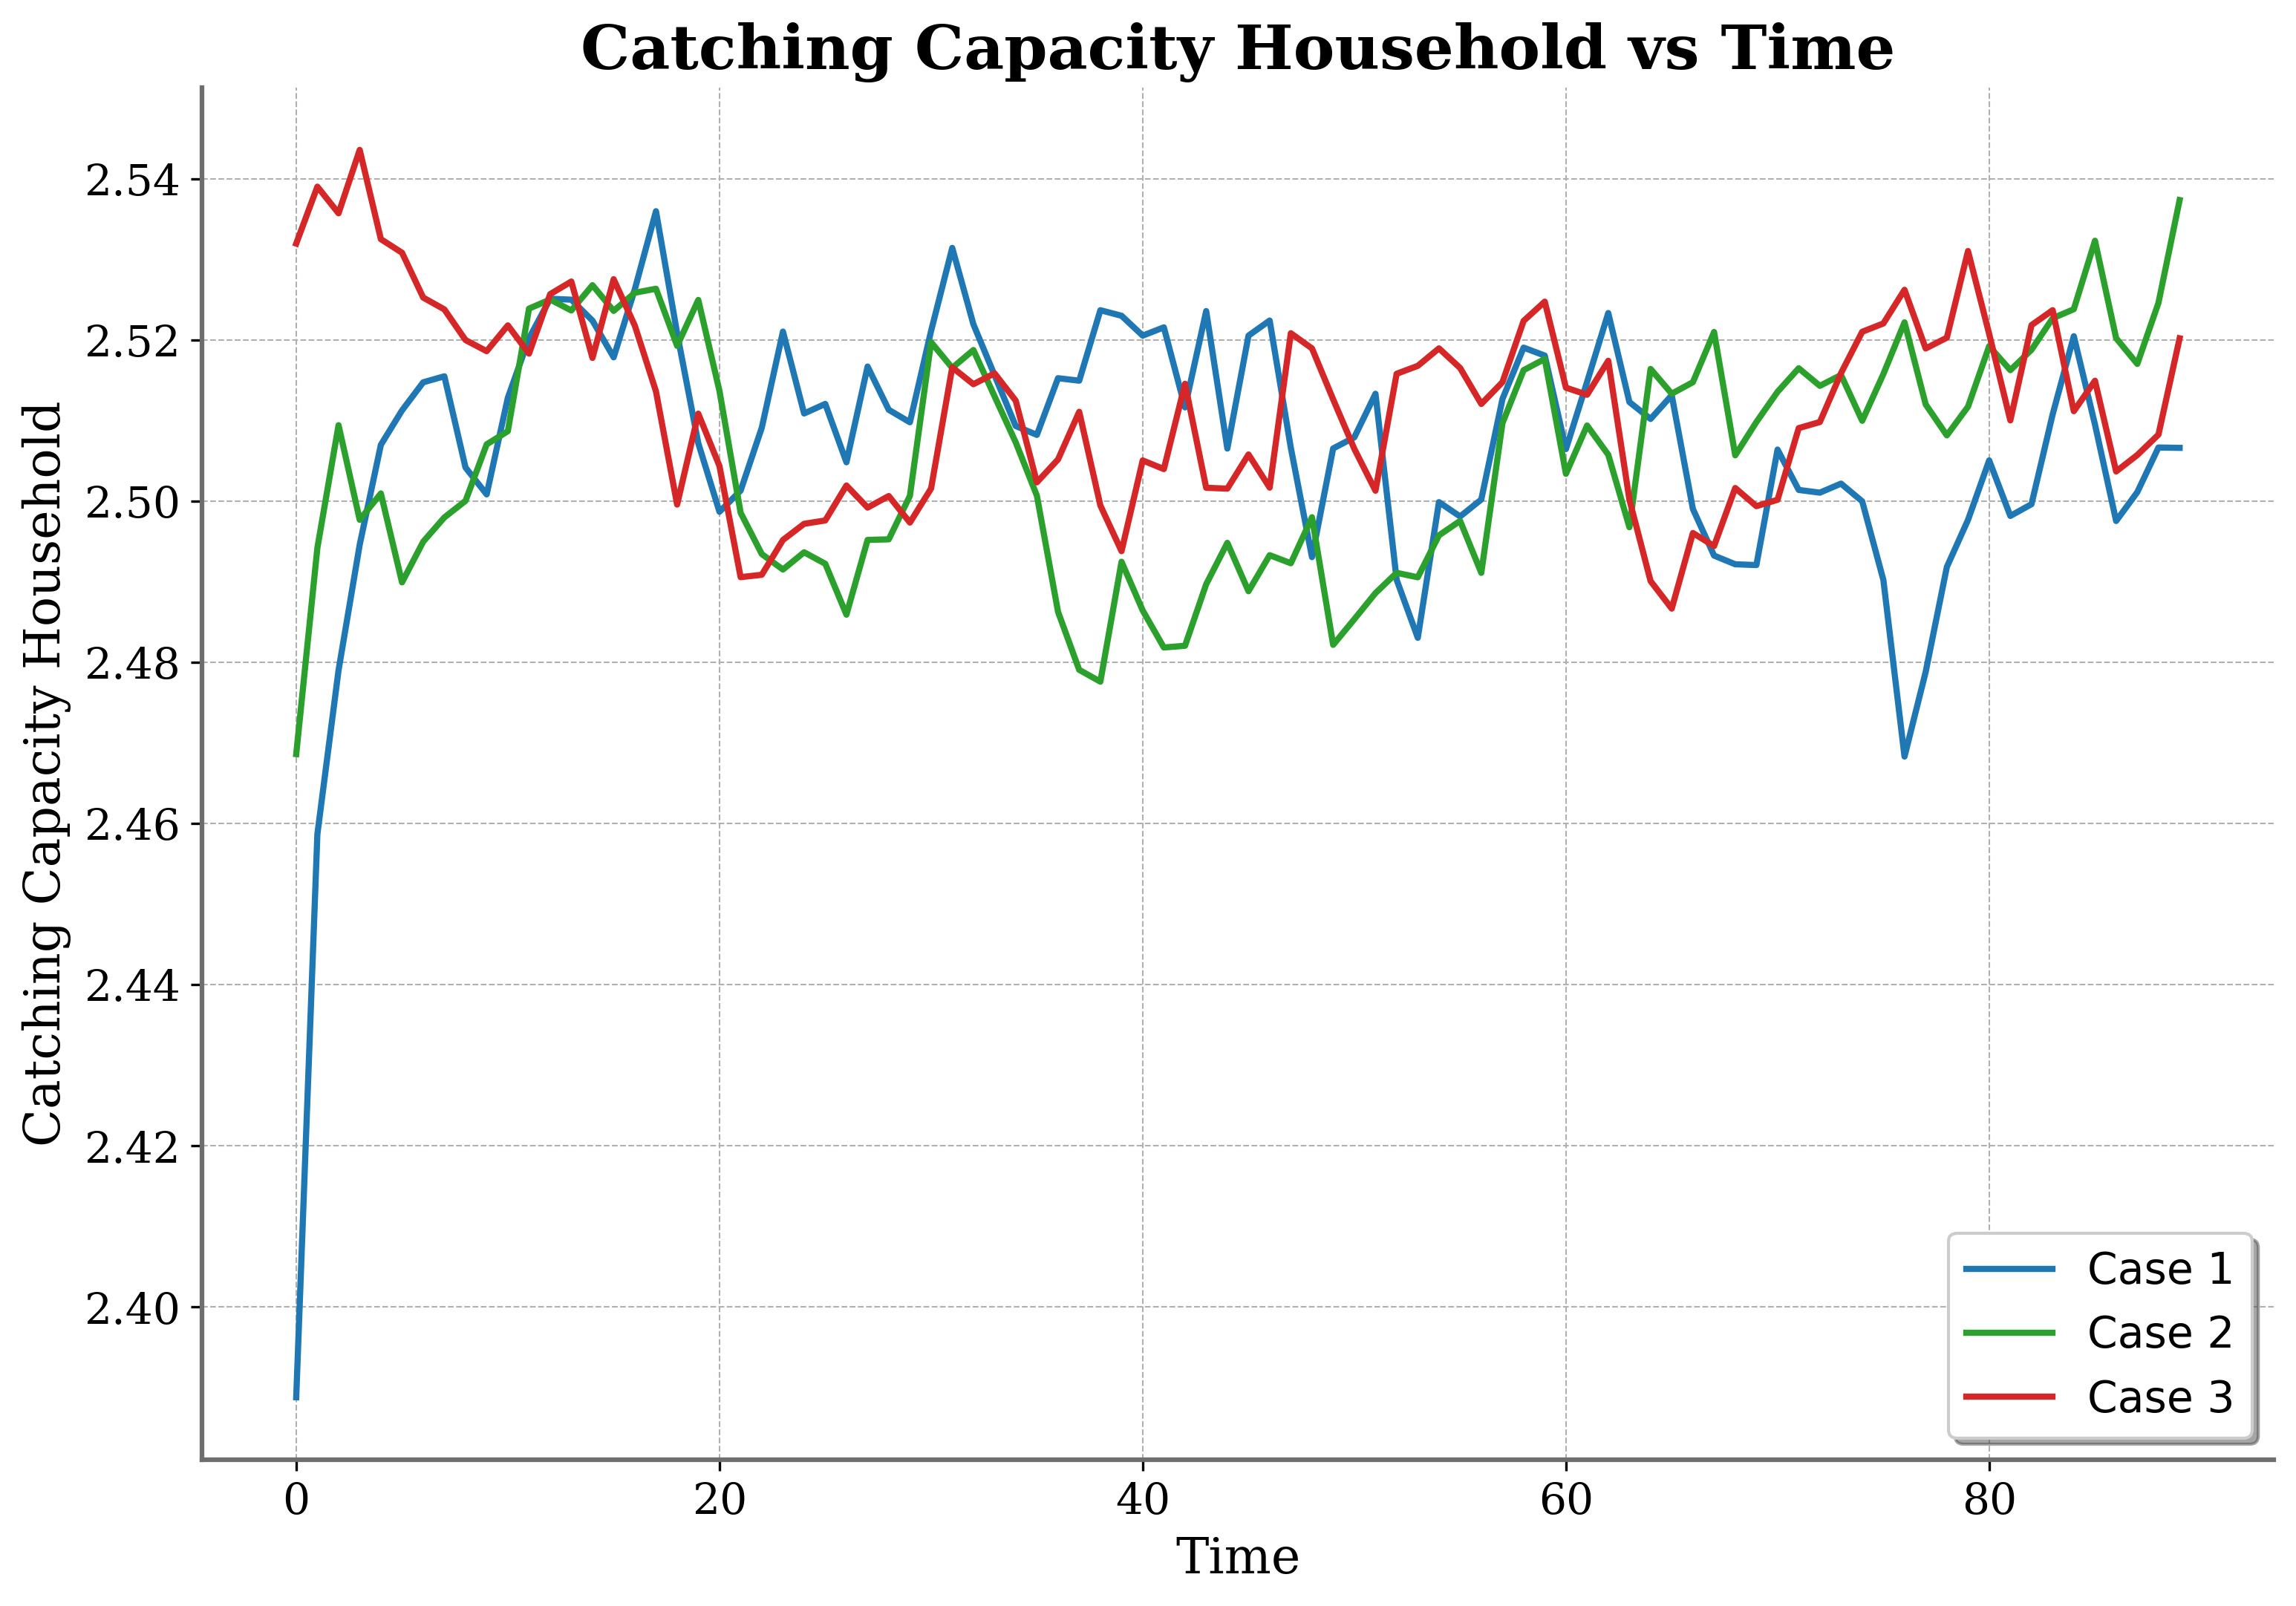
\includegraphics[width=0.4\textwidth]{graph_all/plots_fav/catching_capacity_household_vs_time.png}
    \caption{Catching Capacity Household vs Time}
    \label{fig:catching_household}
\end{figure}
\begin{table}[htbp]
    \centering
    \resizebox{0.4\textwidth}{!}{
    \begin{tabular}{lccc}
        \toprule
        \textbf{Statistic} & \textbf{Case 1} & \textbf{Case 2} & \textbf{Case 3} \\
        \midrule
        Mean & 2.50662 & 2.5056 & 2.51222 \\
        Median & 2.50924 & 2.50775 & 2.51343 \\
        Min & 2.38881 & 2.46863 & 2.48668 \\
        Max & 2.536 & 2.53738 & 2.54361 \\
        Range & 0.14719 & 0.06876 & 0.05692 \\
        Standard Deviation & 0.01822 & 0.01466 & 0.01201 \\
        Variance & 0.00033 & 0.00021 & 0.00014 \\
        Interquartile Range & 0.01753 & 0.02341 & 0.01897 \\
        Skewness & -3.28588 & -0.15918 & 0.12086 \\
        Kurtosis & 18.0593 & -0.84757 & -0.48441 \\
        First Quartile & 2.50005 & 2.49351 & 2.50168 \\
        Third Quartile & 2.51758 & 2.51692 & 2.52065 \\
        MAD & 0.00893 & 0.01223 & 0.0088 \\
        Coefficient of Variation & 0.00727 & 0.00585 & 0.00478 \\
        Mode & 2.38881 & 2.46863 & 2.48668 \\
        \bottomrule
    \end{tabular}
    }
    \caption{Catching Capacity Household - Statistical Analysis}
\end{table}
The Catching Capacity Household study (Figure 6 and Table 6)reveals a consistent increase in catching capacity over time, with Case 3 showing slightly greater levels. Case 1 has greater stability, while Case 2 shows more swings. The average catching capacities are similar in all cases, with Case 3 having the highest value of 2.512. However, Case 1 has a more pronounced negative skewness and lower kurtosis values. Cases 2 and 3 have a more symmetrical distribution but more prominent tails. The mode remains constant in all cases, with Case 3 having the largest central tendency. Overall, Case 1 shows greater stability and consistency, while Cases 2 and 3 have greater capacity but more instability.\\
% Sixth figure for Farmers in Loan
\begin{figure}[htbp]
    \centering
    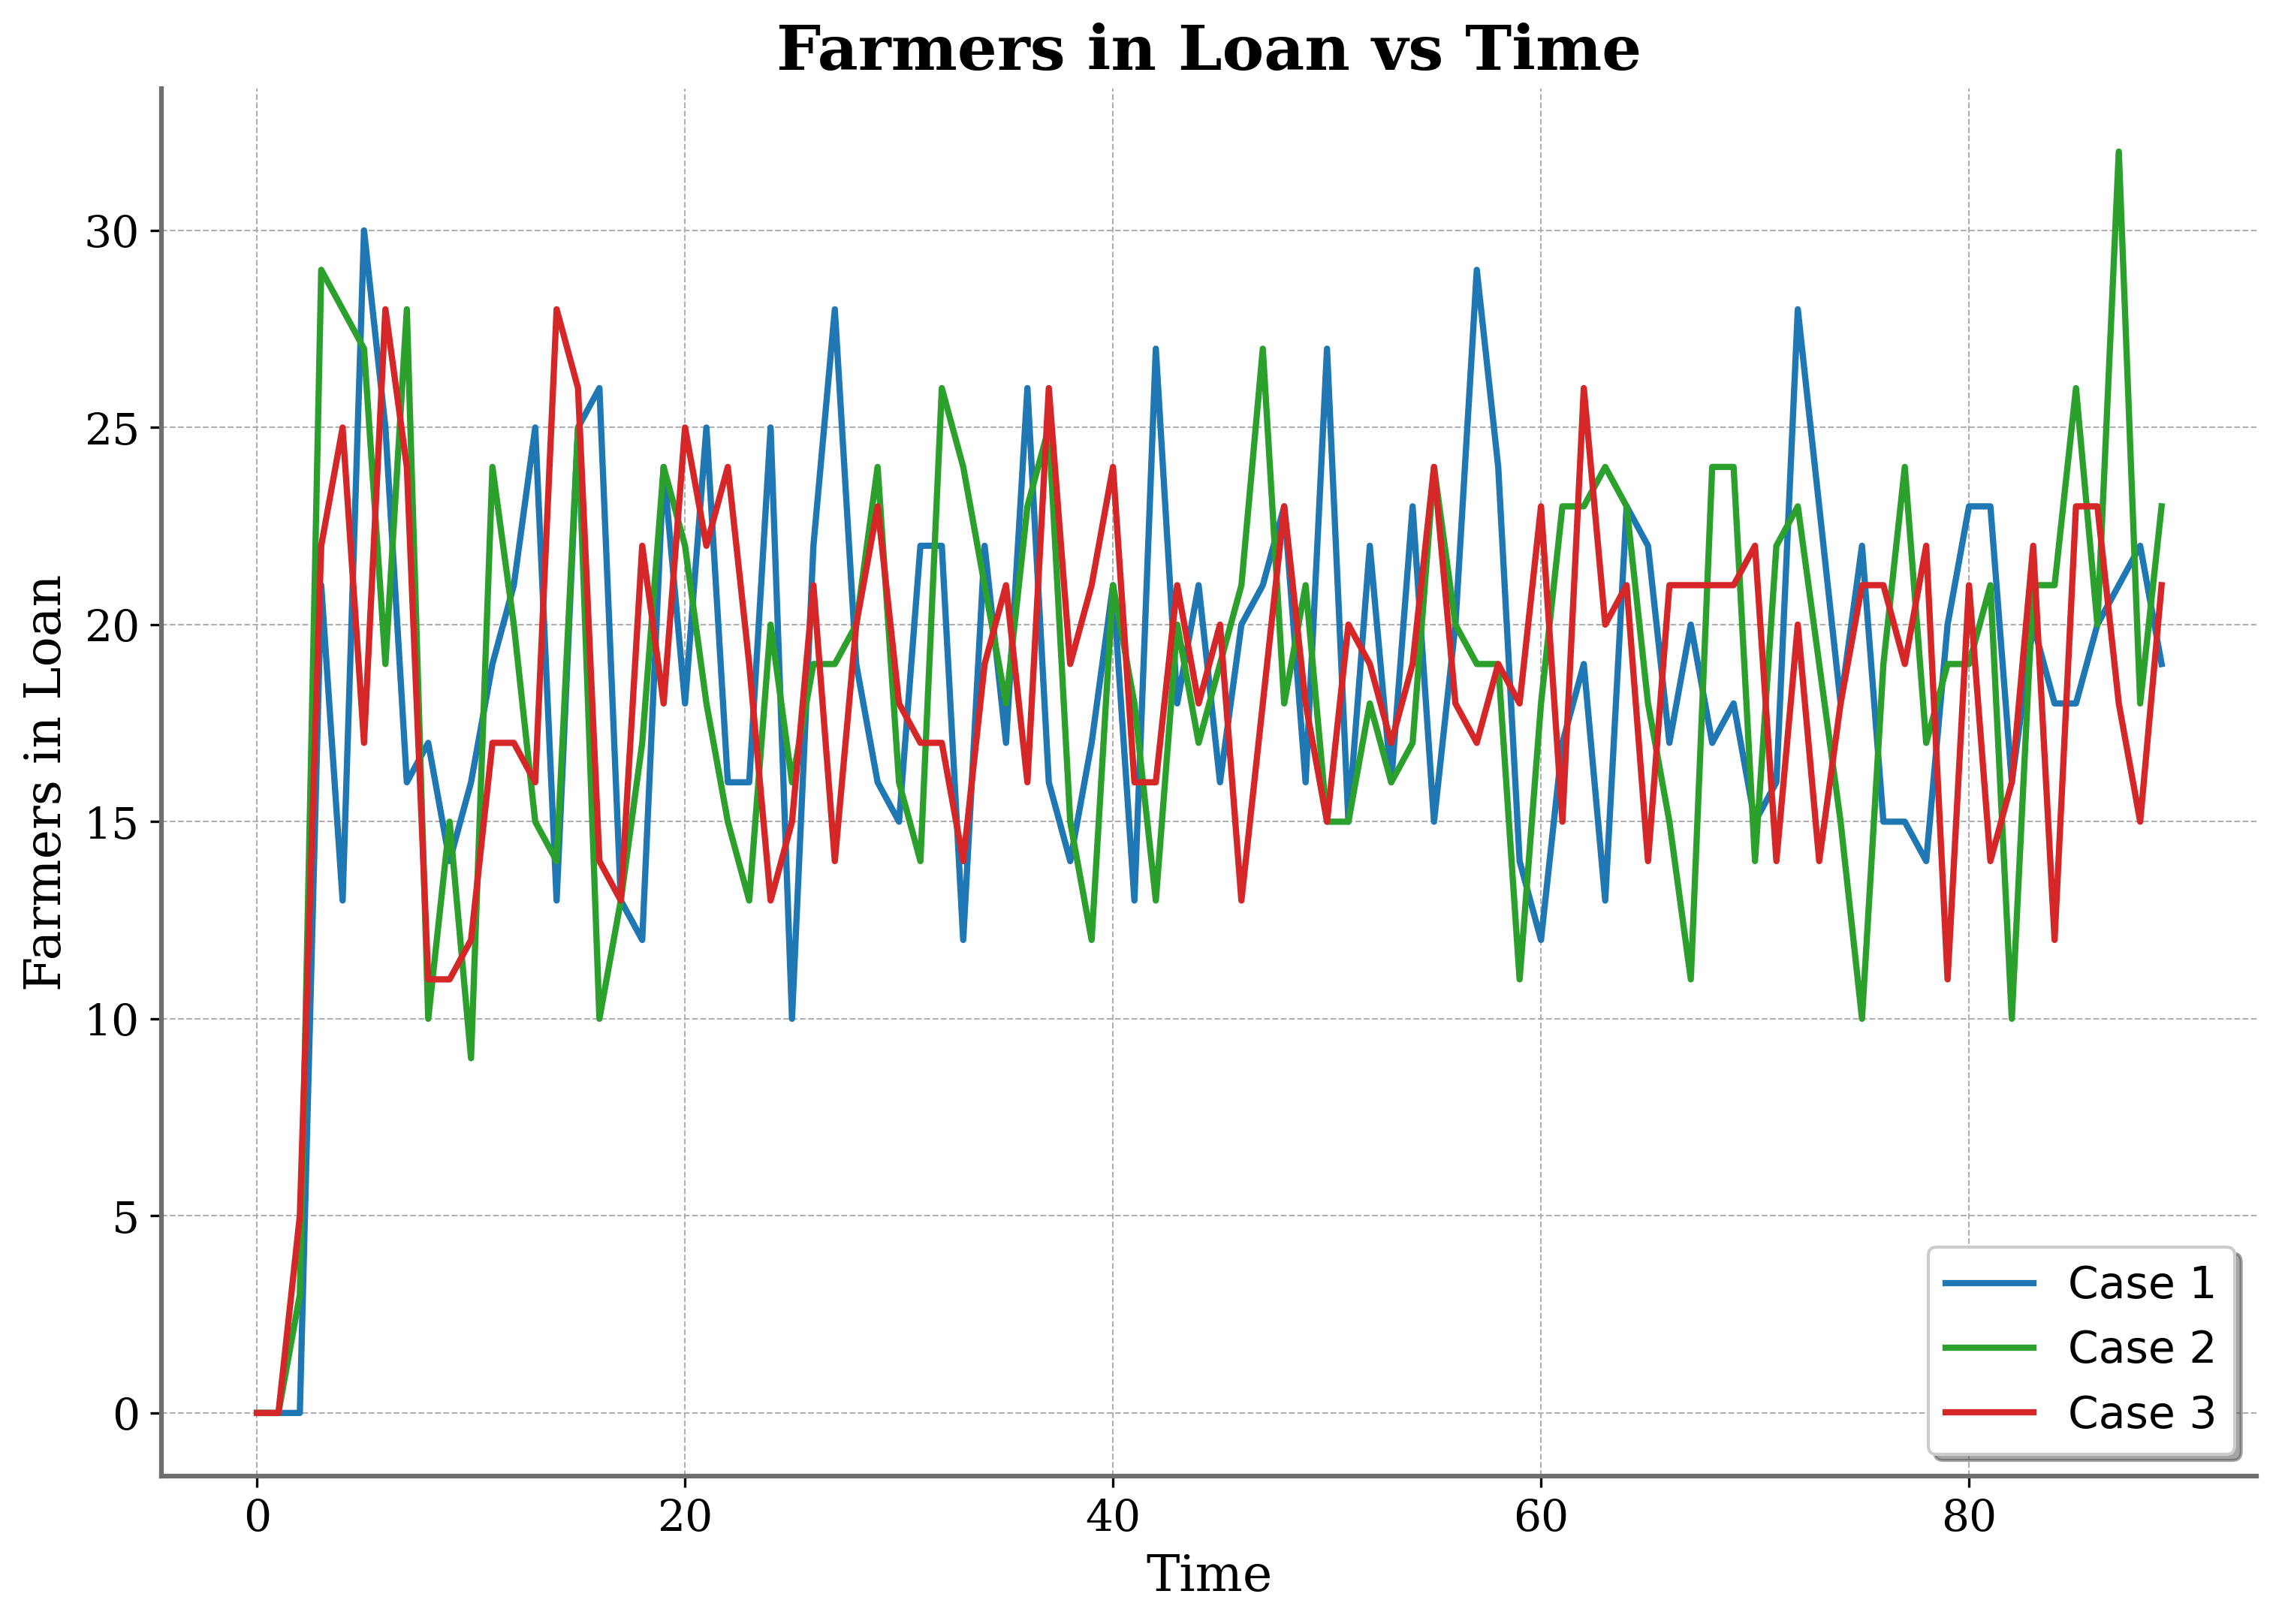
\includegraphics[width=0.4\textwidth]{graph_all/plots_fav/farmers_in_loan_vs_time.png}
    \caption{Farmers in Loan vs Time}
    \label{fig:farmers_loan}
\end{figure}
% Farmers in Loan - Statistical Analysis
\begin{table}[htbp]
    \centering
    \resizebox{0.4\textwidth}{!}{ % Adjust the 0.9 to control the table size
    \begin{tabular}{lccc}
        \toprule
        \textbf{Statistic} & \textbf{Case 1} & \textbf{Case 2} & \textbf{Case 3} \\
        \midrule
        Mean & 18.5889 & 18.6111 & 18.3667 \\
        Median & 18.5 & 19 & 19 \\
        Min & 0 & 0 & 0 \\
        Max & 30 & 32 & 28 \\
        Range & 30 & 32 & 28 \\
        Standard Deviation & 5.6467 & 5.83422 & 5.05353 \\
        Variance & 31.8853 & 34.0381 & 25.5382 \\
        Interquartile Range & 6 & 8 & 5 \\
        Skewness & -0.85729 & -0.72779 & -1.07787 \\
        Kurtosis & 2.04775 & 1.24838 & 2.51705 \\
        First Quartile & 16 & 15 & 16 \\
        Third Quartile & 22 & 23 & 21 \\
        MAD & 3.5 & 4 & 3 \\
        Coefficient of Variation & 0.30377 & 0.31348 & 0.27515 \\
        Mode & 16 & 19 & 21 \\
        \bottomrule
    \end{tabular}
    }
    \caption{Farmers in Loan - Statistical Analysis}
\end{table}
The loan measure for farmers (Figure 7 and Table 7) exhibits substantial temporal fluctuation, with three instances displaying significant overlap. The graph illustrates that farmers frequently necessitate loans at different points without displaying a discernible upward or downward pattern, implying an unstable or cyclical demand for financial assistance. The average values are similar, but the standard deviation and variation are greater compared to other analyses. The skewness and kurtosis data suggest that farmers use a wide range of loans. The analysis highlights the significance of flexible financial structures that can promptly react to changing lending requirements within the agricultural sector.\\
% Force all previous floats to be placed before continuing
\FloatBarrier

\subsubsection{Moderate Condition:}
\vspace{0.5cm}
The figures (8-16) and tables (8-16) illustrate the variations in results linked to the livelihood agents over time in the specified moderately challenging environment, comparable to the analysis conducted for the favourable condition. The X-axis indicates a single year, and each graph displays data for up to 90 years.

In this situation, the importance of the "Golpata Stock" remains crucial for the Bawali community, as it reflects the availability of resources under mild conditions. Similarly, the narratives named "Mangrove Fishers in Loan" and "Catching Capacity Mangrove" remain essential for mangrove fishers as they depict their reactions to unfavourable conditions. Similarly, the plots "Household Fishers in Loan" and "Catching Capacity Household" remain significant for household fisherman, as they depict the fluctuating patterns of loans and resources. Furthermore, the plots "Farmers in Loan" and "Crop Production Capacity" continue to be crucial for farmers, demonstrating their ability to adjust under modest circumstances.

The statistical indicators, such as those used to assess favourable conditions, enable a straightforward comparison among the three examples. The inclusion of these measures, in conjunction with the graphs, ensures a clear and unequivocal comprehension of the differences observed under different settings.\\
% First figure for Bawali
\begin{figure}[htbp]
    \centering
    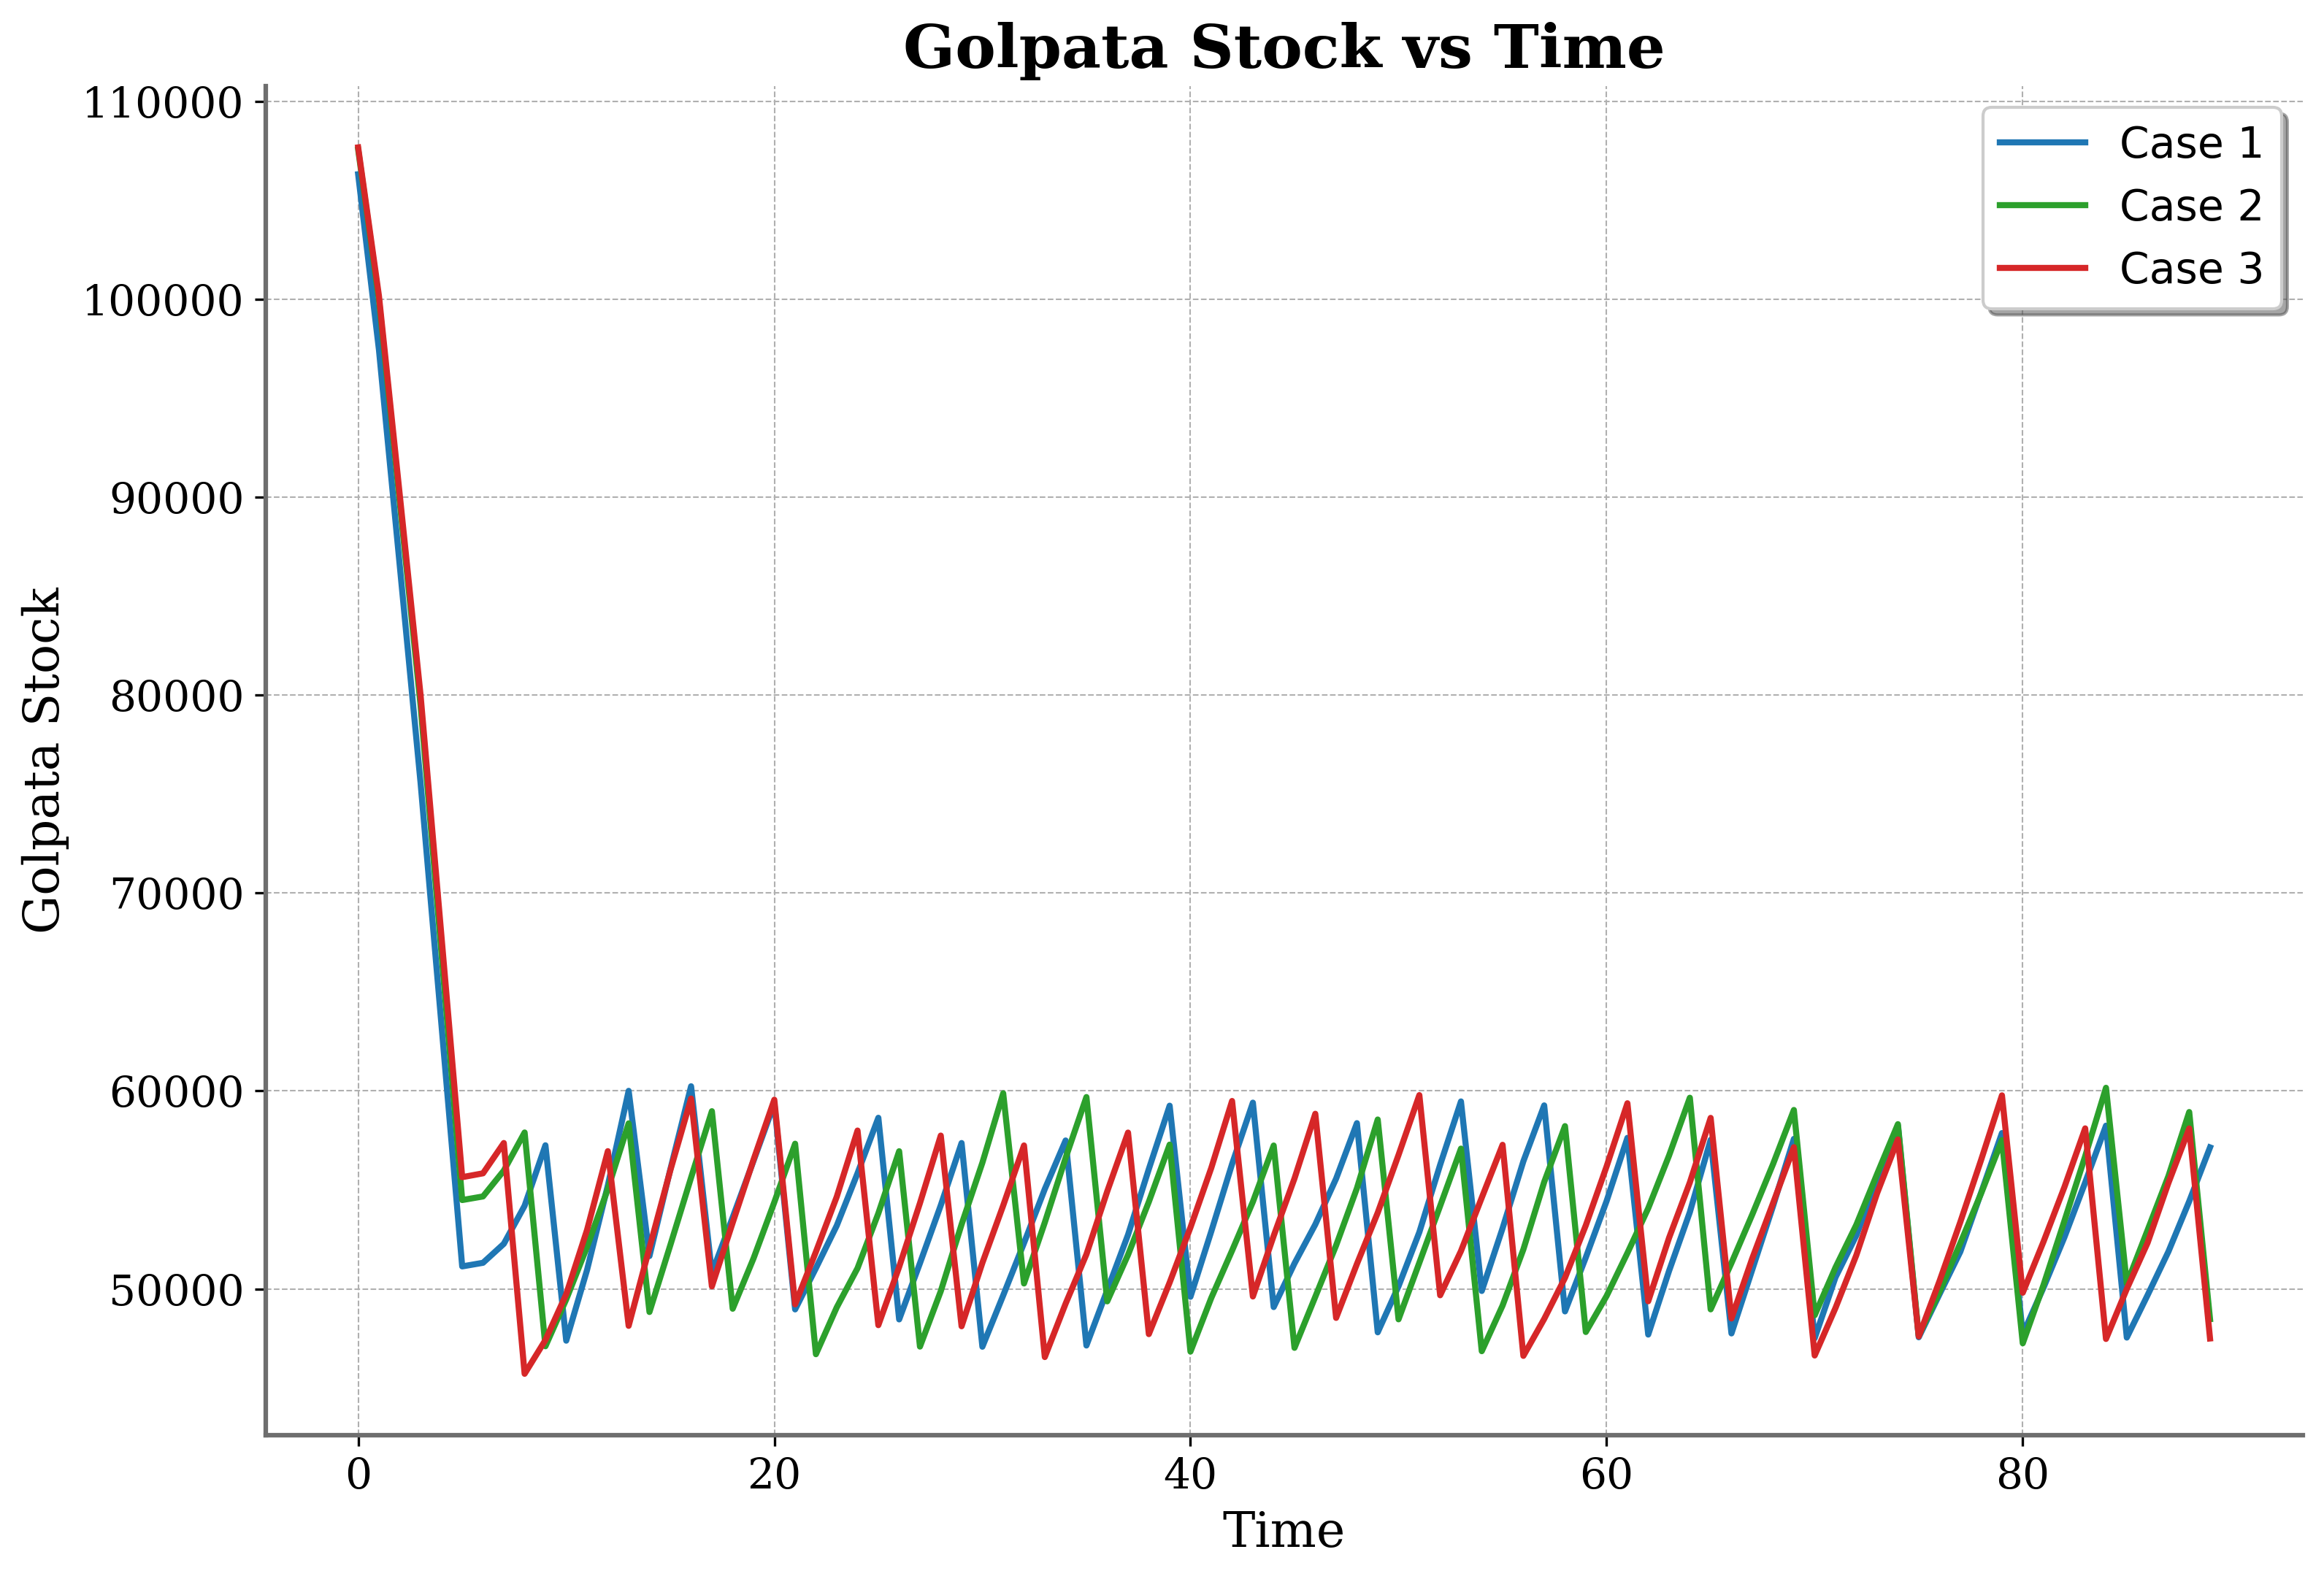
\includegraphics[width=0.4\textwidth]{graph_all/plots_mod/golpata_stock_vs_time.png}
    \caption{Golpata Stock vs Time for Bawali}
    \label{fig:bawali}
\end{figure}
% Golpata Stock - Statistical Analysis
\begin{table}[htbp]
    \centering
    \resizebox{0.4\textwidth}{!}{ % Adjust the 0.9 to control the table size
    \begin{tabular}{lccc}
        \toprule
        \textbf{Statistic} & \textbf{Case 1} & \textbf{Case 2} & \textbf{Case 3} \\
        \midrule
        Mean & 55087.02292 & 55121.24394 & 55129.37184 \\
        Median & 53222 & 53591.6 & 53360.8 \\
        Min & 47074.8 & 46696.8 & 45707.4 \\
        Max & 106312 & 107562 & 107669 \\
        Range & 59236.8 & 60864.8 & 61961.4 \\
        Standard Deviation & 9091.90399 & 9637.63072 & 9731.26996 \\
        Variance & 8.3e+07 & 9.3e+07 & 9.5e+07 \\
        Interquartile Range & 6589.99 & 7034.11 & 7254.51 \\
        Skewness & 3.66915 & 3.58458 & 3.53142 \\
        Kurtosis & 15.8102 & 14.7386 & 14.3647 \\
        First Quartile & 50635.6 & 49862.9 & 49851.4 \\
        Third Quartile & 57225.6 & 56897 & 57105.9 \\
        MAD & 3233.91 & 3571.18 & 3613.62 \\
        Coefficient of Variation & 0.16505 & 0.17484 & 0.17652 \\
        Mode & 47074.8 & 46696.8 & 45707.4 \\
        \bottomrule
    \end{tabular}
    }
    \caption{Golpata Stock - Statistical Analysis}
\end{table}
The Golpata Stock (Figure 8 and Table 8) , a resource stock in Bawali, has an initial sharp decline, but thereafter stabilises at a consistent level. Nevertheless, it consistently demonstrates variations during the remaining duration. The stock levels show slight variations, with Case 3 having the highest average stock level. Cases 2 and 3 demonstrate greater variability, suggesting increased volatility due to less stable extraction techniques or changeable environmental circumstances. The skewness and kurtosis measures suggest that the distribution exhibits a positive skewness, indicating a longer right tail, and a higher kurtosis, indicating a more peaked shape. The interquartile range (IQR) and variation are consistent with the overall patterns. Case 1 demonstrates a superior level of stability, whereas Cases 2 and 3 display a higher degree of variability. These findings emphasise the need for tailored strategies to minimise variations in the Golpata stock during less severe conditions.\\
% Second figure for Mangrove Fishermen
\begin{figure}[htbp]
    \centering
    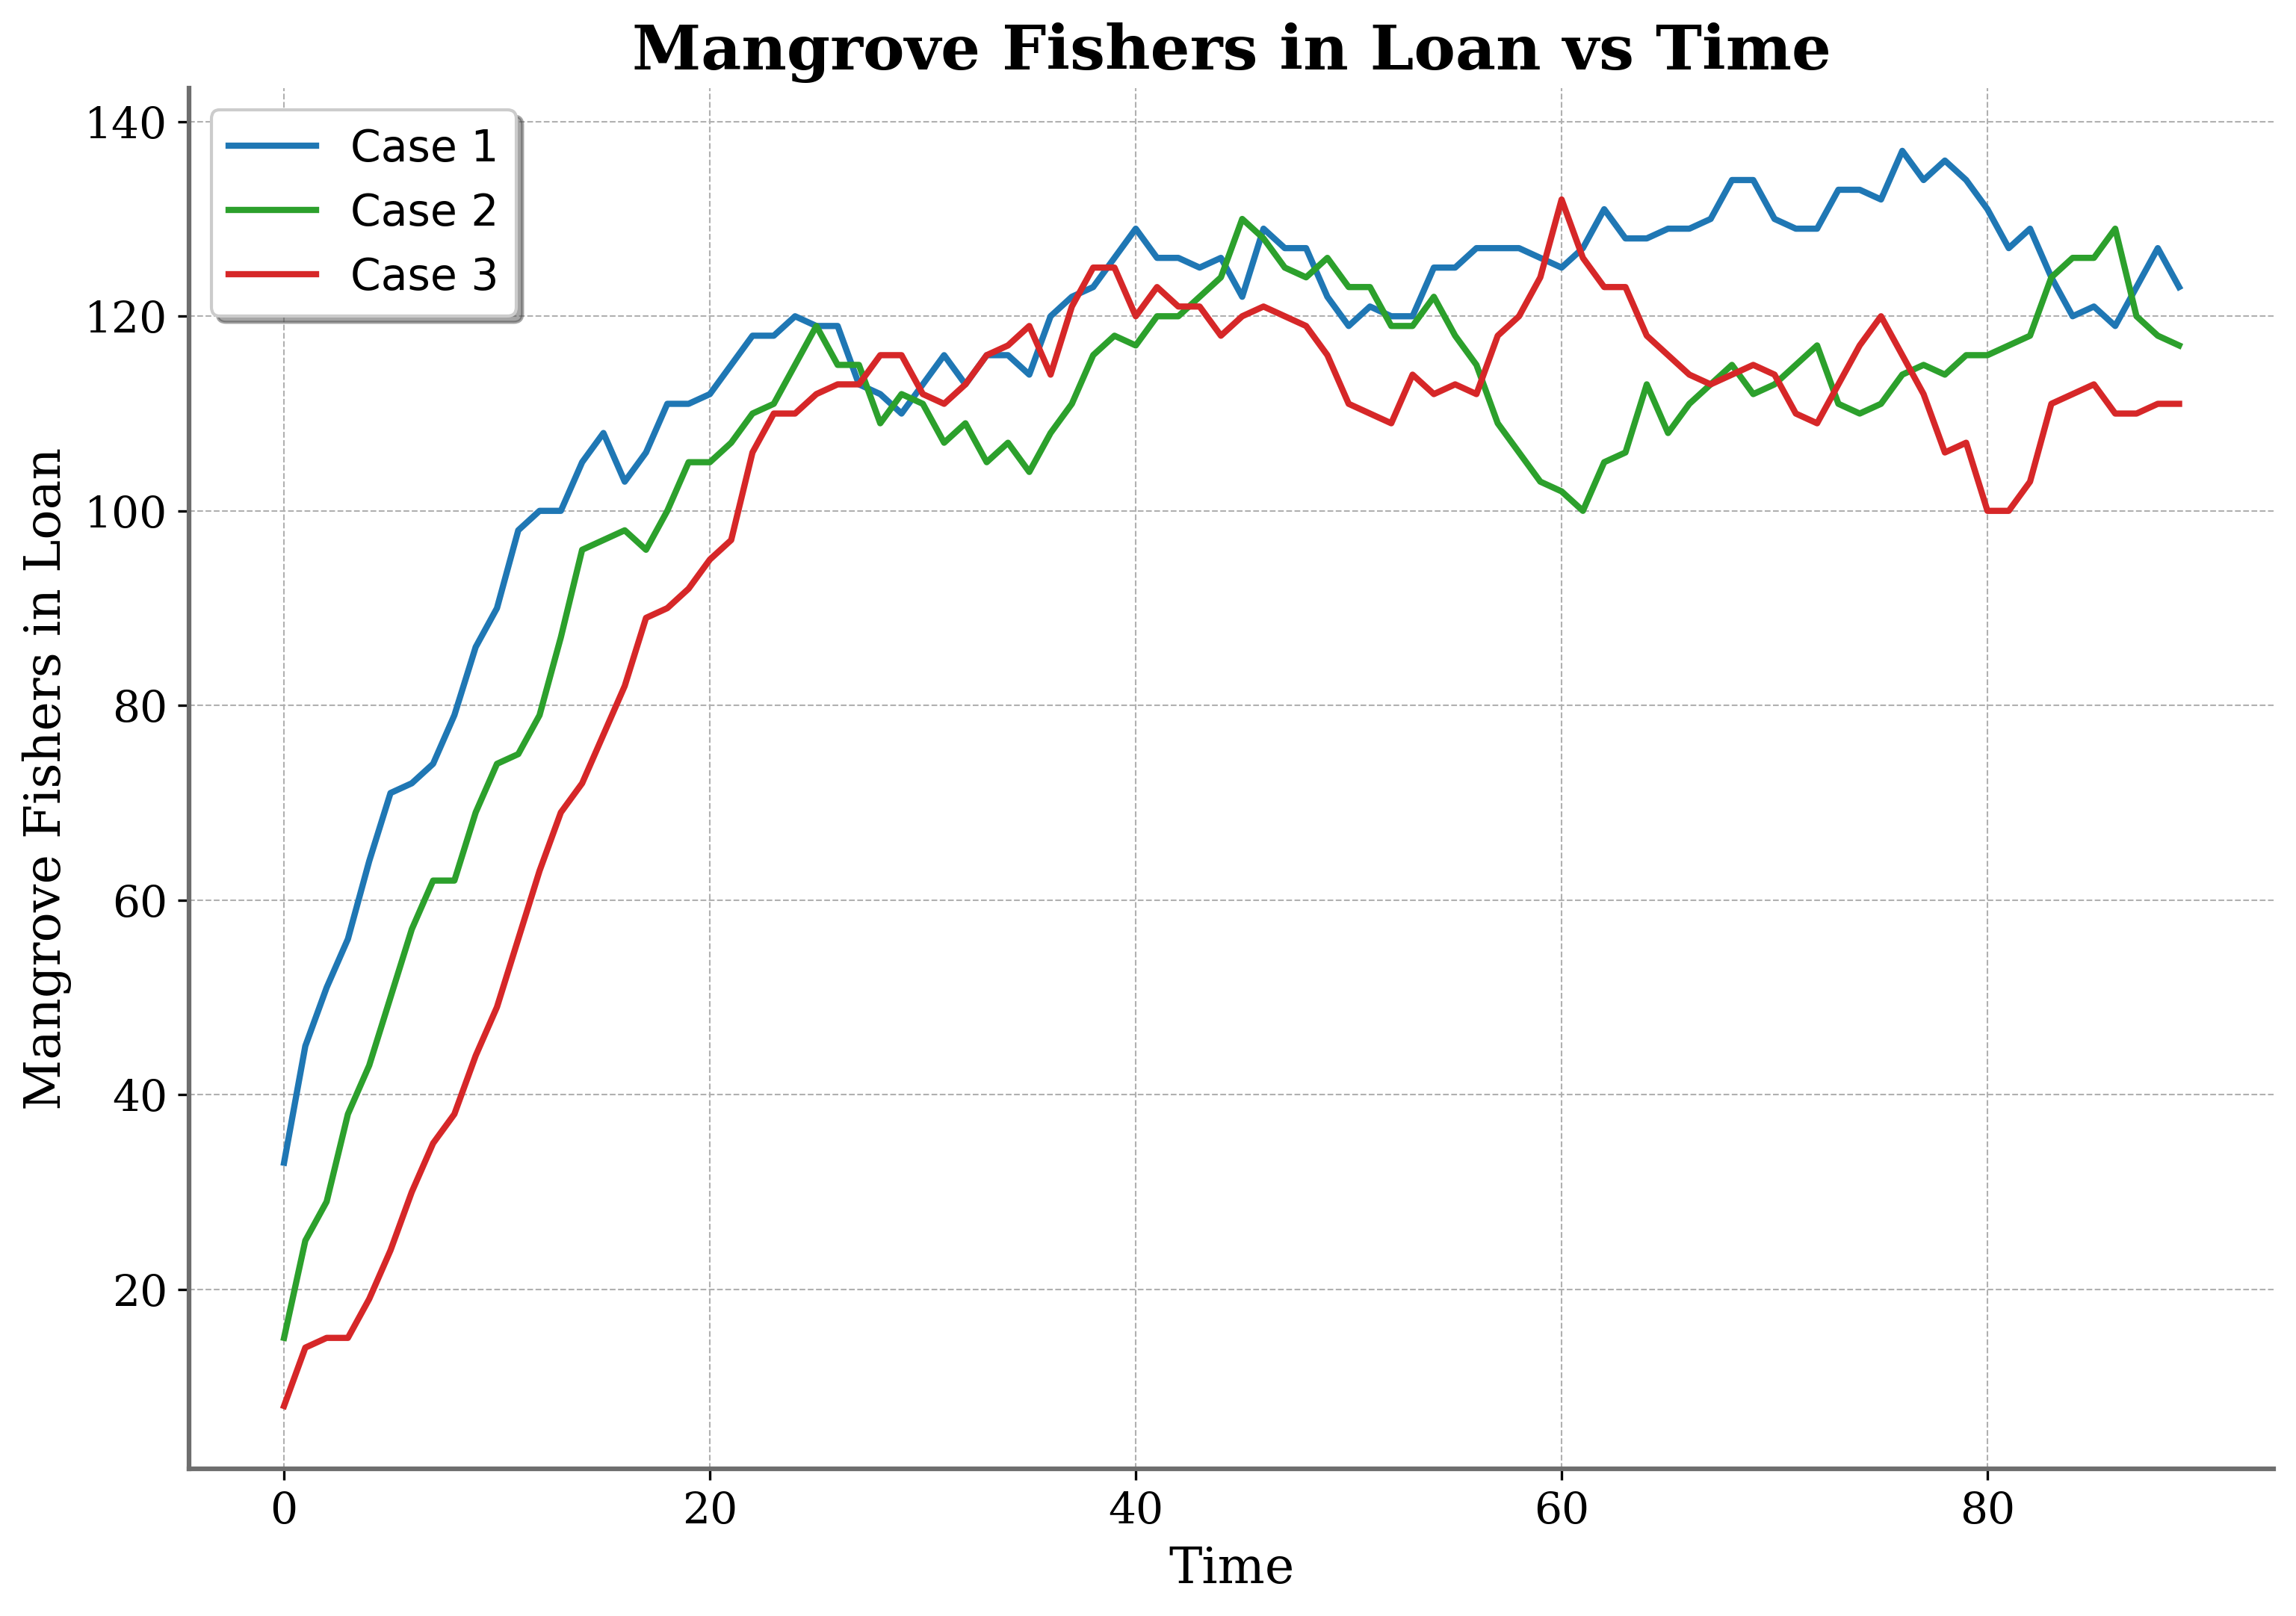
\includegraphics[width=0.4\textwidth]{graph_all/plots_mod/mangrove_fishers_in_loan_vs_time.png}
    \caption{Mangrove Fishers in Loan vs Time}
    \label{fig:mangrove_loan}
\end{figure}
\begin{table}[htbp]
    \centering
    \resizebox{0.4\textwidth}{!}{ % Adjust the 0.9 to control the table size
    \begin{tabular}{lccc}
        \toprule
        \textbf{Statistic} & \textbf{Case 1} & \textbf{Case 2} & \textbf{Case 3} \\
        \midrule
        Mean & 115.1111111 & 104.4 & 99.81111111 \\
        Median & 122 & 111.5 & 112 \\
        Min & 33 & 15 & 8 \\
        Max & 137 & 130 & 132 \\
        Range & 104 & 115 & 124 \\
        Standard Deviation & 21.2176757 & 24.2268307 & 30.9050356 \\
        Variance & 450.19 & 586.939 & 955.121 \\
        Interquartile Range & 14.75 & 13.75 & 17 \\
        Skewness & -2.02553 & -2.00273 & -1.76297 \\
        Kurtosis & 3.76952 & 3.50148 & 1.87433 \\
        First Quartile & 112.25 & 104.25 & 100 \\
        Third Quartile & 127 & 118 & 117 \\
        MAD & 7 & 6.5 & 6 \\
        Coefficient of Variation & 0.18432 & 0.23206 & 0.30964 \\
        Mode & 127 & 115 & 113 \\
        \bottomrule
    \end{tabular}
    }
    \caption{Mangrove Fishers in Loan - Statistical Analysis}
\end{table}
The analysis of Mangrove Fishers (Figure 9 and Table 9) in Loan shows a stable environment in Case 1, with a steady increase in loan participation. However, Cases 2 and 3 show greater variability, with smaller average numbers and wider ranges, indicating increased unpredictability. The analysis also shows negative skewness and high kurtosis values, suggesting that most fisher behavior is concentrated within specific lower ranges. The moderate situation offers greater resilience in Case 1, but specific actions may be needed to reduce risks and ensure seamless involvement in loans for mangrove fishers in changing circumstances.\\
% Third figure for Catching Capacity Mangrove
\begin{figure}[htbp]
    \centering
    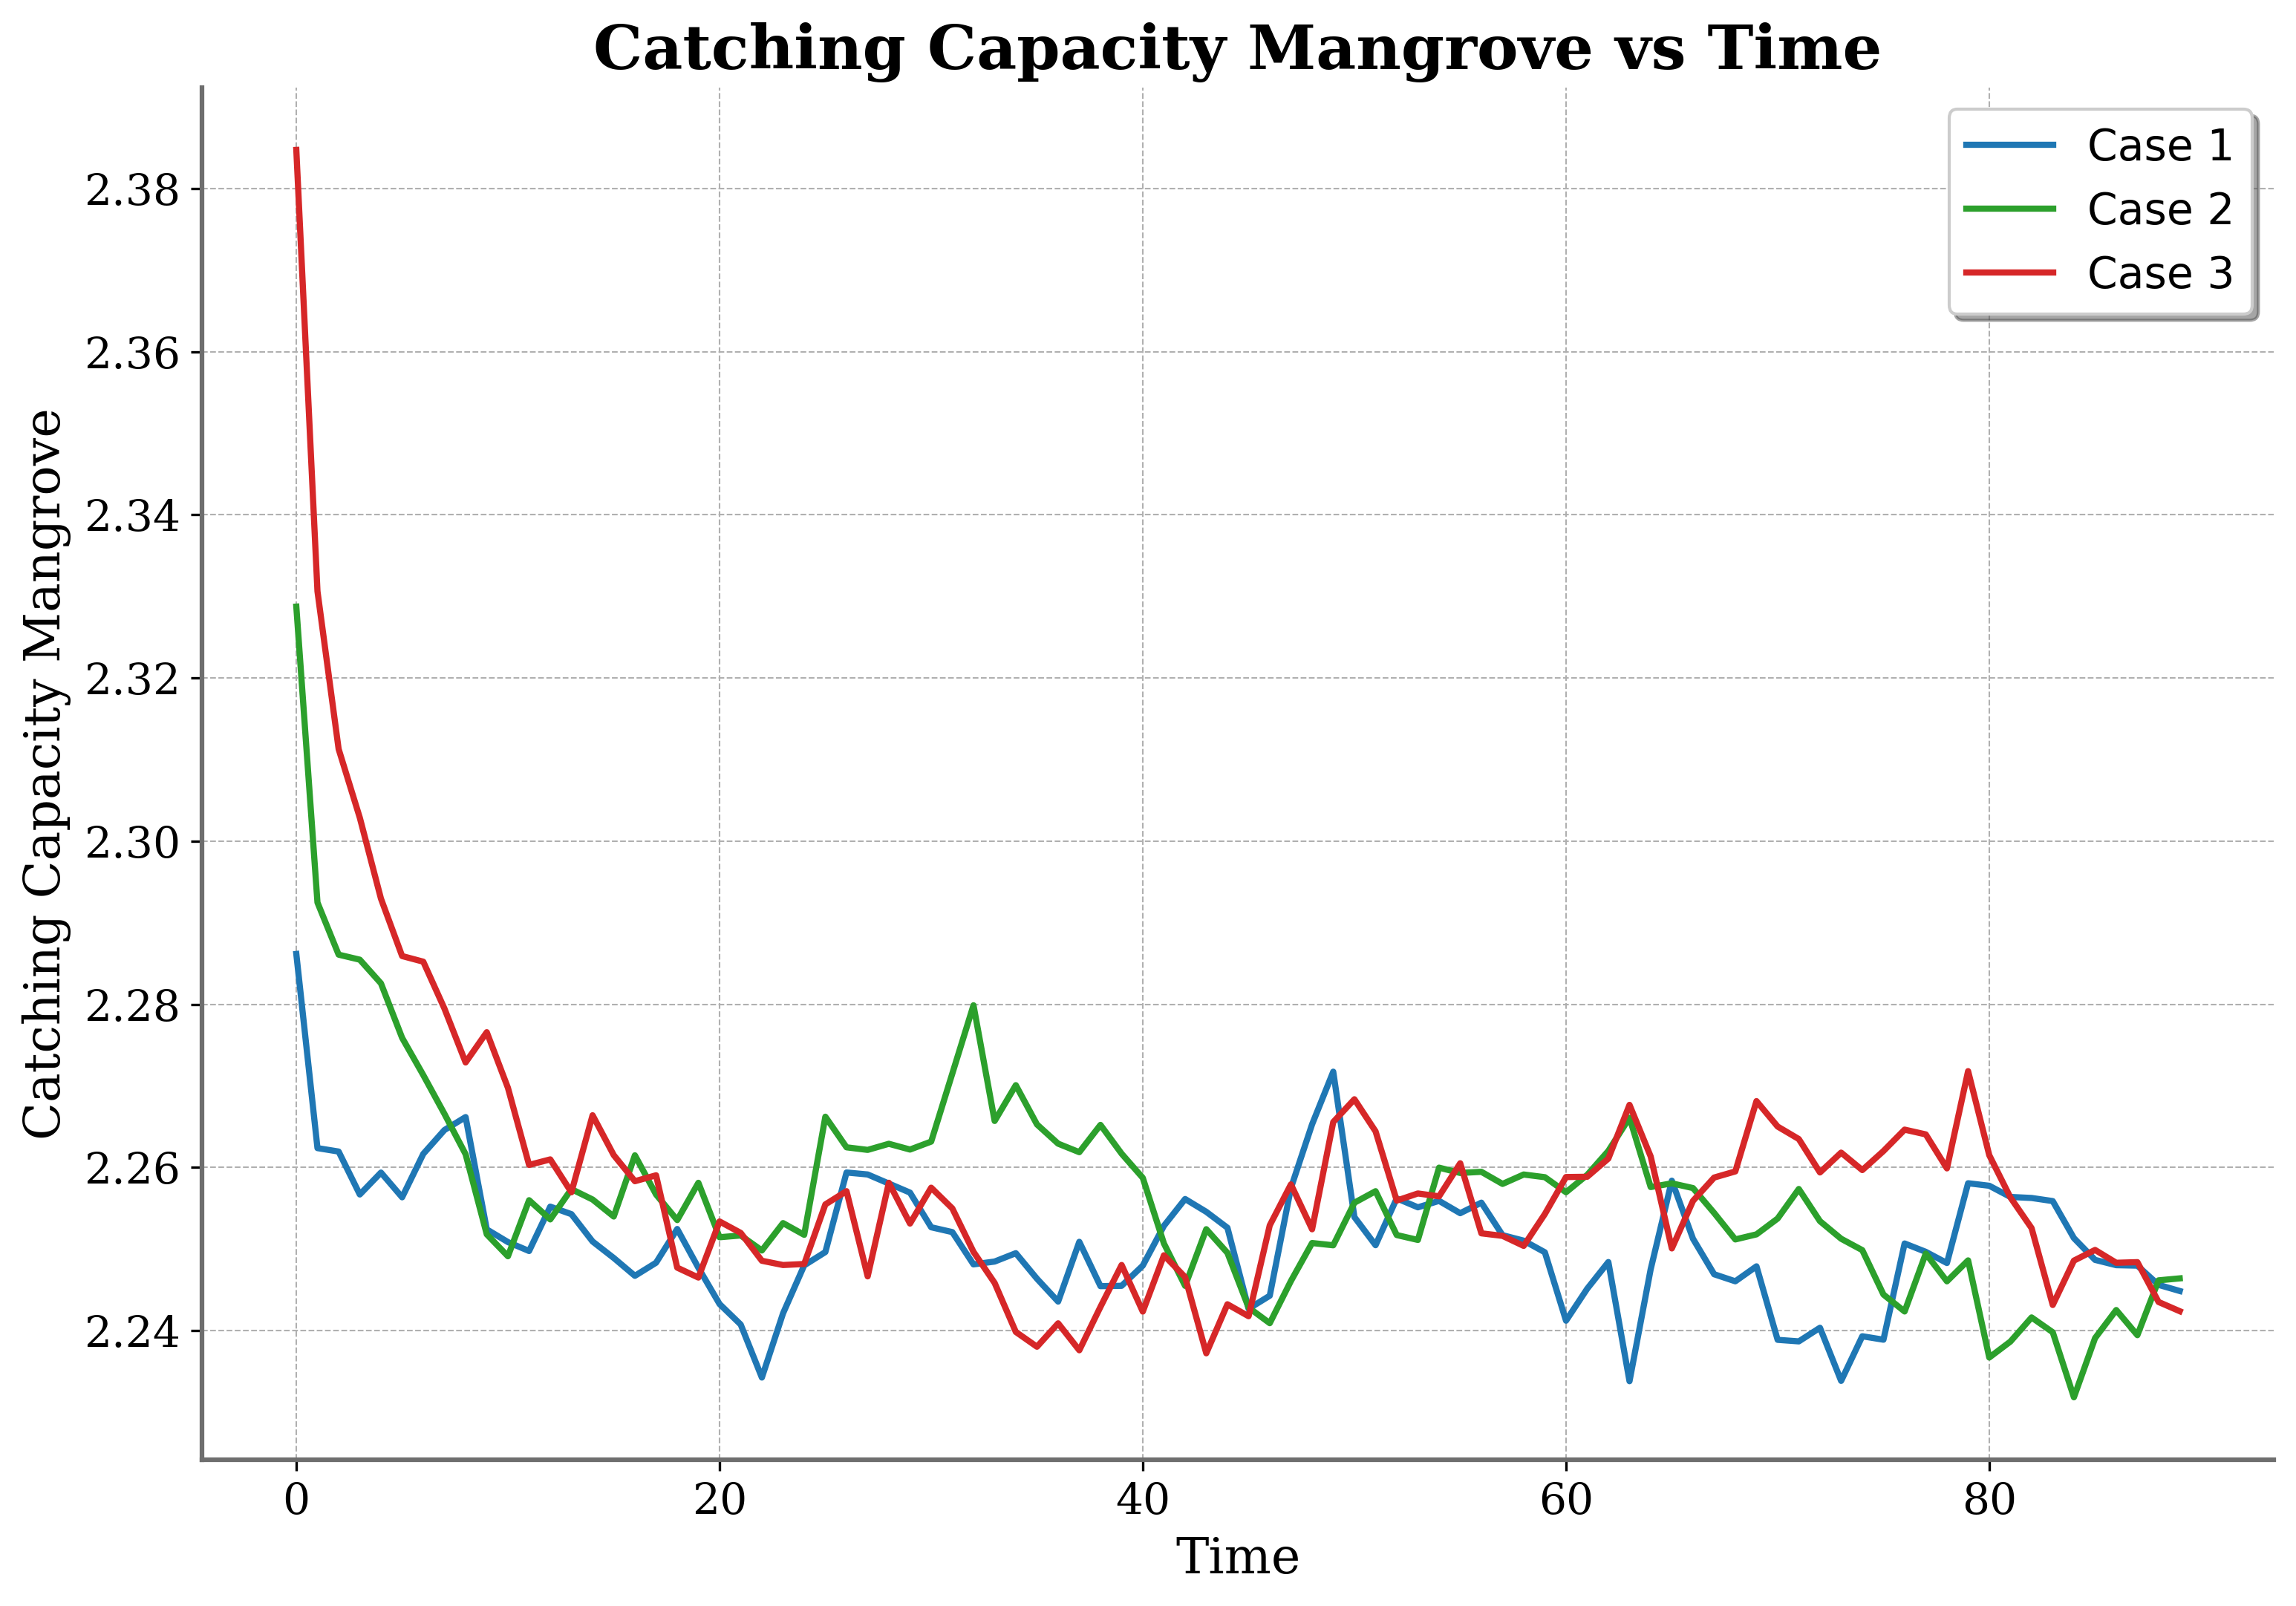
\includegraphics[width=0.4\textwidth]{graph_all/plots_mod/catching_capacity_mangrove_vs_time.png}
    \caption{Catching Capacity Mangrove vs Time}
    \label{fig:catching_mangrove}
\end{figure}
% Catching Capacity Mangrove - Statistical Analysis
\begin{table}[htbp]
    \centering
    \resizebox{0.4\textwidth}{!}{ % Adjust the 0.9 to control the table size
    \begin{tabular}{lccc}
        \toprule
        \textbf{Statistic} & \textbf{Case 1} & \textbf{Case 2} & \textbf{Case 3} \\
        \midrule
        Mean & 2.25112908 & 2.257005464 & 2.259683529 \\
        Median & 2.25076 & 2.25602 & 2.25688 \\
        Min & 2.23379 & 2.23182 & 2.23721 \\
        Max & 2.28617 & 2.32875 & 2.38474 \\
        Range & 0.05238 & 0.09693 & 0.14753 \\
        Standard Deviation & 0.00814895 & 0.01342146 & 0.02017058 \\
        Variance & 6.64e-05 & 0.00018 & 0.00041 \\
        Interquartile Range & 0.00931 & 0.01198 & 0.0134 \\
        Skewness & 0.81171 & 2.02505 & 3.45805 \\
        Kurtosis & 2.92764 & 8.13363 & 16.5492 \\
        First Quartile & 2.24675 & 2.25 & 2.24856 \\
        Third Quartile & 2.25607 & 2.26198 & 2.26196 \\
        MAD & 0.00501 & 0.00606 & 0.00739 \\
        Coefficient of Variation & 0.00362 & 0.00595 & 0.00893 \\
        Mode & 2.23379 & 2.23182 & 2.23721 \\
        \bottomrule
    \end{tabular}
    }
    \caption{Catching Capacity Mangrove - Statistical Analysis}
\end{table}
The study assesses the capacities for fishermen of mangroves (Figure 10 and Table 10) in three separate circumstances. Case 1 exhibits a stable catching capacity, characterised by an average value of 2.2511 and a low standard deviation. Case 2 has higher variability, characterised by a wider range and a bigger standard deviation. Case 3 has the greatest degree of volatility, characterised by the highest average value and the largest standard deviation. The study indicates that Case 1 provides a more consistent environment for retaining the potential of mangroves, but Cases 2 and 3 exhibit higher levels of variability. This underscores the necessity of implementing targeted management strategies to reduce fluctuations and enhance stability.\\
% Fourth figure for Household Fishers in Loan
\begin{figure}[htbp]
    \centering
    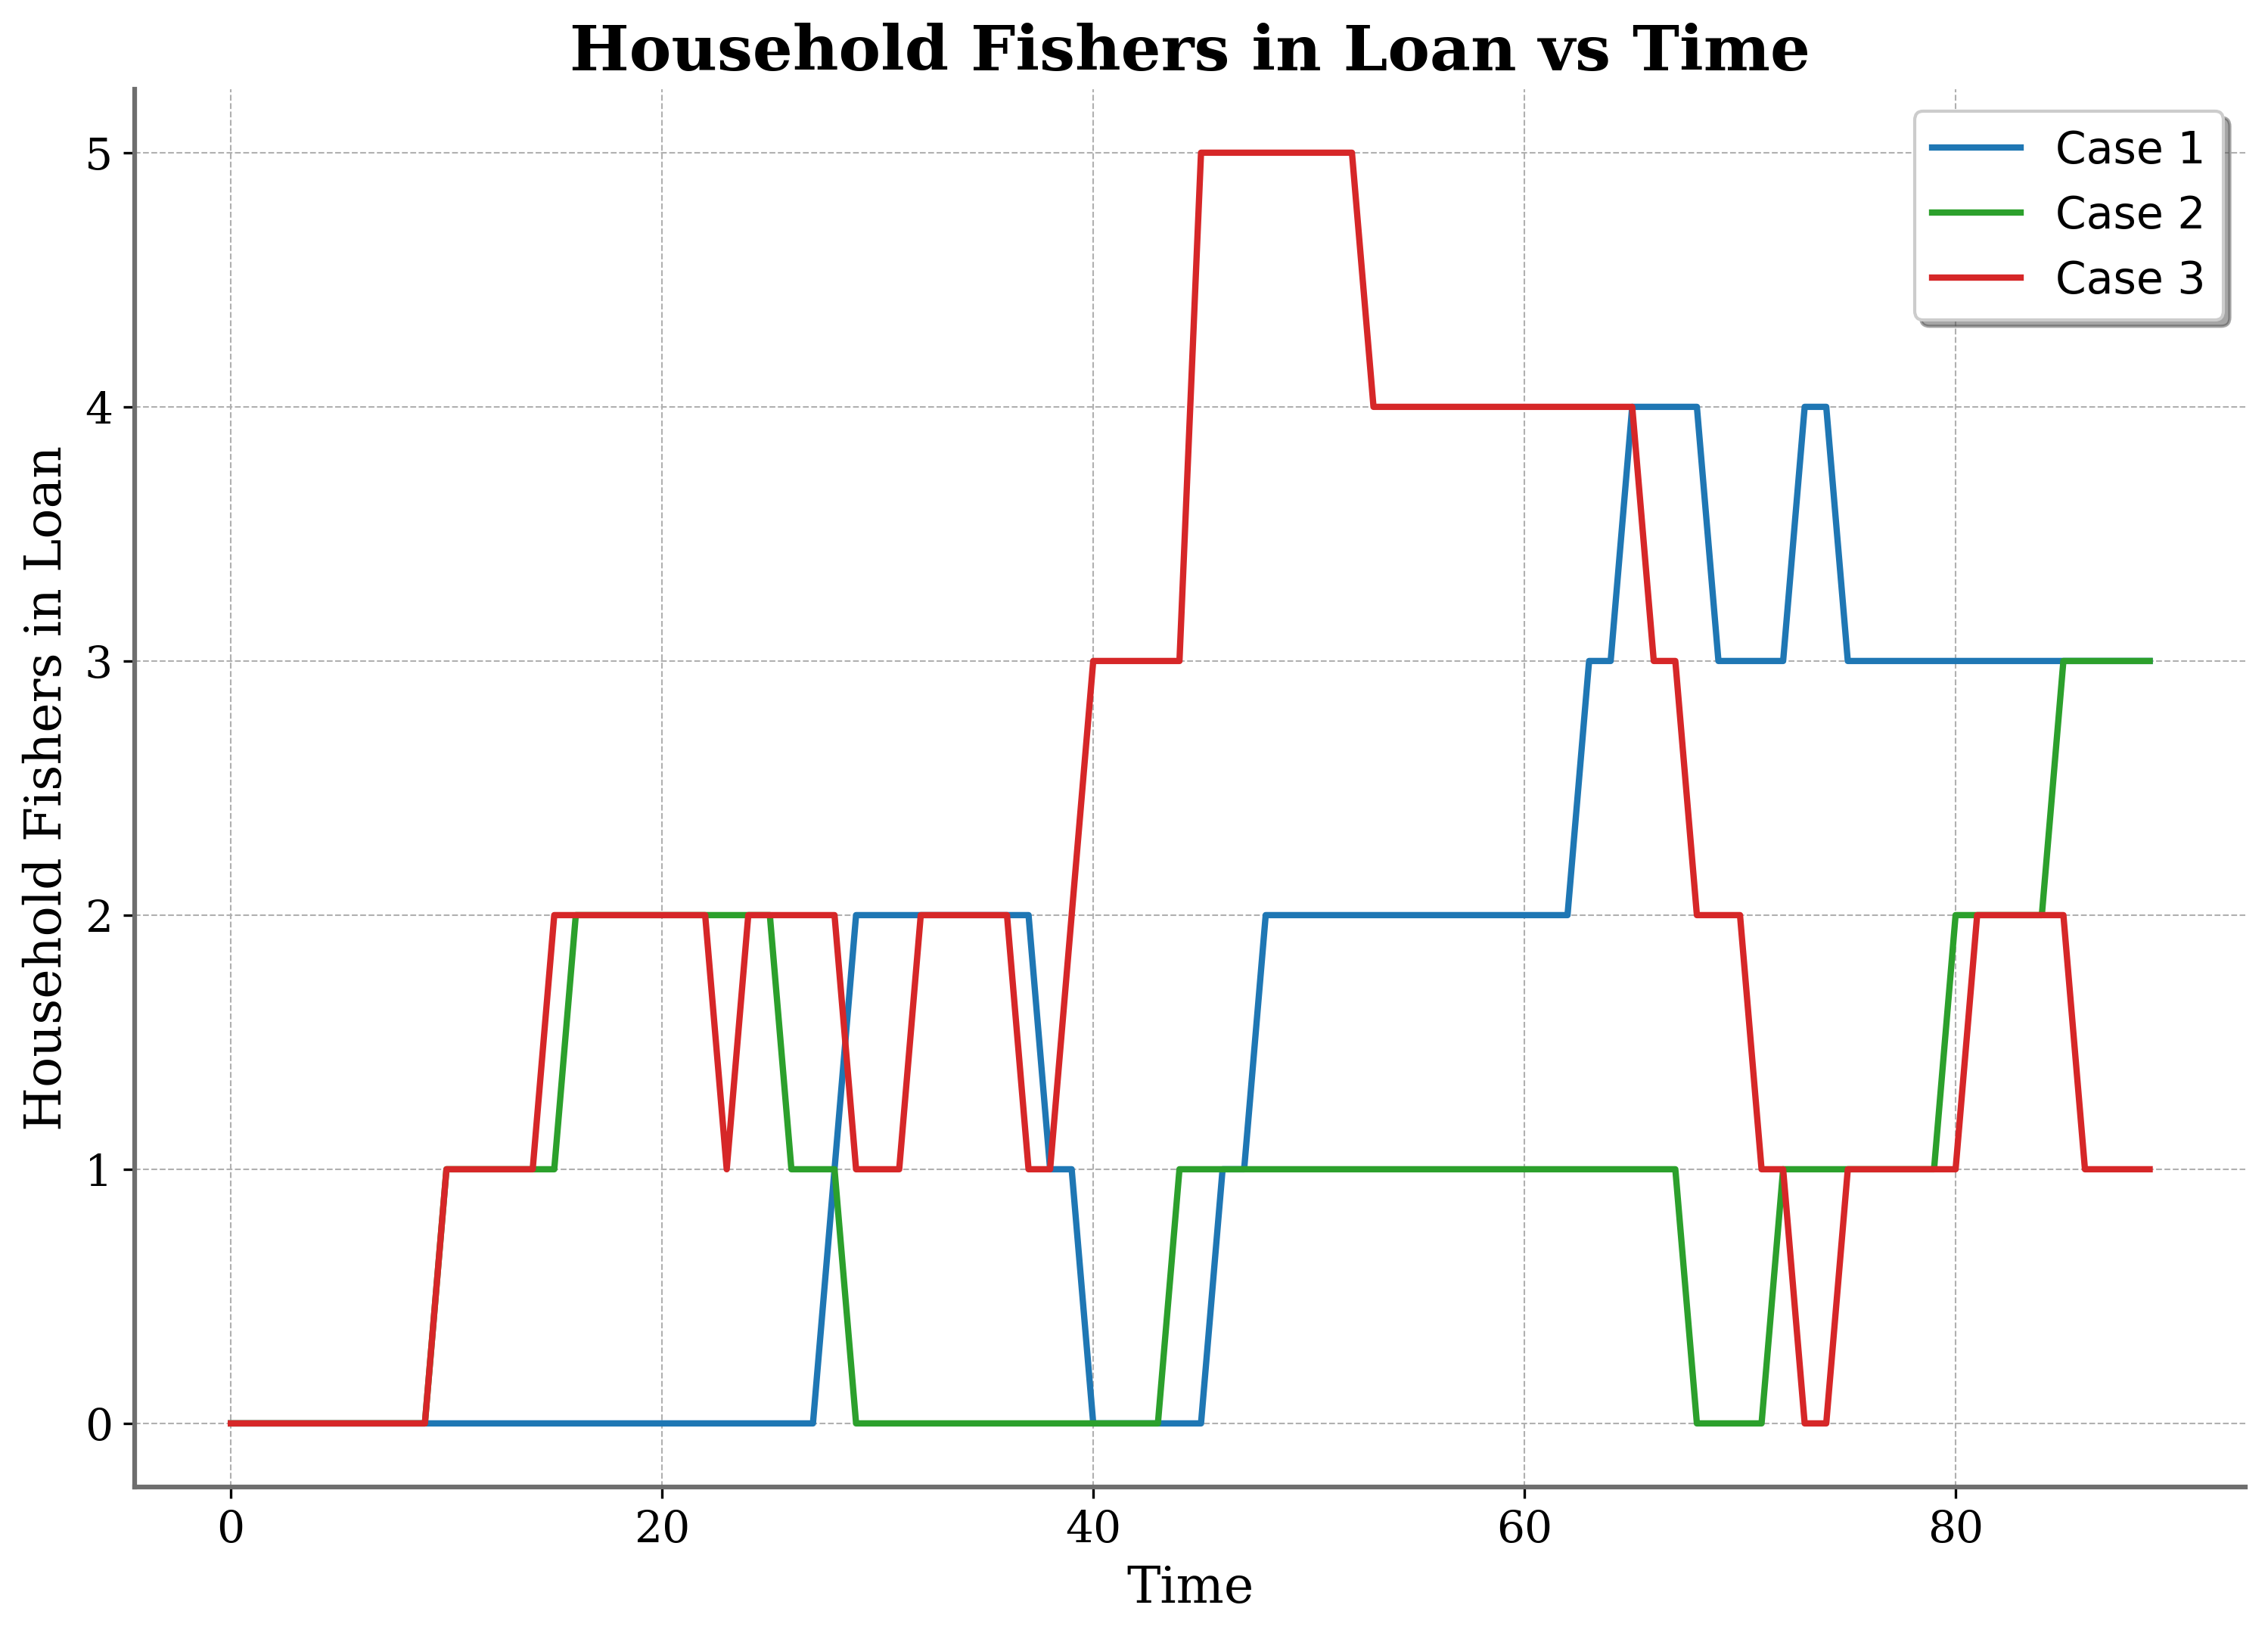
\includegraphics[width=0.4\textwidth]{graph_all/plots_mod/household_fishers_in_loan_vs_time.png}
    \caption{Household Fishers in Loan vs Time}
    \label{fig:household_loan}
\end{figure}
\begin{table}[htbp]
    \centering
    \resizebox{0.4\textwidth}{!}{ % Adjust the 0.9 to control the table size
    \begin{tabular}{lccc}
        \toprule
        \textbf{Statistic} & \textbf{Case 1} & \textbf{Case 2} & \textbf{Case 3} \\
        \midrule
        Mean & 1.555555556 & 0.955555556 & 2.111111111 \\
        Median & 2 & 1 & 2 \\
        Min & 0 & 0 & 0 \\
        Max & 4 & 3 & 5 \\
        Range & 4 & 3 & 5 \\
        Standard Deviation & 1.37482265 & 0.84681971 & 1.50239094 \\
        Variance & 1.89014 & 0.7171 & 2.25718 \\
        Interquartile Range & 3 & 1 & 2 \\
        Skewness & 0.10521 & 0.64225 & 0.46951 \\
        Kurtosis & -1.39032 & -0.14133 & -0.7688 \\
        First Quartile & 0 & 0 & 1 \\
        Third Quartile & 3 & 1 & 3 \\
        MAD & 1 & 1 & 1 \\
        Coefficient of Variation & 0.88381 & 0.88621 & 0.71166 \\
        Mode & 0 & 1 & 2 \\
        \bottomrule
    \end{tabular}
    }
    \caption{Household Fishers in Loan - Statistical Analysis}
\end{table}
The study examines loan conditions among household fishers (Figure 11 and Table 11)  in a minimally regulated setting. The results show fluctuating levels of participation across three examples, with significant disparities in consistency and magnitude. Case 1 has a moderate level of engagement, with an average of 1.56 participants. Case 2 has lower participation, with an average of 0.96 participants. Case 3 has the highest average value and greatest variability, with a higher occurrence of low loan participation with occasional spikes. The study highlights the importance of stabilizing economic conditions to ensure consistent financial conduct among family fishers in various situations.\\
% Fifth figure for Catching Capacity Household
\begin{figure}[htbp]
    \centering
    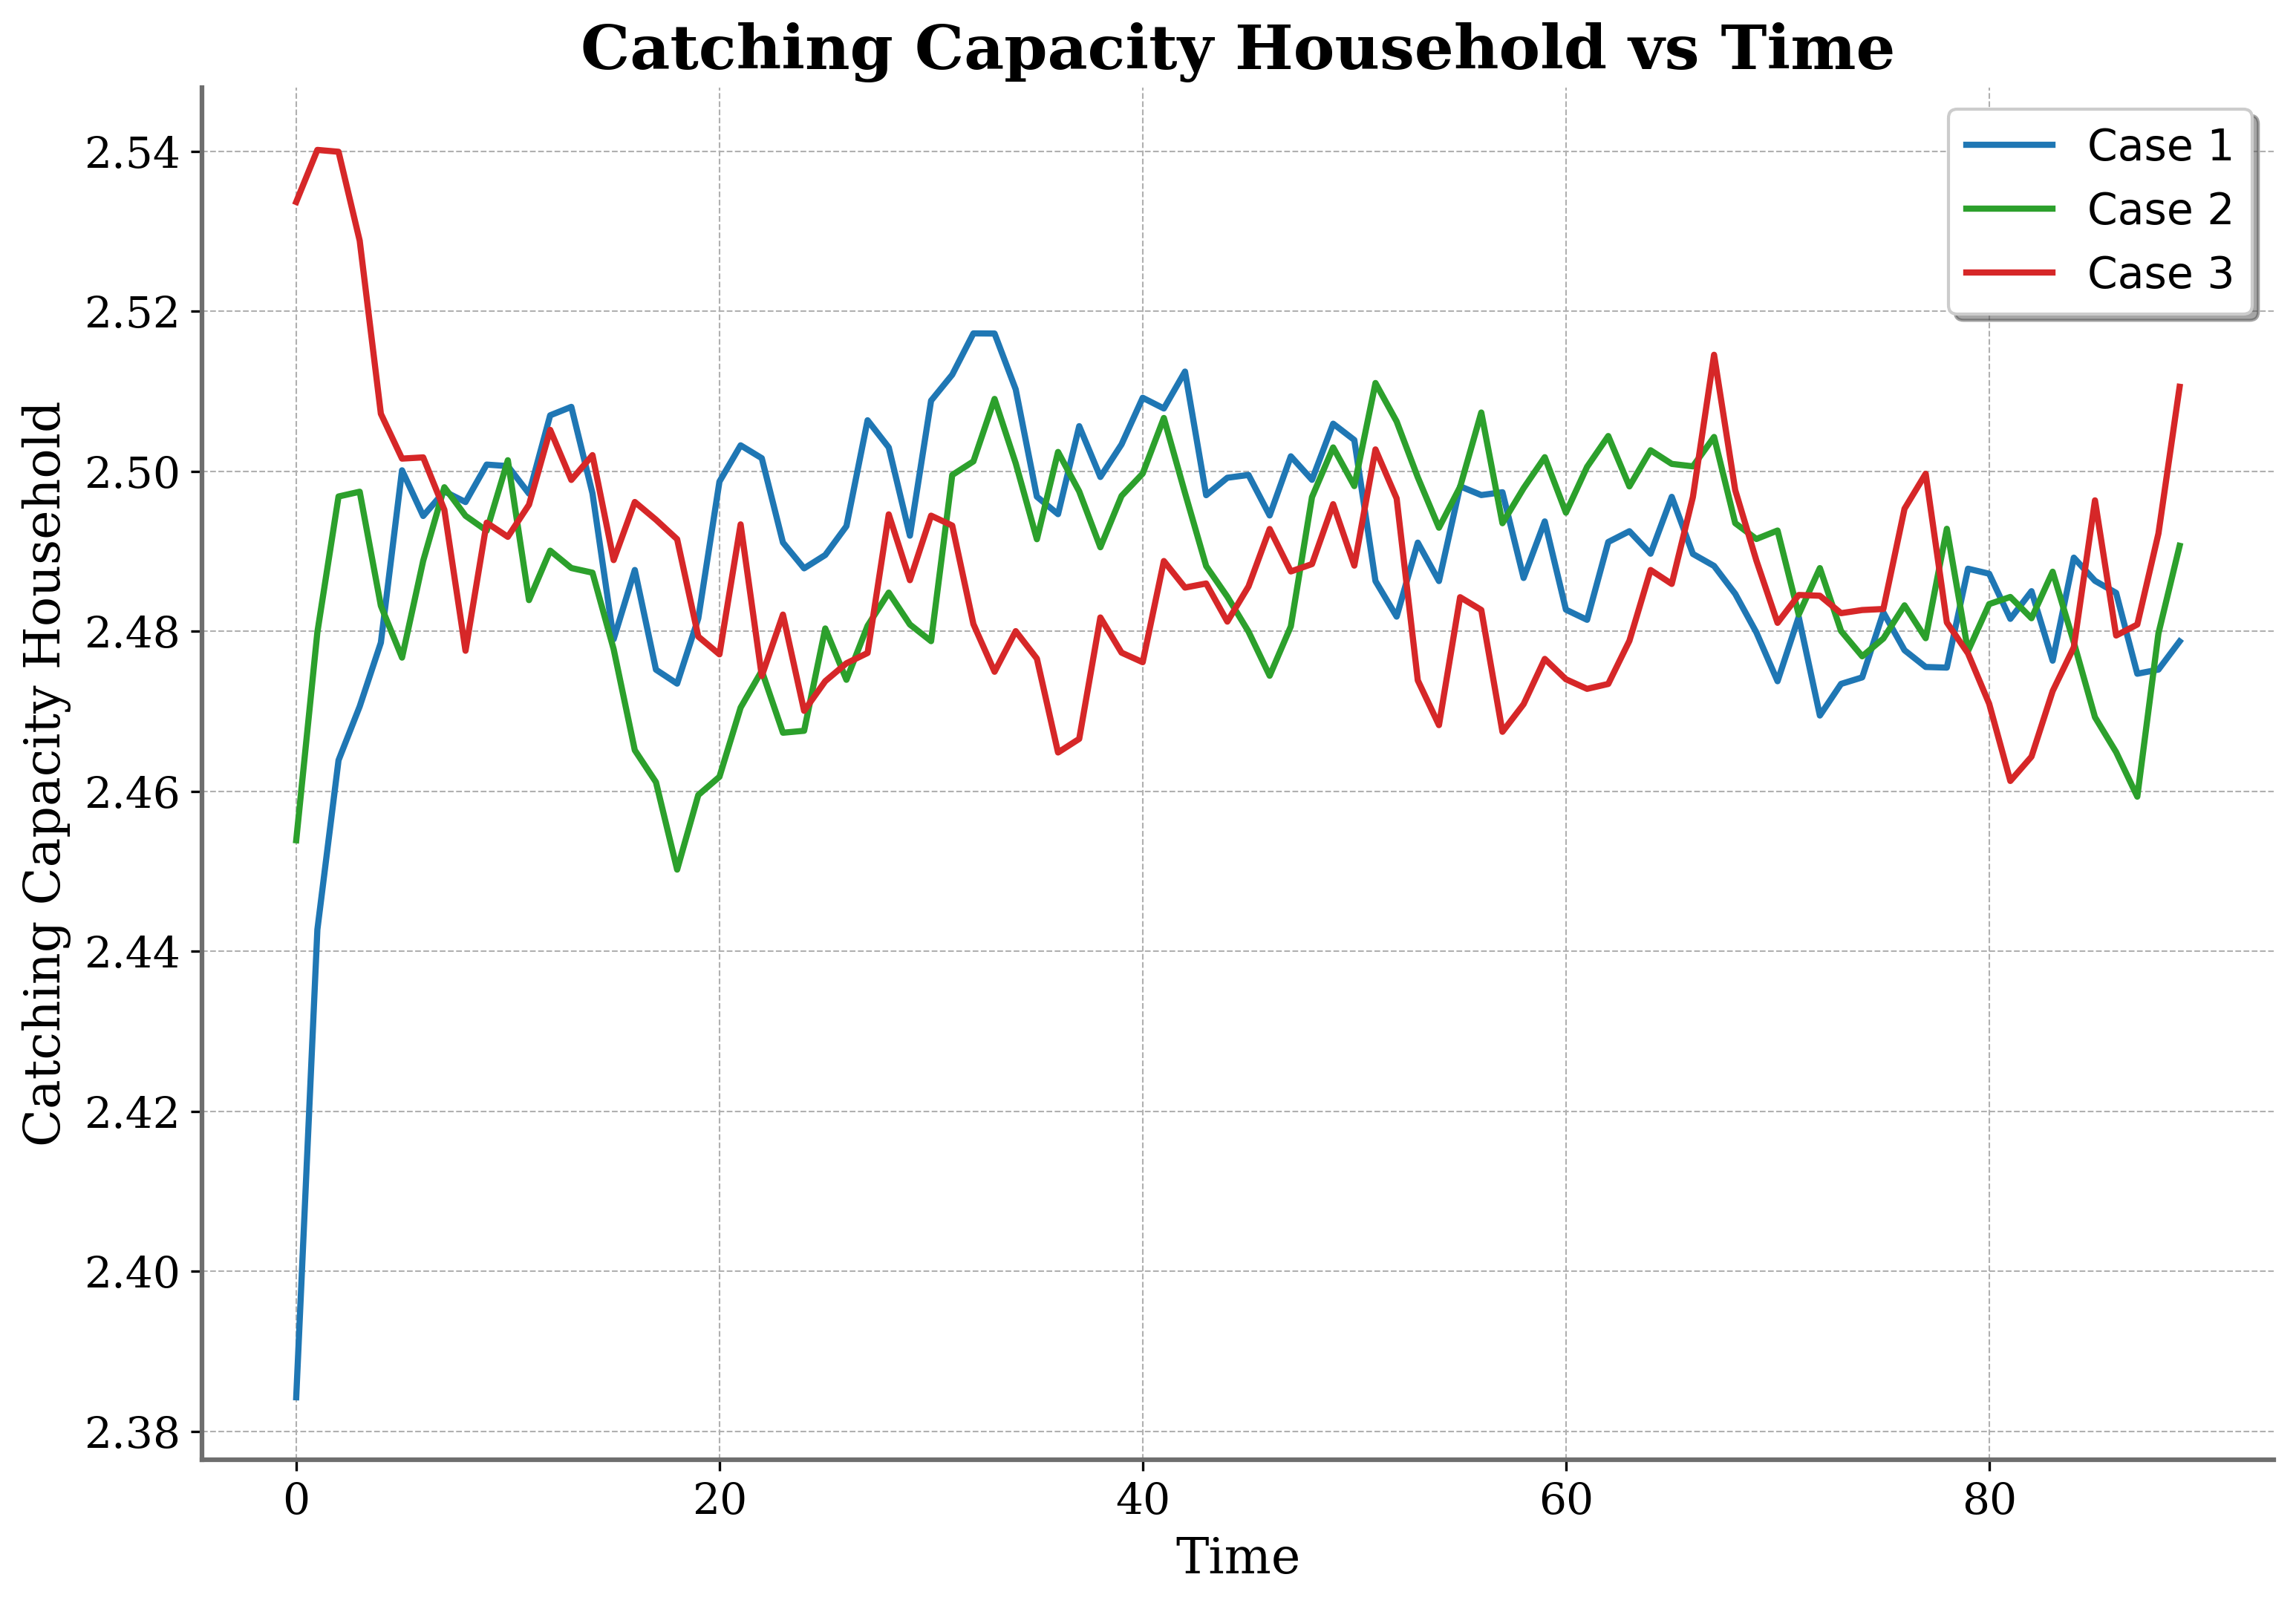
\includegraphics[width=0.4\textwidth]{graph_all/plots_mod/catching_capacity_household_vs_time.png}
    \caption{Catching Capacity Household vs Time}
    \label{fig:catching_household}
\end{figure}
\begin{table}[htbp]
    \centering
    \resizebox{0.4\textwidth}{!}{ % Adjust the 0.9 to control the table size
    \begin{tabular}{lccc}
        \toprule
        \textbf{Statistic} & \textbf{Case 1} & \textbf{Case 2} & \textbf{Case 3} \\
        \midrule
        Mean & 2.489809285 & 2.487280881 & 2.487386642 \\
        Median & 2.49111 & 2.48847 & 2.48499 \\
        Min & 2.38423 & 2.45019 & 2.46128 \\
        Max & 2.51722 & 2.51102 & 2.54016 \\
        Range & 0.13299 & 0.06082 & 0.07888 \\
        Standard Deviation & 0.01741427 & 0.0135165 & 0.01520756 \\
        Variance & 0.00029 & 0.00018 & 0.00023 \\
        Interquartile Range & 0.01781 & 0.01876 & 0.0178 \\
        Skewness & -2.73324 & -0.57742 & 1.33678 \\
        Kurtosis & 14.5607 & -0.22368 & 2.61721 \\
        First Quartile & 2.48165 & 2.47927 & 2.47724 \\
        Third Quartile & 2.49947 & 2.49803 & 2.49503 \\
        MAD & 0.00931 & 0.00947 & 0.00872 \\
        Coefficient of Variation & 0.00688 & 0.00543 & 0.00611 \\
        Mode & 2.38423 & 2.45019 & 2.46128 \\
        \bottomrule
    \end{tabular}
    }
    \caption{Catching Capacity Household - Statistical Analysis}
\end{table}
The study examines household fishers' capacity to catch resources (Figure 12 and Table 12) under moderately regulated circumstances. Case 1 has an average catching capacity of 2.4899, suggesting consistent performance. Case 2 has a lower average but a more compact distribution, suggesting a higher level of stability. Case 3 has the largest range but greater variability, indicating a more stable situation. Case 2 provides the highest level of stability and consistency, while Case 1 is more susceptible to occasional decreases. Case 3 demonstrates greater variability and reduced predictability, suggesting more regulation and oversight. The analysis emphasizes the importance of effectively controlling these variables to ensure consistent performance among families under shifting circumstances.\\
% Sixth figure for Farmers in Loan
\begin{figure}[htbp]
    \centering
    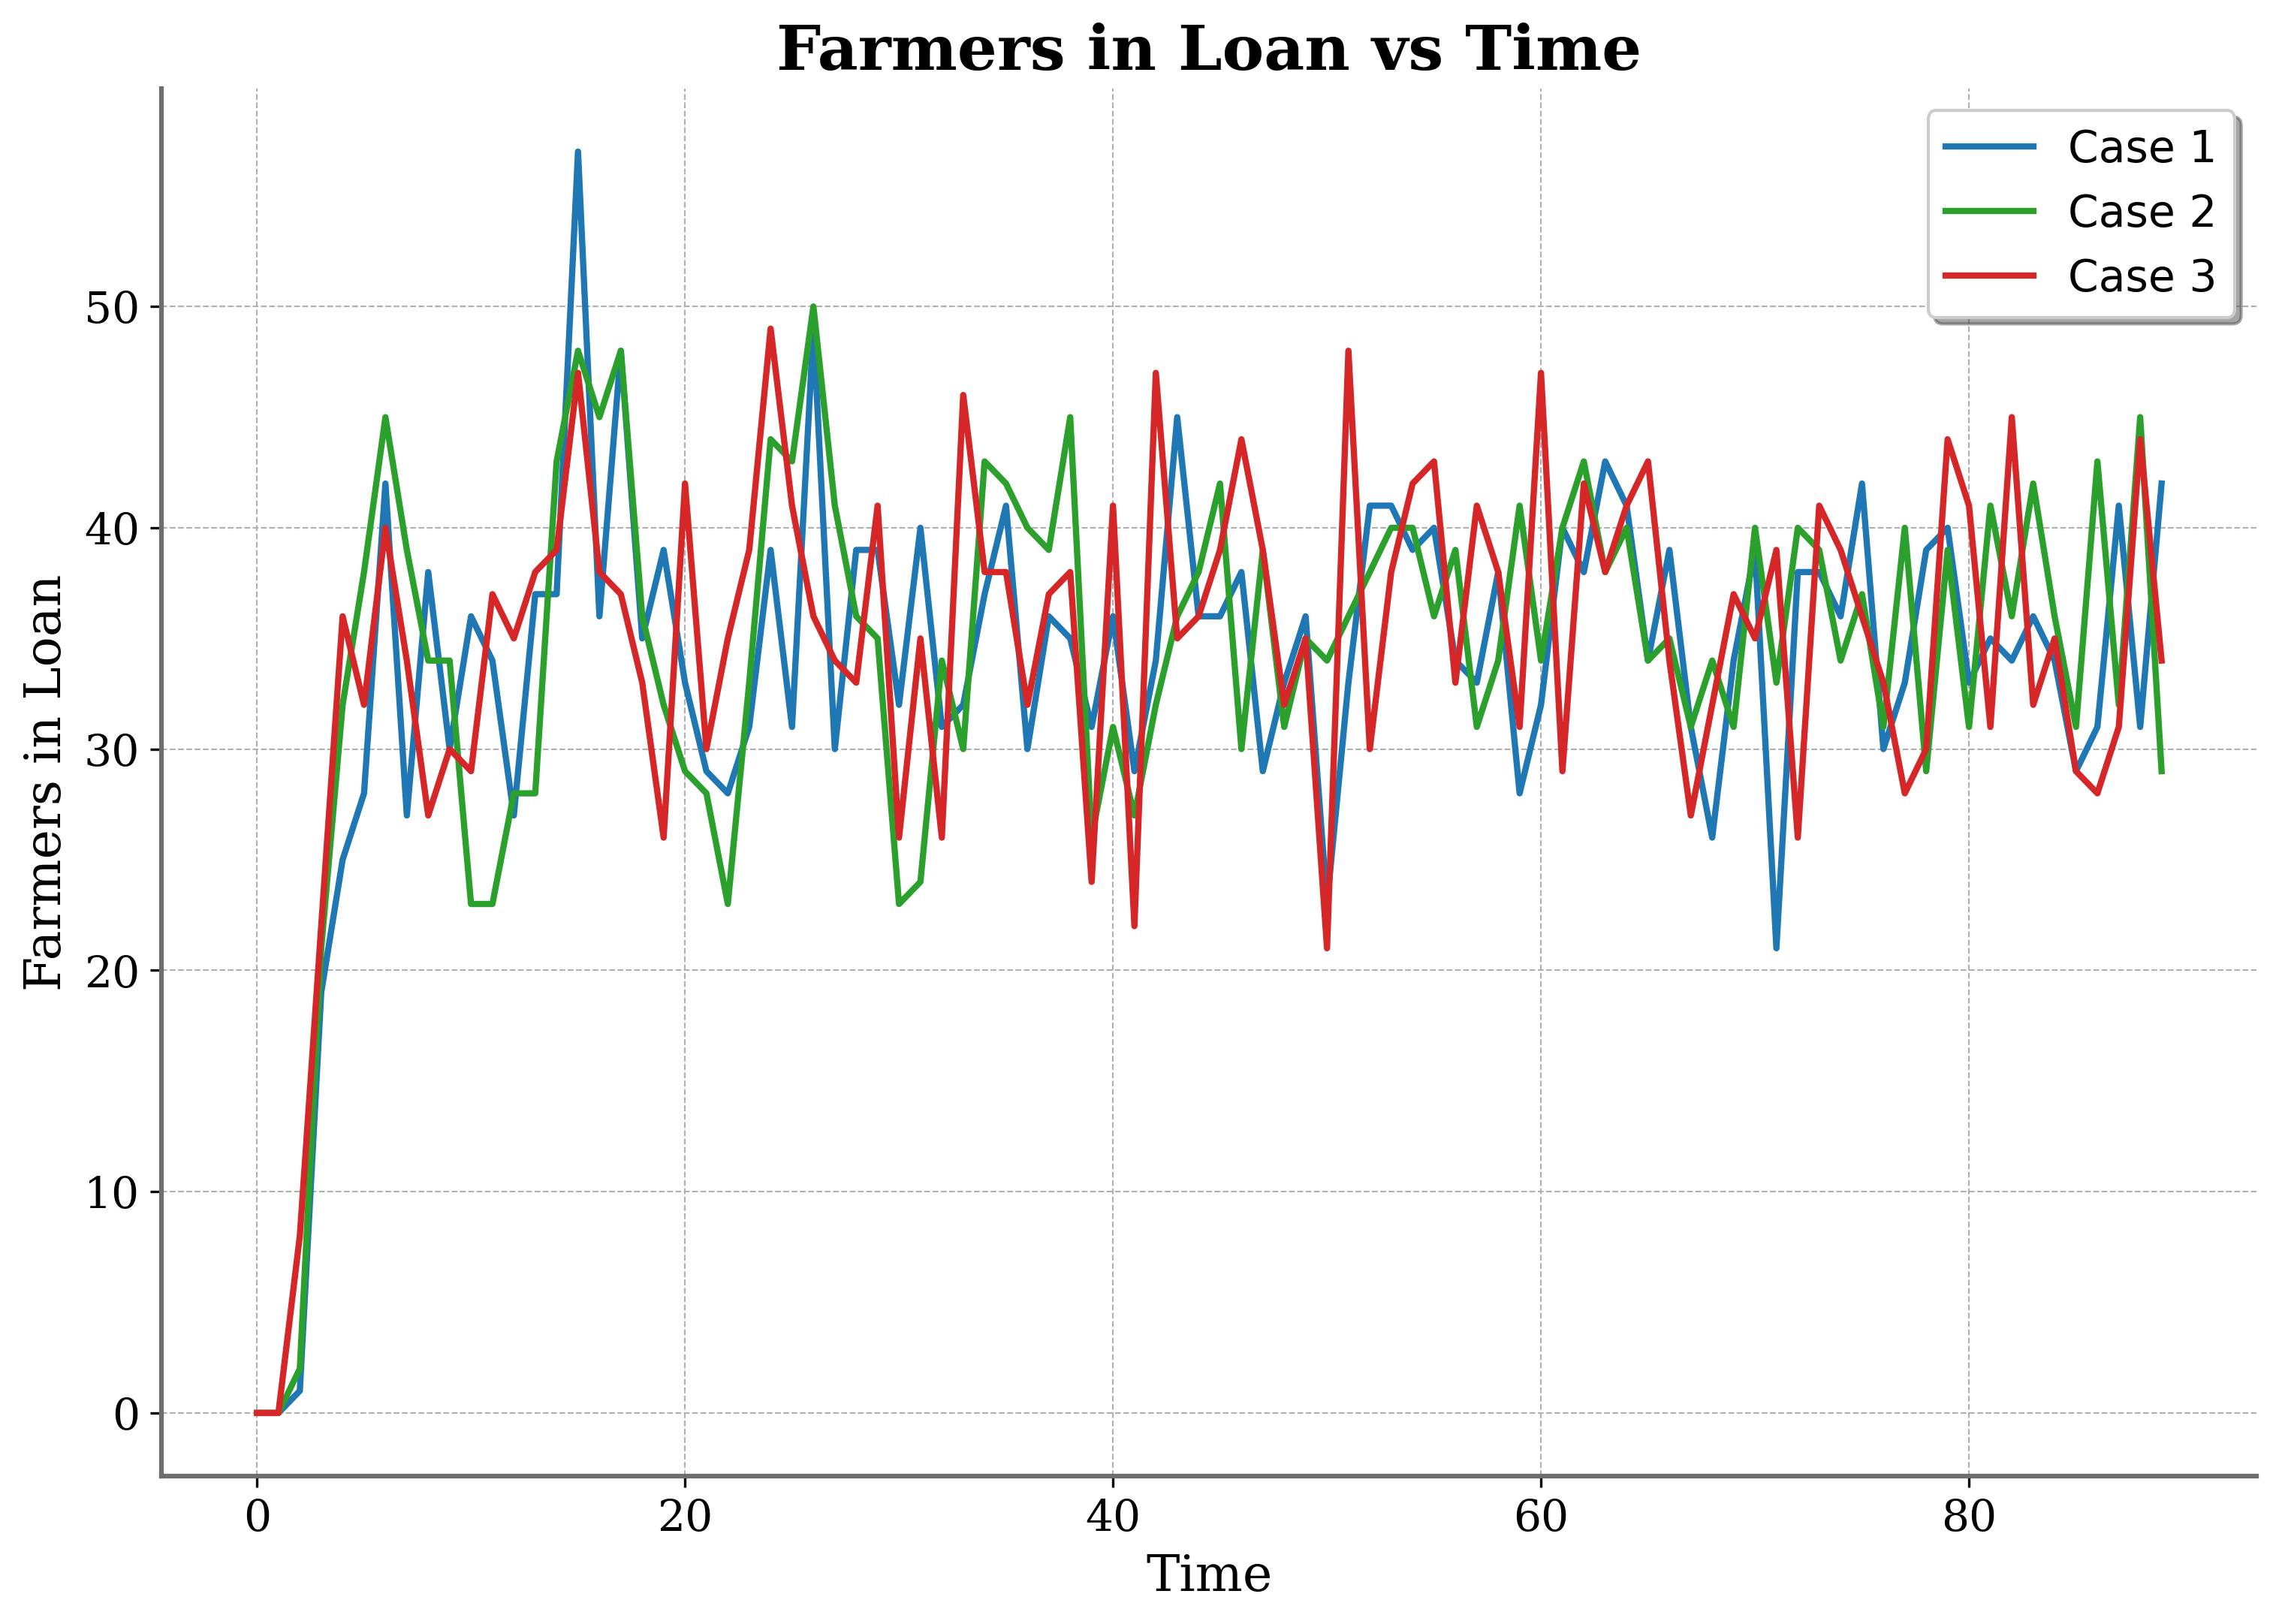
\includegraphics[width=0.4\textwidth]{graph_all/plots_mod/farmers_in_loan_vs_time.png}
    \caption{Farmers in Loan vs Time}
    \label{fig:farmers_loan}
\end{figure}
\begin{table}[htbp]
    \centering
    \resizebox{0.4\textwidth}{!}{ % Adjust the 0.9 to control the table size
    \begin{tabular}{lccc}
        \toprule
        \textbf{Statistic} & \textbf{Case 1} & \textbf{Case 2} & \textbf{Case 3} \\
        \midrule
        Mean & 33.9 & 34.5 & 34.6 \\
        Median & 35 & 35.5 & 35.5 \\
        Min & 0 & 0 & 0 \\
        Max & 57 & 50 & 49 \\
        Range & 57 & 50 & 49 \\
        Standard Deviation & 8.615442211 & 8.87016208 & 8.67101591 \\
        Variance & 74.2258 & 78.6798 & 75.1865 \\
        Interquartile Range & 8 & 9 & 8.75 \\
        Skewness & -1.71413 & -1.74413 & -1.61239 \\
        Kurtosis & 5.99823 & 4.92054 & 4.50774 \\
        First Quartile & 31 & 31 & 31 \\
        Third Quartile & 39 & 40 & 39.75 \\
        MAD & 4 & 4.5 & 4.5 \\
        Coefficient of Variation & 0.25414 & 0.25711 & 0.25061 \\
        Mode & 36 & 34 & 38 \\
        \bottomrule
    \end{tabular}
    }
    \caption{Farmers in Loan - Statistical Analysis}
\end{table}
The study examines farmers' loan participation patterns across three scenarios (Figure 13 and Table 13). In Case 1, the average participation rate is 33.9, with a large range of 57. This indicates erratic borrowing behavior, with low participation levels more prevalent. In Case 2, the mean participation rate is 34.5, with a moderately balanced distribution. In Case 3, the average participation rate is 34.6, with a narrower range of 49. This indicates a more consistent trend, suggesting greater control over external circumstances. However, the elevated kurtosis and negative skewness in Cases 1 and 2 suggest higher volatility and significant deviations from the average, highlighting the need for stabilizing loan participation patterns among farmers.\\
% Seventh figure for Crop Production Capacity
\begin{figure}[htbp]
    \centering
    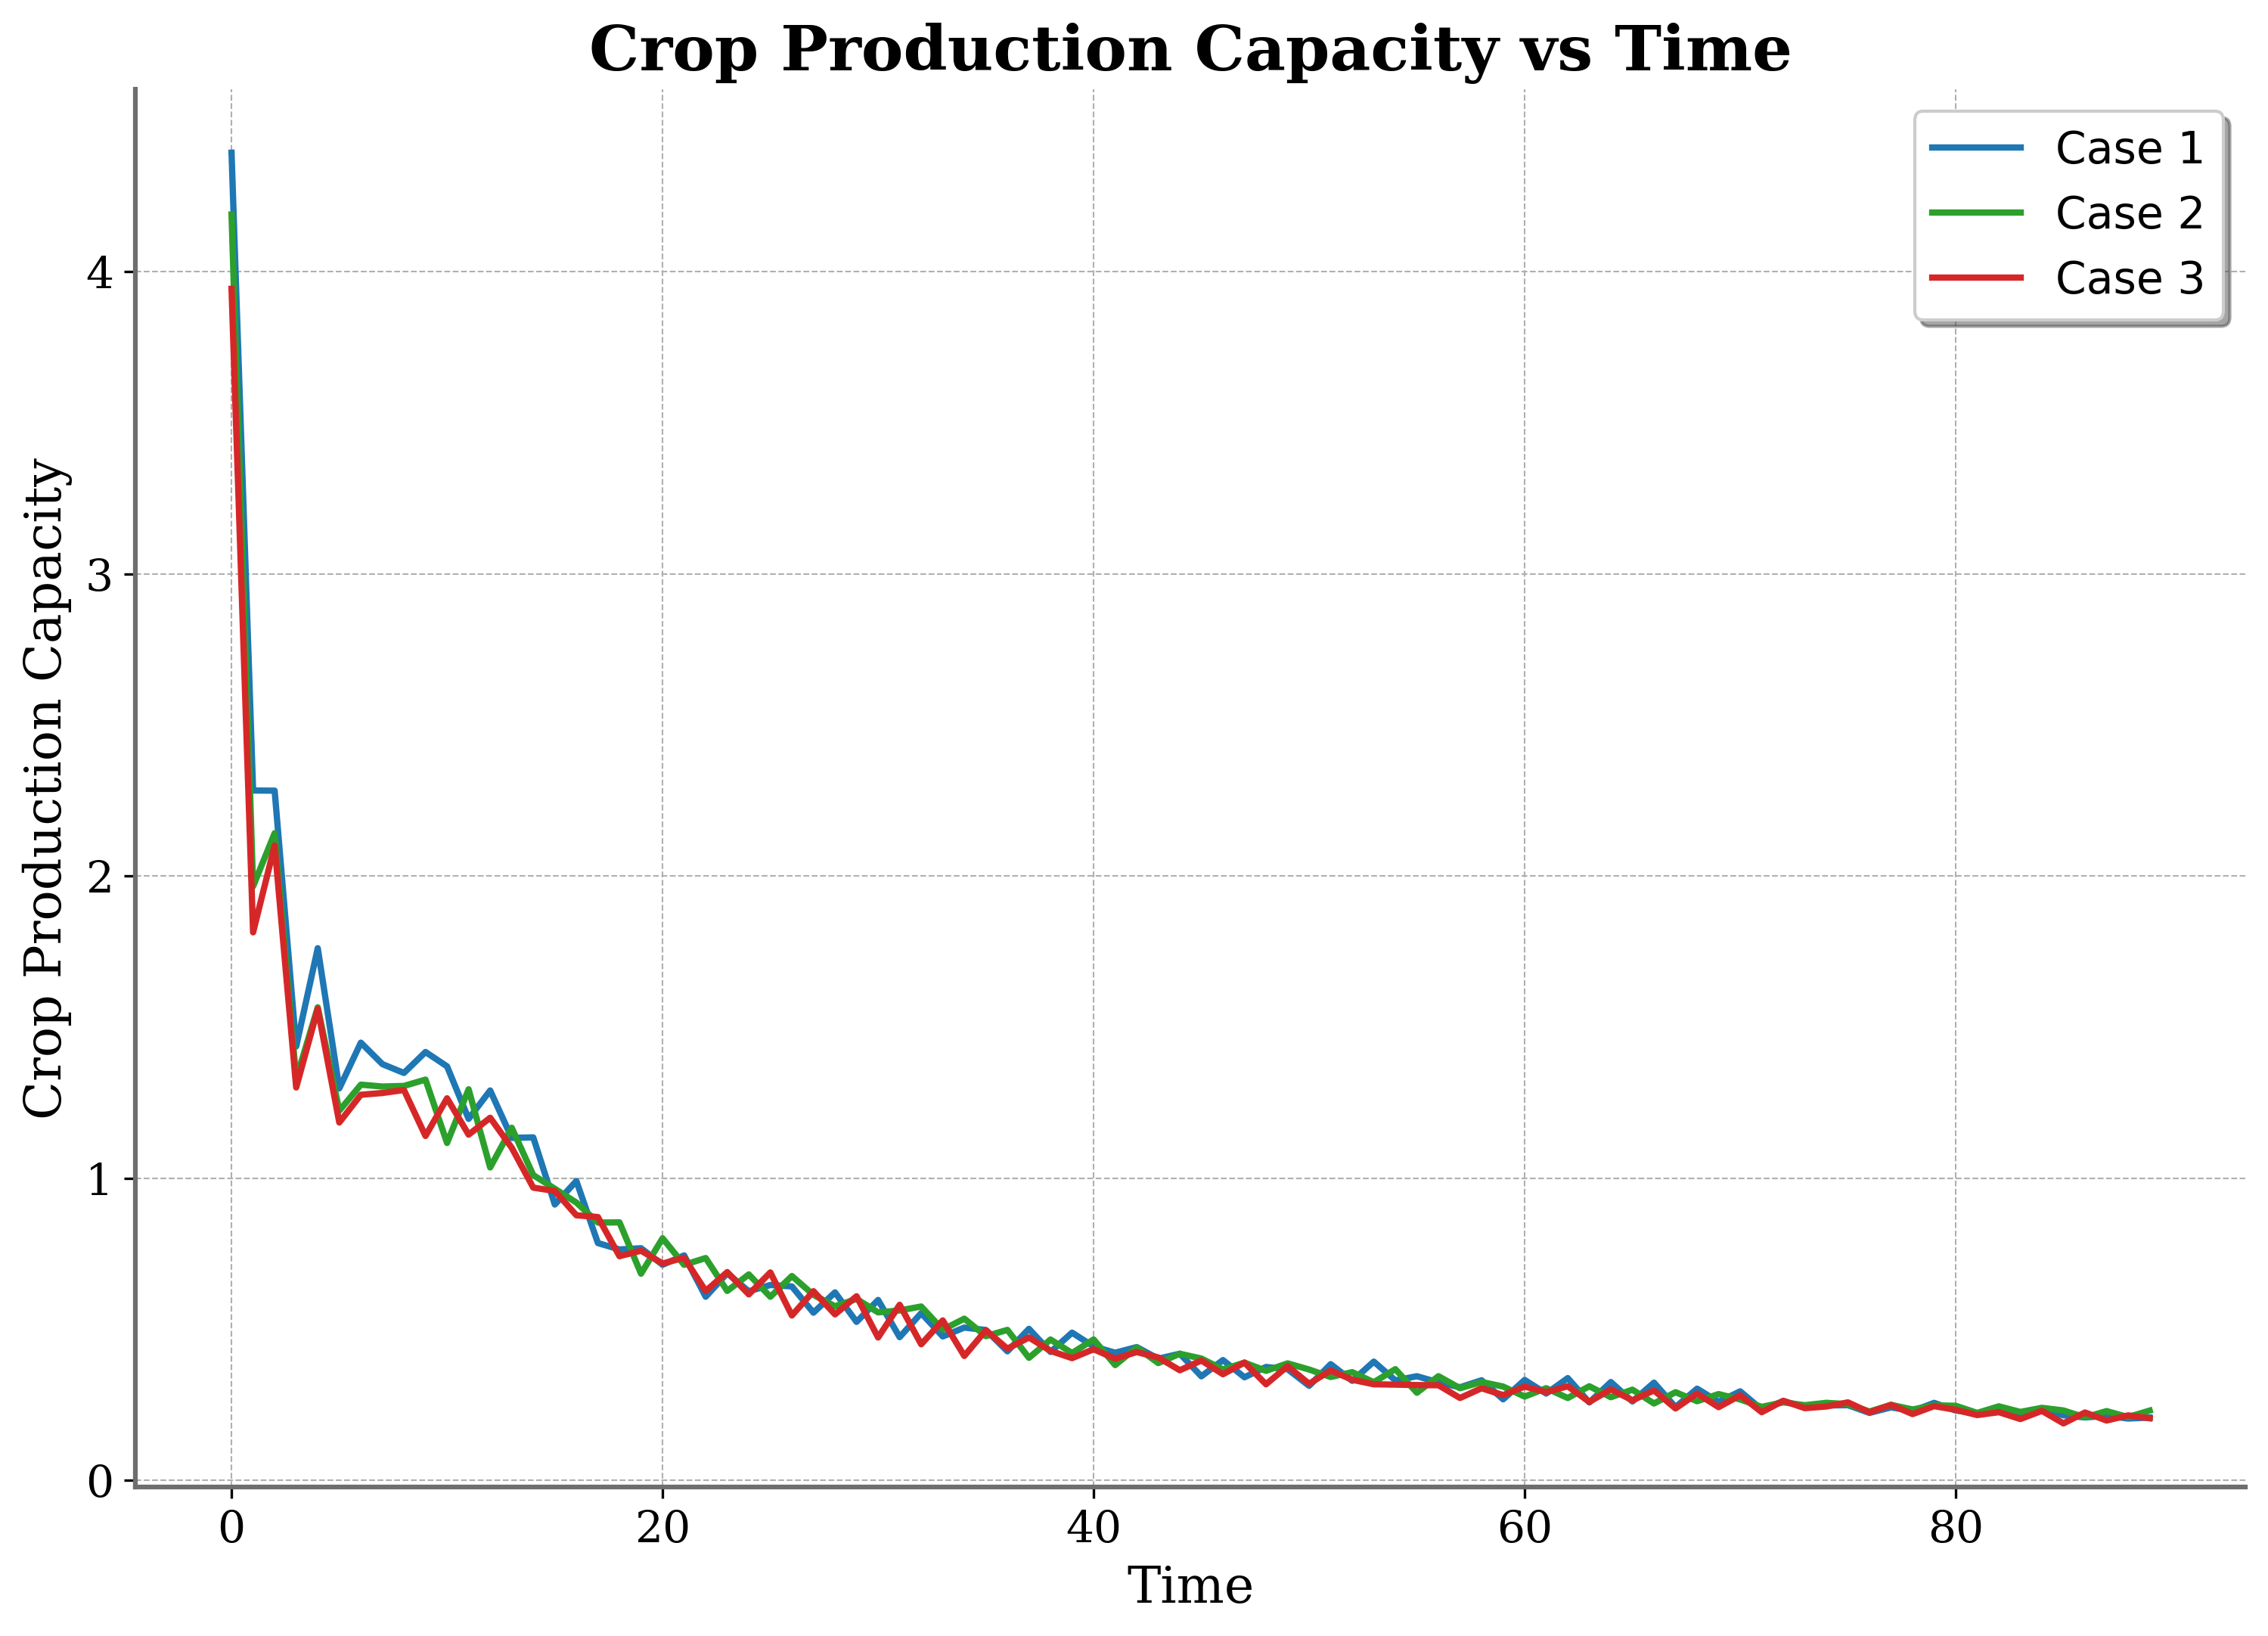
\includegraphics[width=0.4\textwidth]{graph_all/plots_mod/crop_production_capacity_vs_time.png}
    \caption{Crop Production Capacity vs Time}
    \label{fig:crop_production}
\end{figure}
\begin{table}[htbp]
    \centering
    \resizebox{0.4\textwidth}{!}{ % Adjust the 0.9 to control the table size
    \begin{tabular}{lccc}
        \toprule
        \textbf{Statistic} & \textbf{Case 1} & \textbf{Case 2} & \textbf{Case 3} \\
        \midrule
        Mean & 0.6171574 & 0.601116181 & 0.580355928 \\
        Median & 0.4 & 0.38843 & 0.39293 \\
        Min & 0.20417 & 0.20816 & 0.18812 \\
        Max & 4.3932 & 4.18876 & 3.94285 \\
        Range & 4.18903 & 3.98061 & 3.75474 \\
        Standard Deviation & 0.60380355 & 0.55845199 & 0.53477 \\
        Variance & 0.36458 & 0.31187 & 0.28598 \\
        Interquartile Range & 0.41208 & 0.40111 & 0.42225 \\
        Skewness & 3.42627 & 3.54586 & 3.38081 \\
        Kurtosis & 16.151 & 17.8058 & 16.2704 \\
        First Quartile & 0.26317 & 0.27277 & 0.26633 \\
        Third Quartile & 0.67525 & 0.68288 & 0.68858 \\
        MAD & 0.15622 & 0.1448 & 0.15333 \\
        Coefficient of Variation & 0.97836 & 0.92903 & 0.92145 \\
        Mode & 0.20417 & 0.20816 & 0.18812 \\
        \bottomrule
    \end{tabular}
    }
    \caption{Crop Production Capacity - Statistical Analysis}
\end{table}
The study analyses the agricultural production capacity in three different scenarios (Figure 14 and Table 14): Case 1, with an average of 0.617; Case 2, with an average of 0.601; and Case 3, with the lowest average but the highest yield. According to the data, the average crop production capacity declines over time, with Case 3 exhibiting a more consistent and steady trend. Case 1 and 2 have more pronounced fluctuations and abnormalities, suggesting that external factors are responsible for erratic increases in production. The data highlights the significance of efficiently managing significant fluctuations in order to maintain a stable crop production system, particularly in areas that are more prone to unpredictability. The data emphasises the importance of efficiently managing significant fluctuations in order to sustain a stable crop production system.\\
% Force all previous floats to be placed before continuing
\FloatBarrier
\subsubsection{Critical Condition:}
\vspace{0.5cm}
The figures (15-21) and tables (15-21) depict the significant differences in outcomes observed among individuals whose livelihoods depend on critical circumstances compared to those in more favourable and moderate settings. The X-axis remains constant, denoting a single year per unit, whereas the data in each graph covers a time span of up to 90 years.

In this situation, the "Golpata Stock" (shown in Figure 15) experiences a growing level of instability, highlighting the crucial importance of resource management for the Bawali community in handling progressively challenging conditions. Figures 16-17, captioned "Mangrove Fishers in Loan" and "Catching Capacity Mangrove," illustrate the significant challenges encountered by mangrove fishers as they adjust to harsh conditions, characterised by the fluctuating availability of resources over time.

The significance of the plots "Household Fishers in Loan" and "Catching Capacity Household" (Figures 18-19) lies in their ability to accurately depict the challenges faced by household fishers. These graphs exhibit a volatile pattern, suggesting a lack of resources and increasing difficulties in maintaining steady loans and capacity. Furthermore, the statistics presented in Figures 20-21, under "Farmers in Loan" and "Crop Production Capacity," illustrate the difficulties encountered by farmers in adapting to stringent environmental or regulatory constraints, resulting in significant volatility.

The statistical indicators (Tables 15-21) illustrate the heightened volatility in the critical situation in comparison to both the favourable and moderate situations. A comprehensive comparison can be carried out among the three samples by incorporating these markers into the time-series plots. This analysis illustrates the significant disparities observed among the three distinct situations, emphasising that more challenging circumstances result in larger variations, unpredictability, and potential inefficiencies among all the individuals and organisations involved in supporting their livelihoods.\\
% First figure for Bawali
\begin{figure}[htbp]
    \centering
    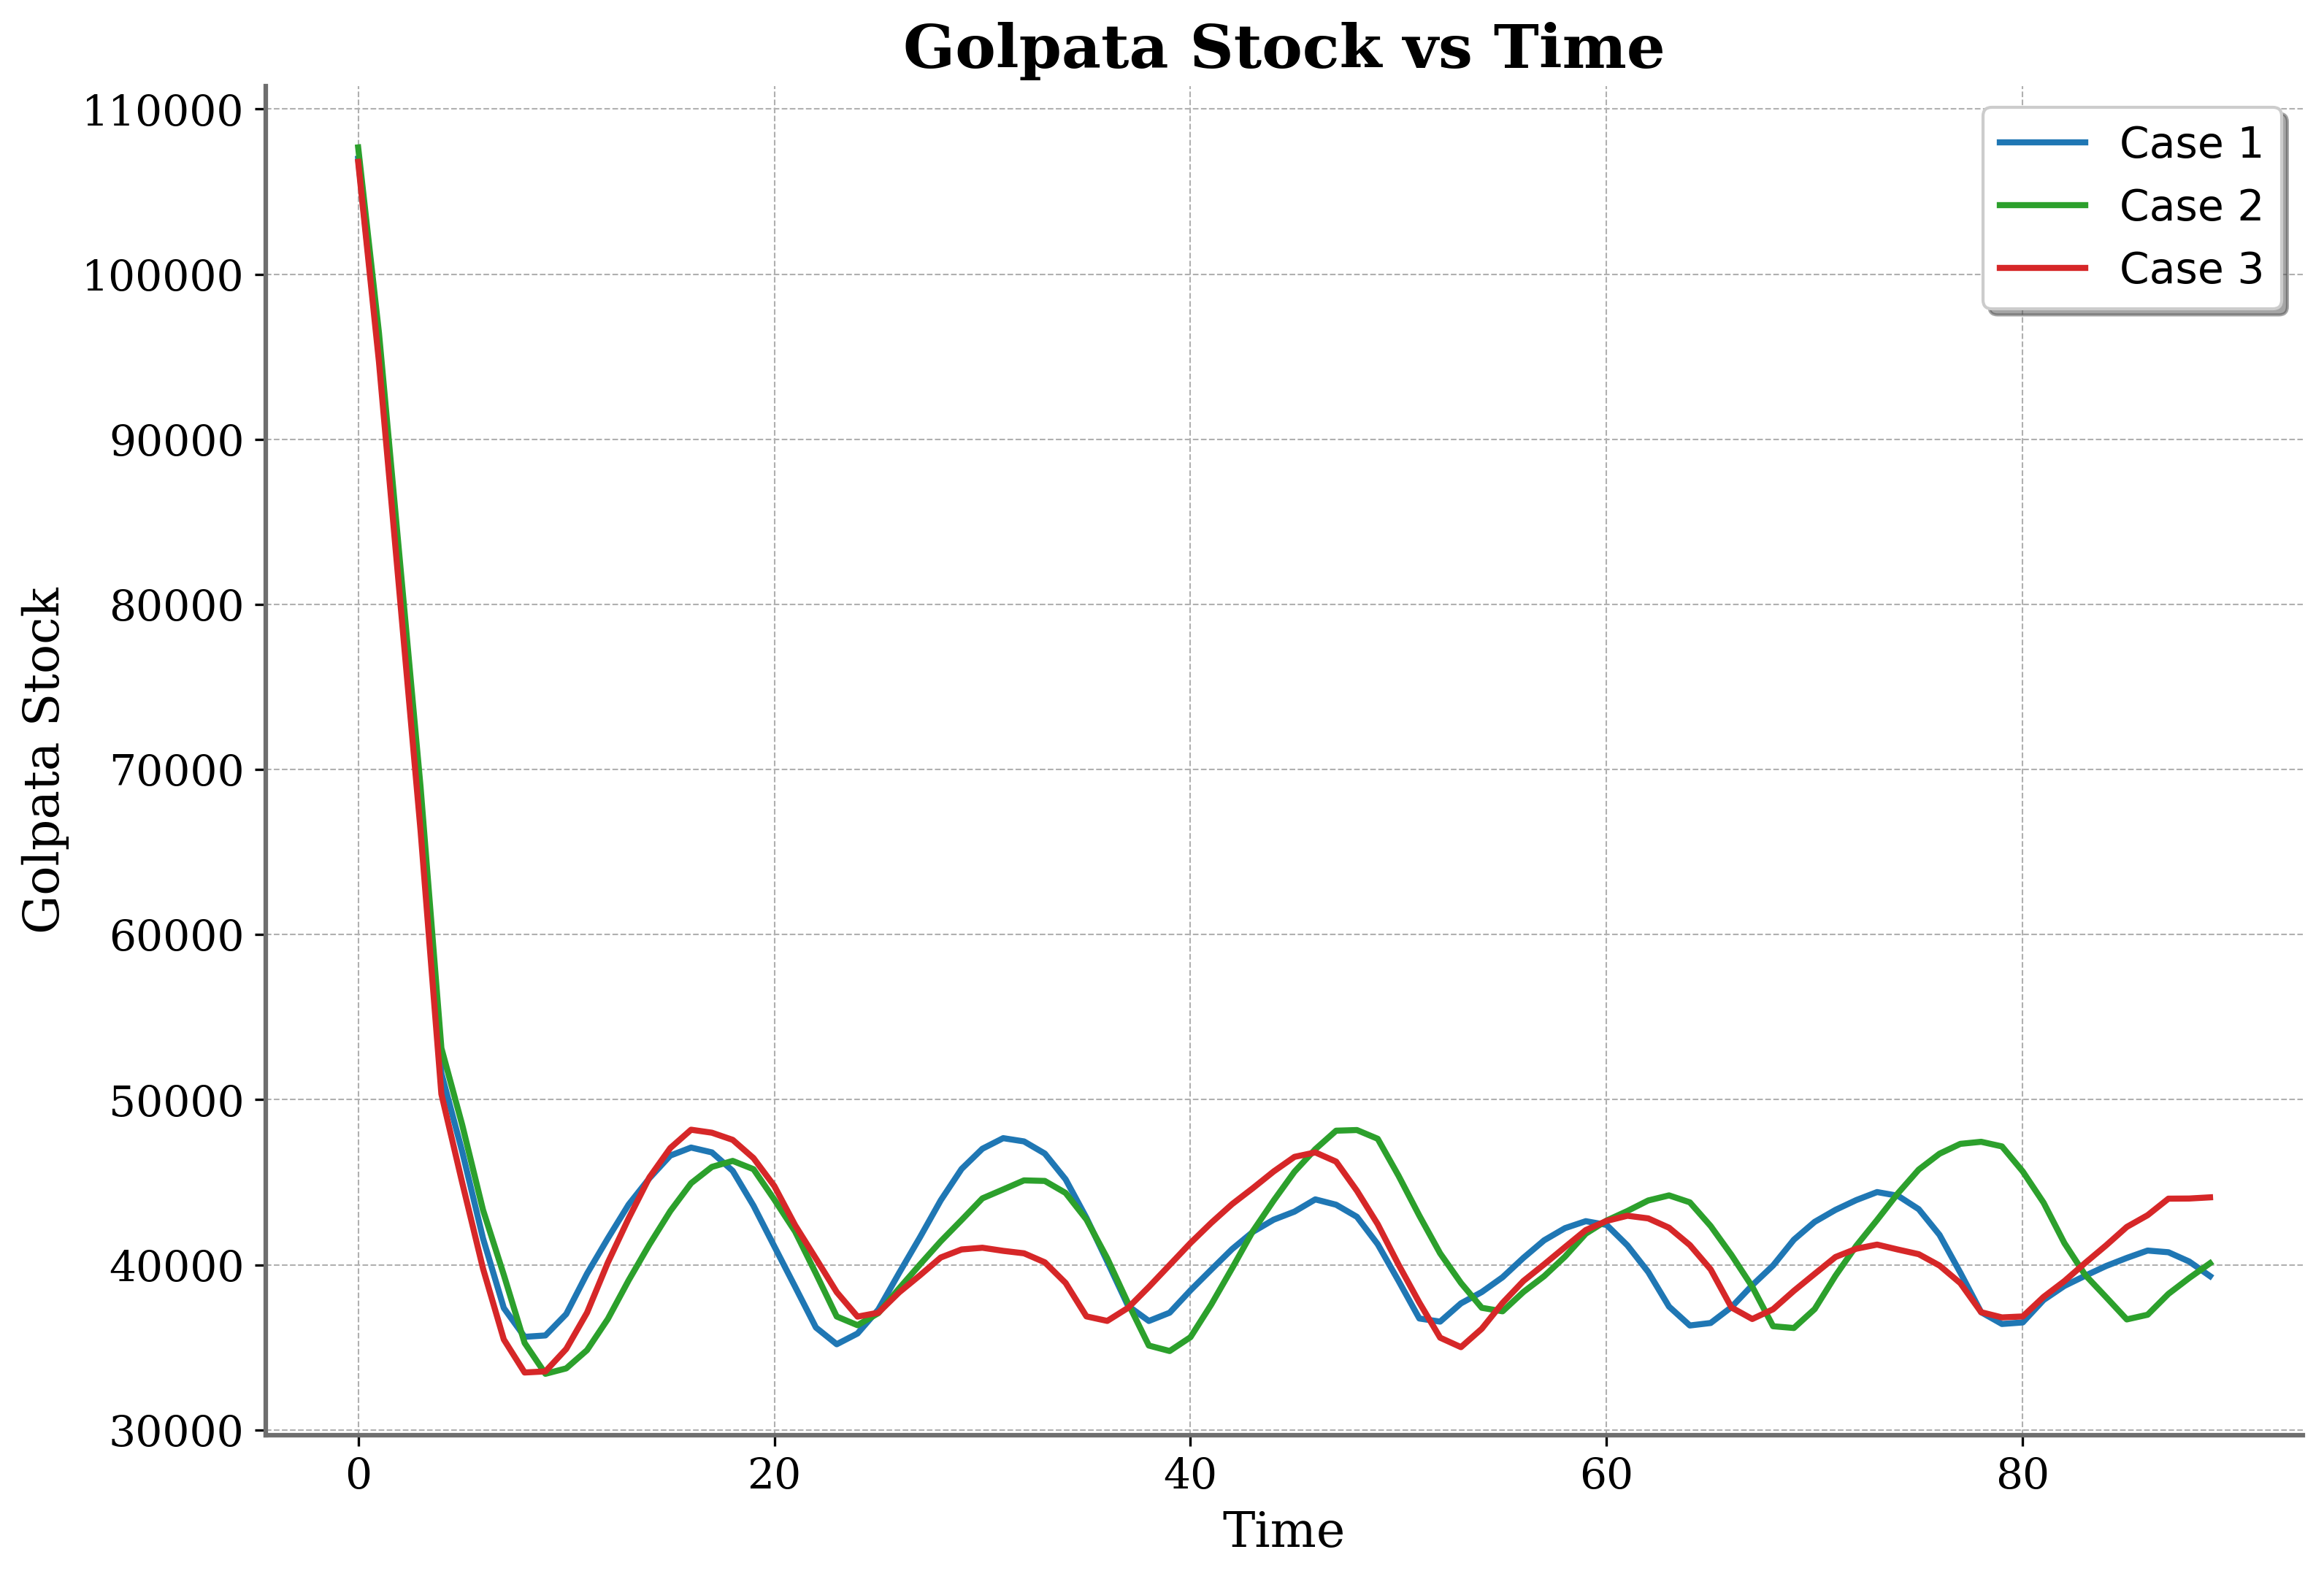
\includegraphics[width=0.4\textwidth]{graph_all/plots_crit/golpata_stock_vs_time.png}
    \caption{Golpata Stock vs Time for Bawali}
    \label{fig:bawali}
\end{figure}
\begin{table}[htbp]
    \centering
    \resizebox{0.4\textwidth}{!}{ % Adjust the 0.9 to control the table size
    \begin{tabular}{lccc}
        \toprule
        \textbf{Statistic} & \textbf{Case 1} & \textbf{Case 2} & \textbf{Case 3} \\
        \midrule
        Mean & 43054.69 & 43572.41 & 42809.87 \\
        Median & 41036.31 & 41950.75 & 40670.86 \\
        Min & 35188.91 & 33399.33 & 33477.98 \\
        Max & 106996.1 & 107681.8 & 106806.8 \\
        Range & 71807.17 & 74282.51 & 73328.82 \\
        Standard Deviation & 10749.5 & 11060.03 & 10714.34 \\
        Variance & 1.16e+08 & 1.22e+08 & 1.15e+08 \\
        Interquartile Range & 5271.708 & 6637.848 & 5172.708 \\
        Skewness & 4.247735 & 3.996843 & 4.245305 \\
        Kurtosis & 19.61752 & 17.92326 & 19.75988 \\
        First Quartile & 38377.03 & 38408.02 & 38335.15 \\
        Third Quartile & 43648.74 & 45045.87 & 43507.86 \\
        MAD & 2650.158 & 3326.655 & 2477.268 \\
        Coefficient of Variation & 0.249671 & 0.253831 & 0.250277 \\
        Mode & 35188.91 & 33399.33 & 33477.98 \\
        \bottomrule
    \end{tabular}
    }
    \caption{Golpata Stock - Statistical Analysis}
\end{table}
The "Golpata Stock vs Time" analysis in critical circumstances (Figure 15 and Table 15) shows significant volatility and fluctuation in resource availability. Cases 1, 2, and 3 show fluctuations between 42,000 and 44,000, indicating growing pressure on resources due to environmental issues or unsustainable extraction methods. The distributions are negatively skewed, with heavy tails, suggesting a tendency for lower values over time. The Bawali community faces more difficulties due to these variations, highlighting the urgent need for intervention or adaptive solutions.
% Second figure for Mangrove Fishermen
\begin{figure}[htbp]
    \centering
    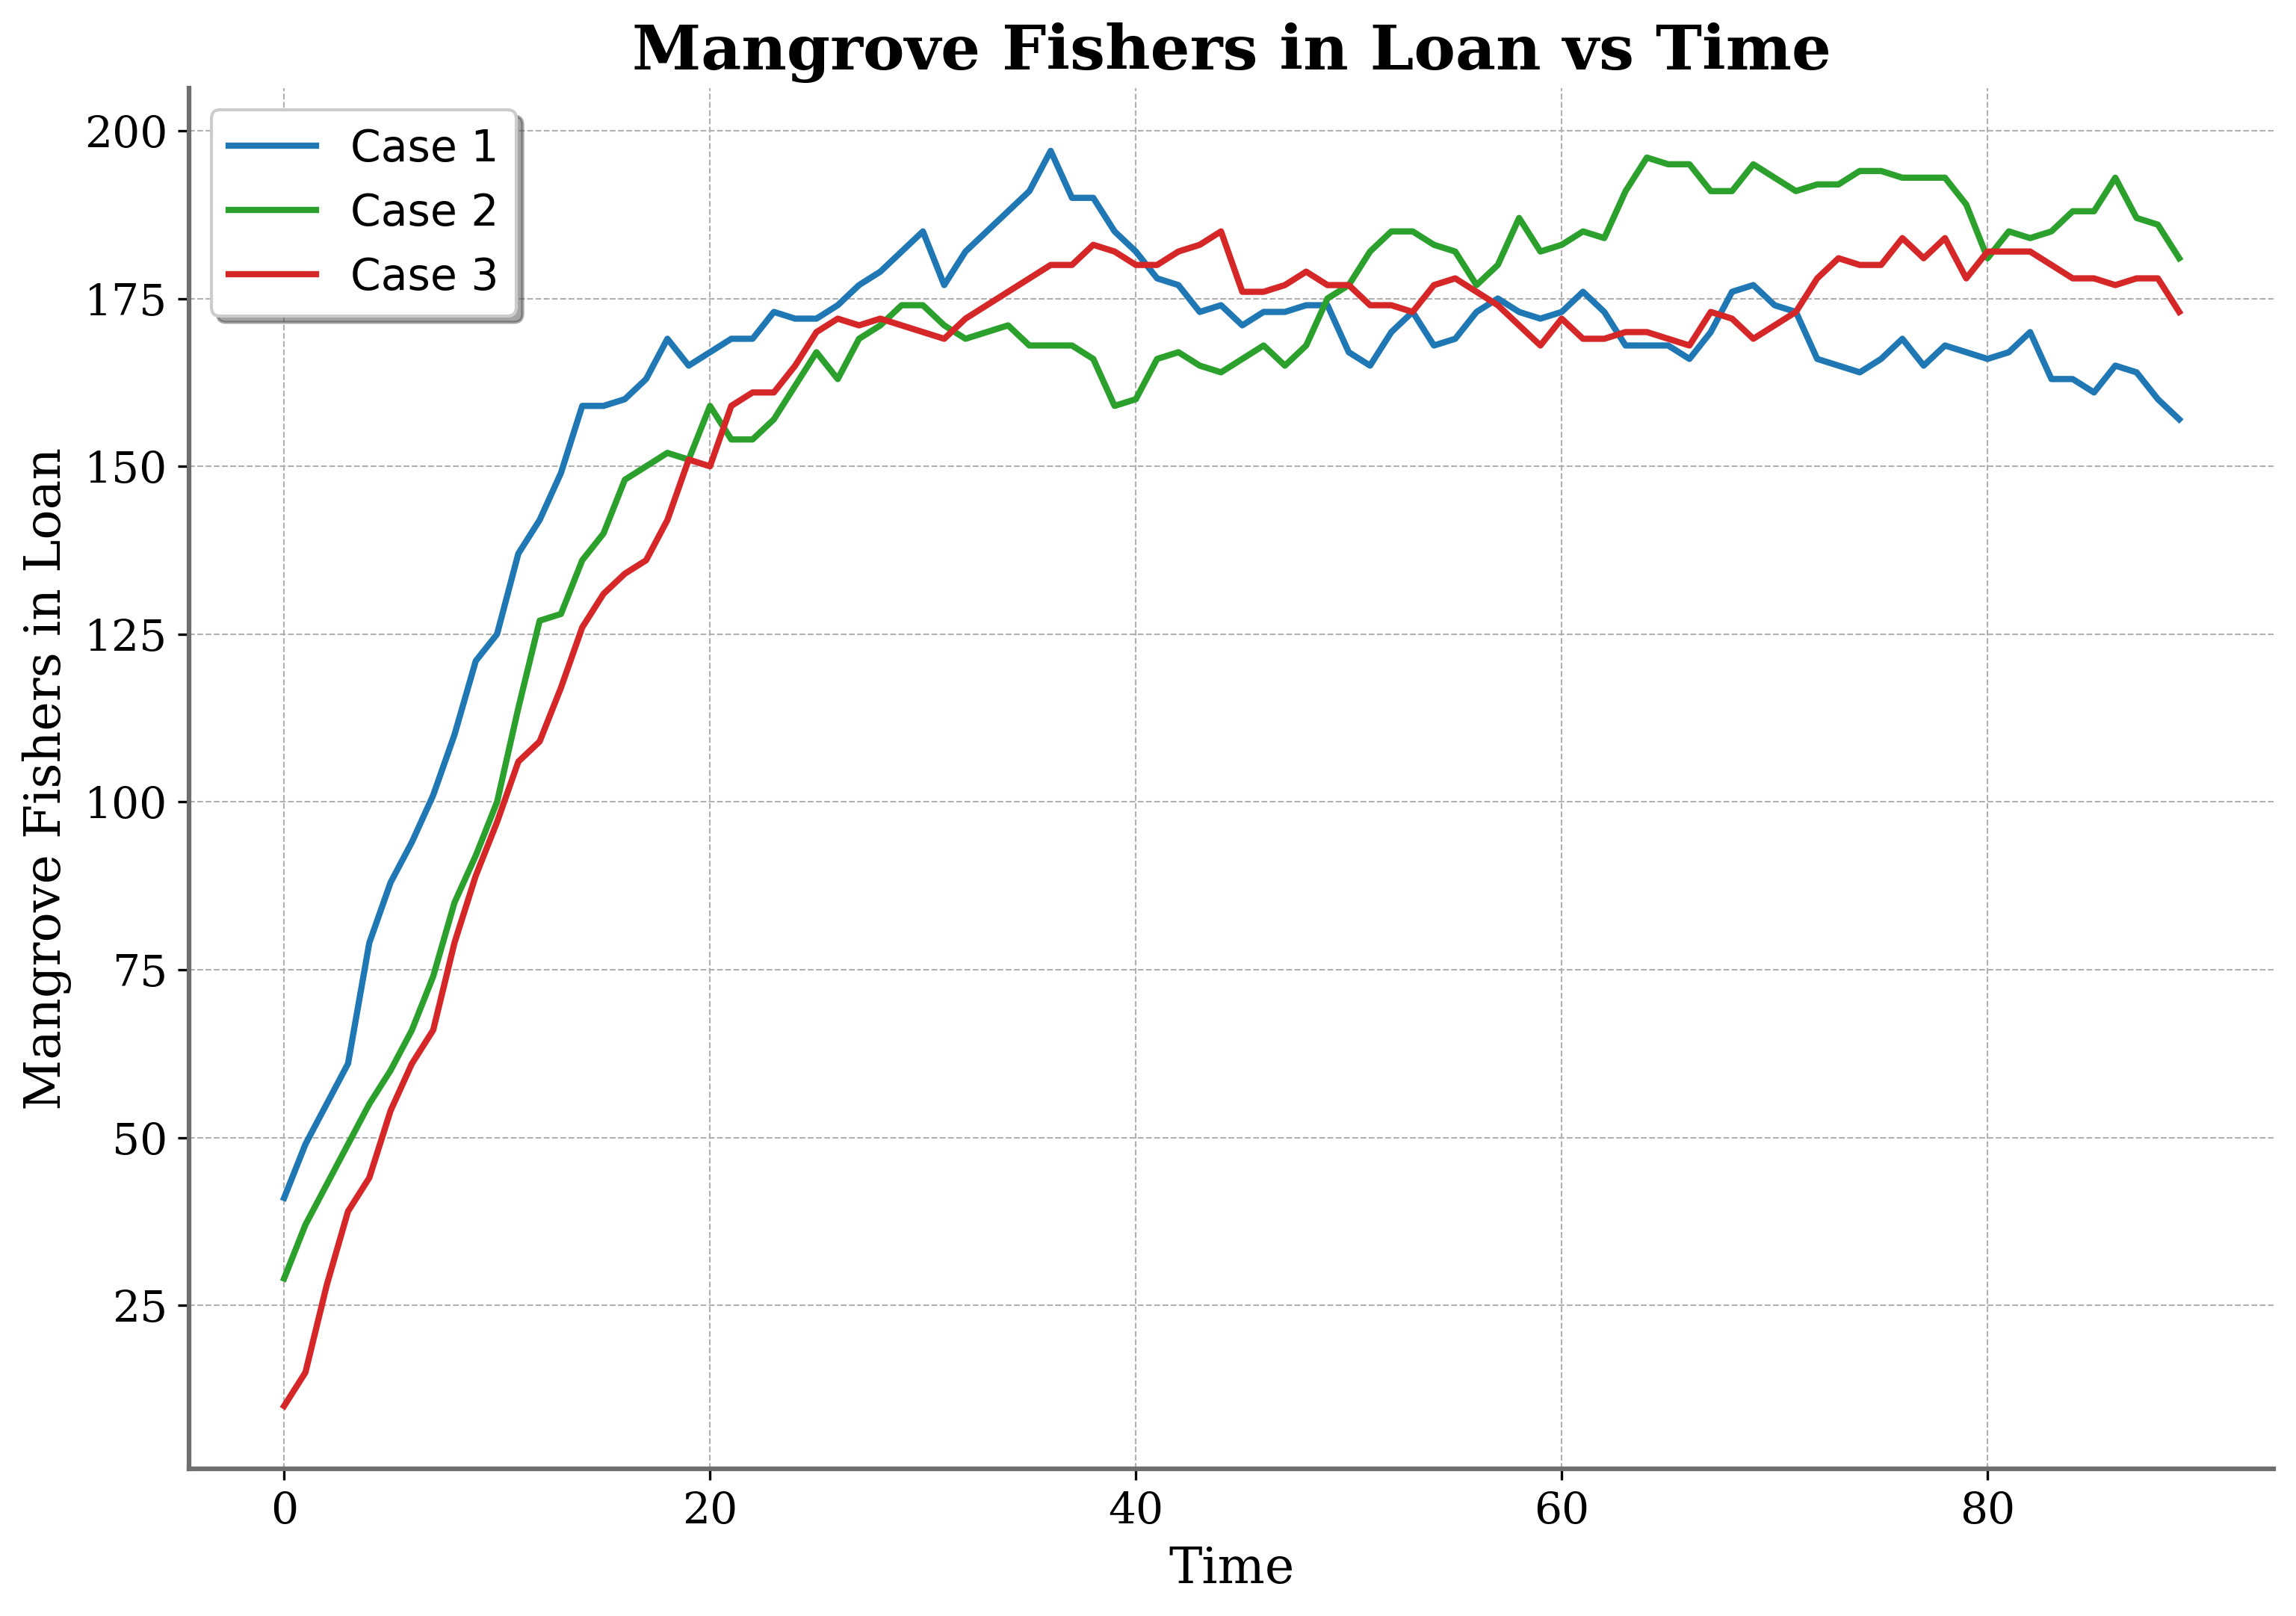
\includegraphics[width=0.4\textwidth]{graph_all/plots_crit/mangrove_fishers_in_loan_vs_time.png}
    \caption{Mangrove Fishers in Loan vs Time}
    \label{fig:mangrove_loan}
\end{figure}
\begin{table}[htbp]
    \centering
    \resizebox{0.4\textwidth}{!}{ % Adjust the 0.9 to control the table size
    \begin{tabular}{lccc}
        \toprule
        \textbf{Statistic} & \textbf{Case 1} & \textbf{Case 2} & \textbf{Case 3} \\
        \midrule
        Mean & 160.1444 & 160.2444 & 155.1778 \\
        Median & 169 & 171 & 172.5 \\
        Min & 41 & 29 & 10 \\
        Max & 197 & 196 & 185 \\
        Range & 156 & 167 & 175 \\
        Standard Deviation & 31.57141 & 40.88001 & 42.59835 \\
        Variance & 996.7542 & 1671.176 & 1814.62 \\
        Interquartile Range & 10.75 & 28.25 & 17 \\
        Skewness & -2.3447 & -1.81838 & -2.04357 \\
        Kurtosis & 4.93113 & 2.409634 & 3.099764 \\
        First Quartile & 163.25 & 157.5 & 161 \\
        Third Quartile & 174 & 185.75 & 178 \\
        MAD & 5 & 14.5 & 6 \\
        Coefficient of Variation & 0.197143 & 0.25511 & 0.274513 \\
        Mode & 173 & 168 & 178 \\
        \bottomrule
    \end{tabular}
    }
    \caption{Mangrove Fishers in Loan - Statistical Analysis}
\end{table}
The study "Mangrove Fishers in Loan vs Time" (Figure 16 and Table 16) reveals significant changes in loan participation patterns among mangrove fishers under challenging circumstances. Cases 1 and 2 show higher levels of loan engagement, while Case 3 shows a more volatile pattern. The study suggests that mangrove fishers are susceptible to heightened stressors and require resilient support structures or adaptive strategies to maintain their livelihoods in challenging settings. The distribution of participation rates is skewed towards lower values.\\
% Third figure for Catching Capacity Mangrove
\begin{figure}[htbp]
    \centering
    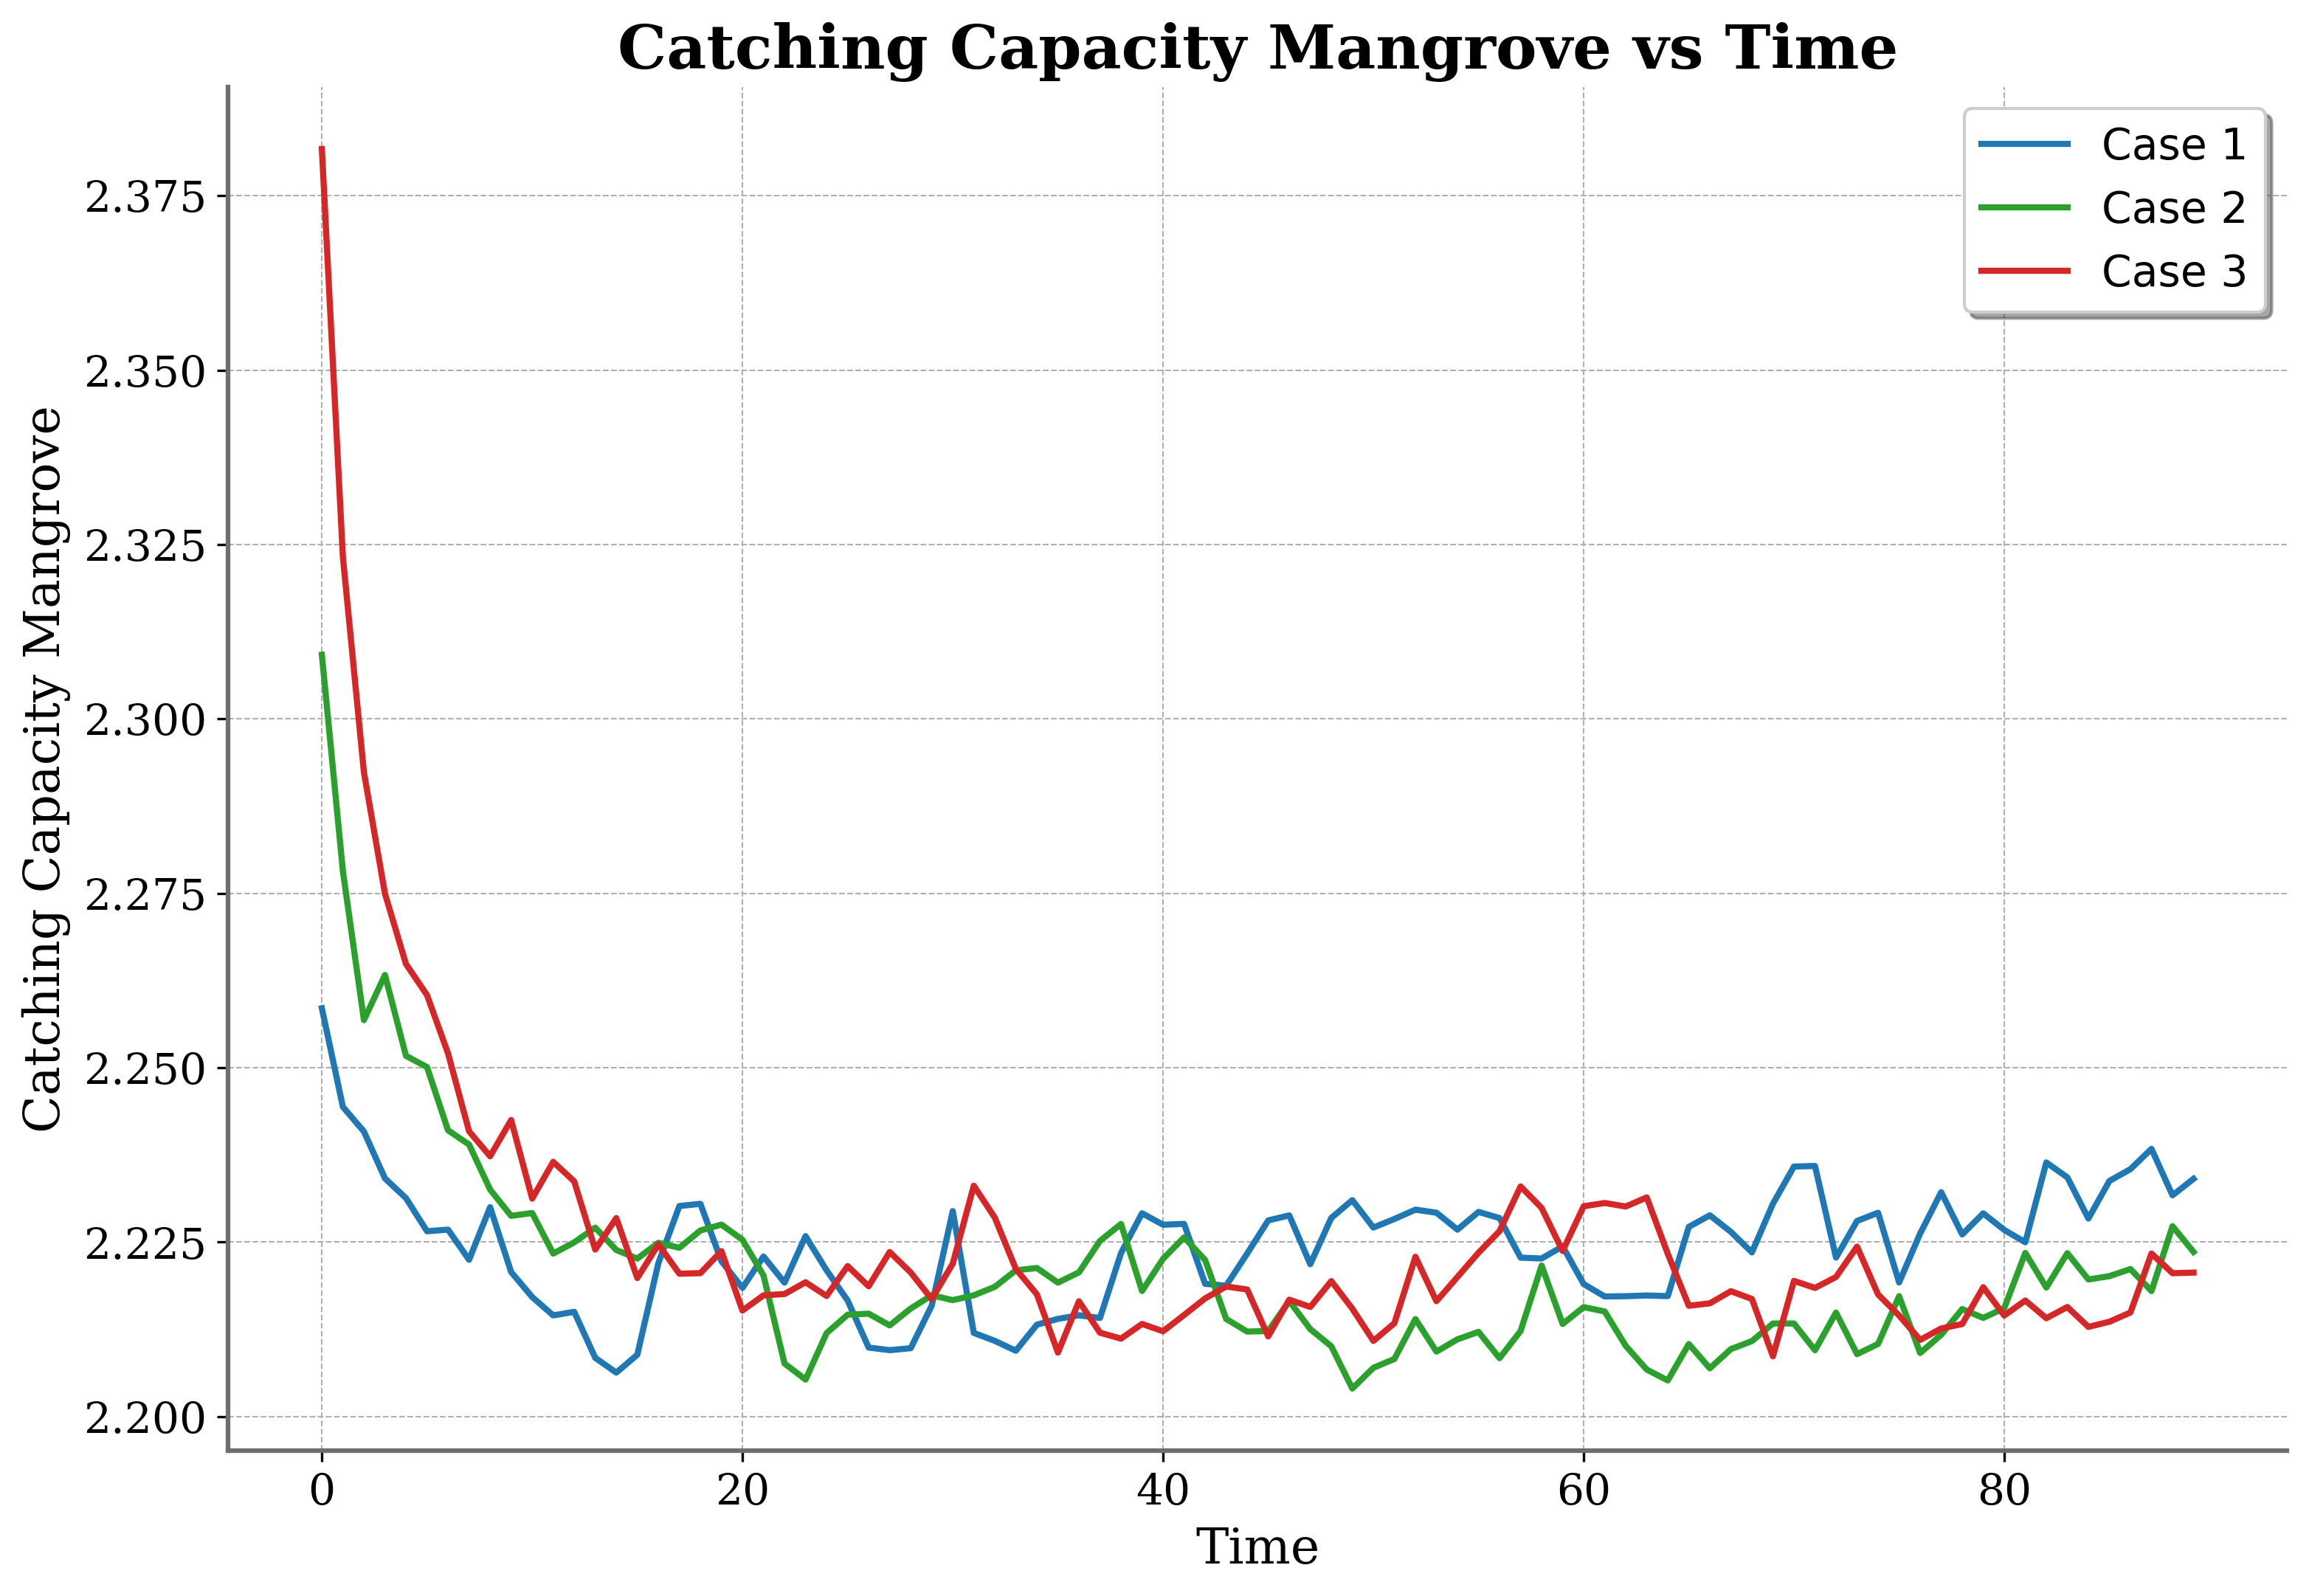
\includegraphics[width=0.4\textwidth]{graph_all/plots_crit/catching_capacity_mangrove_vs_time.png}
    \caption{Catching Capacity Mangrove vs Time}
    \label{fig:catching_mangrove}
\end{figure}
\begin{table}[htbp]
    \centering
    \resizebox{0.4\textwidth}{!}{ % Adjust the 0.9 to control the table size
    \begin{tabular}{lccc}
        \toprule
        \textbf{Statistic} & \textbf{Case 1} & \textbf{Case 2} & \textbf{Case 3} \\
        \midrule
        Mean & 2.224523 & 2.220728 & 2.226036 \\
        Median & 2.226172 & 2.217318 & 2.219434 \\
        Min & 2.206299 & 2.204012 & 2.208632 \\
        Max & 2.258523 & 2.309194 & 2.381691 \\
        Range & 0.052224 & 0.105182 & 0.173059 \\
        Standard Deviation & 0.008823 & 0.015642 & 0.023903 \\
        Variance & 7.78e-05 & 0.000245 & 0.000571 \\
        Interquartile Range & 0.010779 & 0.011659 & 0.010353 \\
        Skewness & 0.403507 & 3.046009 & 4.26585 \\
        Kurtosis & 1.336502 & 12.12983 & 21.58692 \\
        First Quartile & 2.218529 & 2.212151 & 2.215757 \\
        Third Quartile & 2.229307 & 2.22381 & 2.22611 \\
        MAD & 0.004997 & 0.006124 & 0.0044 \\
        Coefficient of Variation & 0.003966 & 0.007043 & 0.010738 \\
        Mode & 2.206299 & 2.204012 & 2.208632 \\
        \bottomrule
    \end{tabular}
    }
    \caption{Catching Capacity Mangrove - Statistical Analysis}
\end{table}
The study reveals a steady decrease in catching capacity of mangrove fishers (Figure 17 and Table 17) in all three scenarios under critical circumstances, typically during stress. Cases 1 and 2 show consistent patterns after a minimum level, while Case 3 shows significant variations over time, indicating unpredictable performance. The mean and median values are similar, but there is significant heterogeneity, particularly in Case 3. The majority of skewness values are positive, suggesting less common but occurring higher-than-average catching capacities. The findings emphasize the need for strategies to decrease variability and ensure consistent results in similar situations.\\
% Fourth figure for Household Fishers in Loan
\begin{figure}[htbp]
    \centering
    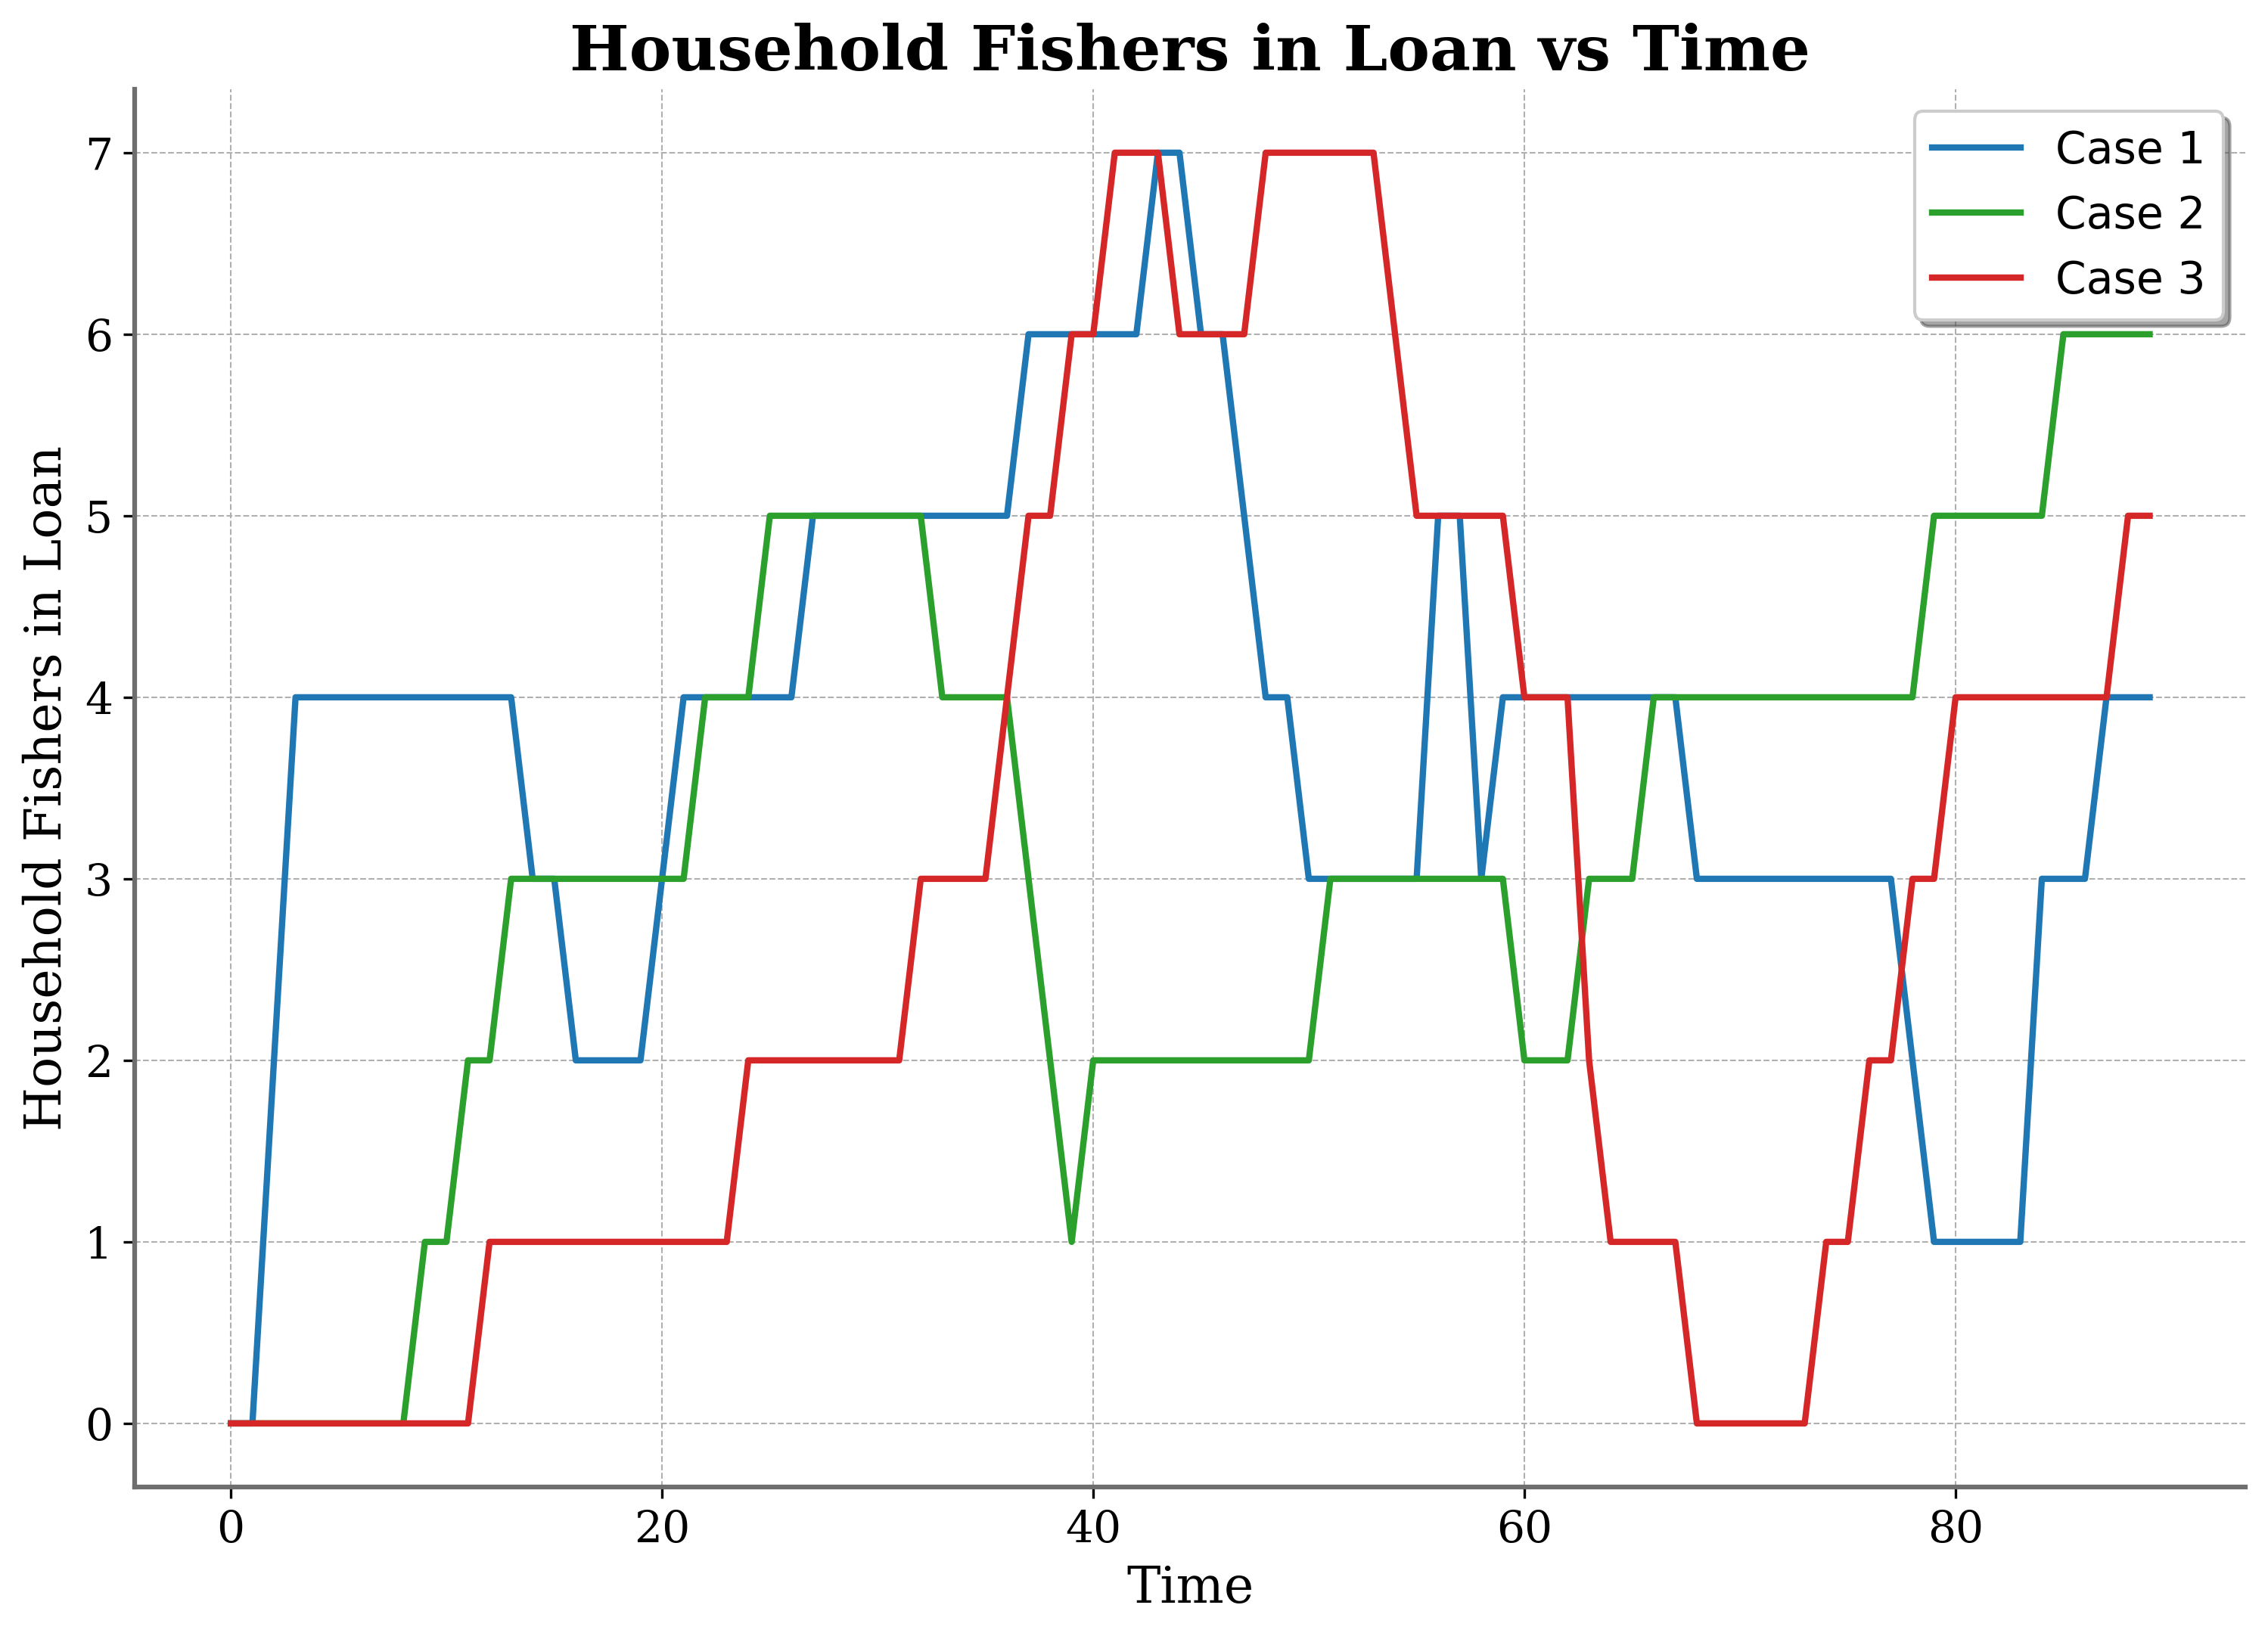
\includegraphics[width=0.4\textwidth]{graph_all/plots_crit/household_fishers_in_loan_vs_time.png}
    \caption{Household Fishers in Loan vs Time}
    \label{fig:household_loan}
\end{figure}
\begin{table}[htbp]
    \centering
    \resizebox{0.4\textwidth}{!}{ % Adjust the 0.9 to control the table size
    \begin{tabular}{lccc}
        \toprule
        \textbf{Statistic} & \textbf{Case 1} & \textbf{Case 2} & \textbf{Case 3} \\
        \midrule
        Mean & 3.744444 & 3.144444 & 2.844444 \\
        Median & 4 & 3 & 2 \\
        Min & 0 & 0 & 0 \\
        Max & 7 & 6 & 7 \\
        Range & 7 & 6 & 7 \\
        Standard Deviation & 1.426563 & 1.604496 & 2.36506 \\
        Variance & 2.035081 & 2.574407 & 5.593508 \\
        Interquartile Range & 1.75 & 2 & 4 \\
        Skewness & -0.24378 & -0.31883 & 0.376365 \\
        Kurtosis & 0.302069 & -0.45993 & -1.18935 \\
        First Quartile & 3 & 2 & 1 \\
        Third Quartile & 4.75 & 4 & 5 \\
        MAD & 1 & 1 & 2 \\
        Coefficient of Variation & 0.380981 & 0.510264 & 0.831466 \\
        Mode & 4 & 3 & 0 \\
        \bottomrule
    \end{tabular}
    }
    \caption{Household Fishers in Loan - Statistical Analysis}
\end{table}
This study investigates the participation of household fishermen in loans during challenging situations (Figure 18 and Table 18), uncovering intermittent patterns and variations in the availability of loans. Case 1 exhibits the greatest average level of involvement, followed by Case 2 and Case 3. The degree of engagement remains consistent, with a maximum rating of 7. Nevertheless, Case 3 exhibits higher levels of inconsistency and instability, leading to more substantial fluctuations in loan participation. The lack of consistency underscores the necessity for more dependable financial institutions to assist family fishers in maintaining uninterrupted access to resources in difficult environments.\\
% Fifth figure for Catching Capacity Household
\begin{figure}[htbp]
    \centering
    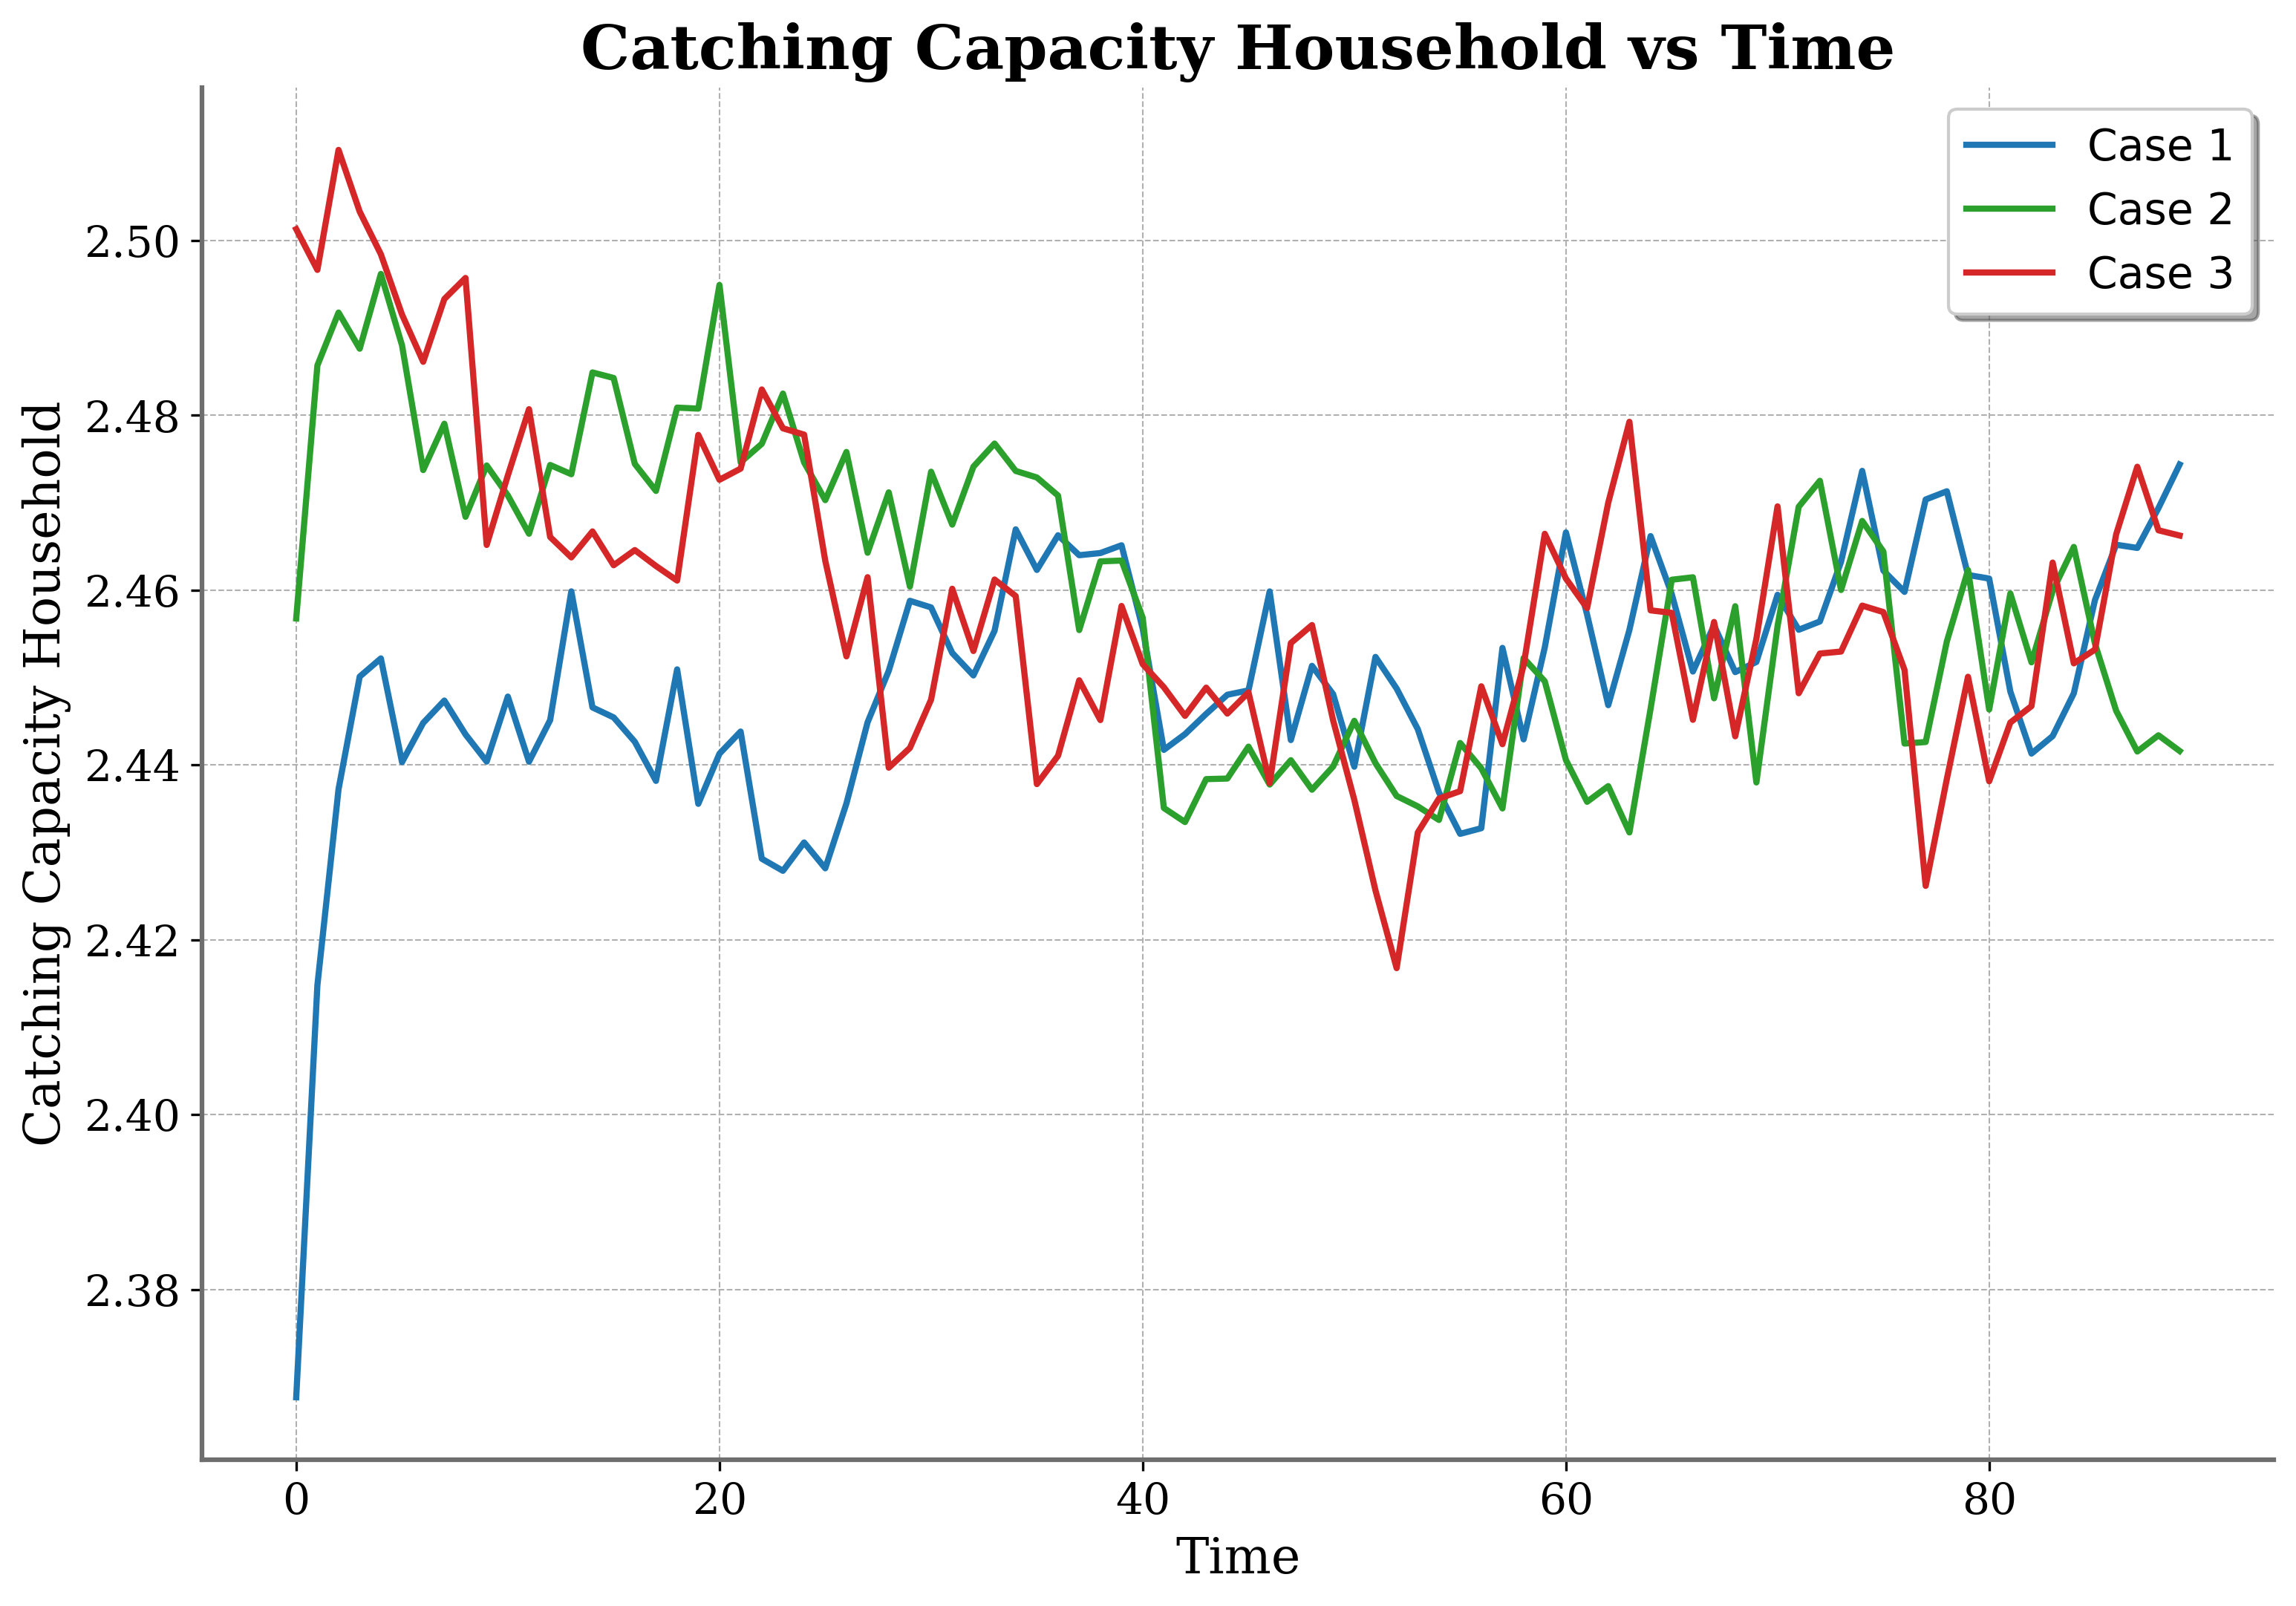
\includegraphics[width=0.4\textwidth]{graph_all/plots_crit/catching_capacity_household_vs_time.png}
    \caption{Catching Capacity Household vs Time}
    \label{fig:catching_household}
\end{figure}
\begin{table}[htbp]
    \centering
    \resizebox{0.4\textwidth}{!}{ % Adjust the 0.9 to control the table size
    \begin{tabular}{lccc}
        \toprule
        \textbf{Statistic} & \textbf{Case 1} & \textbf{Case 2} & \textbf{Case 3} \\
        \midrule
        Mean & 2.449782 & 2.459664 & 2.459043 \\
        Median & 2.450442 & 2.46081 & 2.457455 \\
        Min & 2.367675 & 2.432293 & 2.416768 \\
        Max & 2.474383 & 2.496182 & 2.510369 \\
        Range & 0.106708 & 0.063889 & 0.093601 \\
        Standard Deviation & 0.014493 & 0.017211 & 0.018327 \\
        Variance & 0.00021 & 0.000296 & 0.000336 \\
        Interquartile Range & 0.016505 & 0.031145 & 0.019729 \\
        Skewness & -2.05334 & -1.10841 & 0.328376 \\
        Kurtosis & 9.896711 & 6.442476 & 2.44693 \\
        First Quartile & 2.443031 & 2.442476 & 2.44693 \\
        Third Quartile & 2.459536 & 2.473621 & 2.466659 \\
        MAD & 0.008392 & 0.014097 & 0.009686 \\
        Coefficient of Variation & 0.005916 & 0.006997 & 0.007453 \\
        Mode & 2.367675 & 2.432293 & 2.416768 \\
        \bottomrule
    \end{tabular}
    }
    \caption{Catching Capacity Household - Statistical Analysis}
\end{table}
The study examines the capacity of household fishers (Figure 19 and Table 19) to maintain catch levels amidst environmental and economic challenges. The results show a regular pattern of oscillations, with notable declines and recoveries, highlighting the dynamic obstacles faced by family fishermen. Case 1 shows greater variability in catch capacity, indicating frequent disruptions or modifications. The data points are concentrated at larger capacity levels, with the highest skewness at -2.05344. The findings emphasize the need for strong support techniques to stabilize catching efforts in turbulent environments.\\
% Sixth figure for Farmers in Loan
\begin{figure}[htbp]
    \centering
    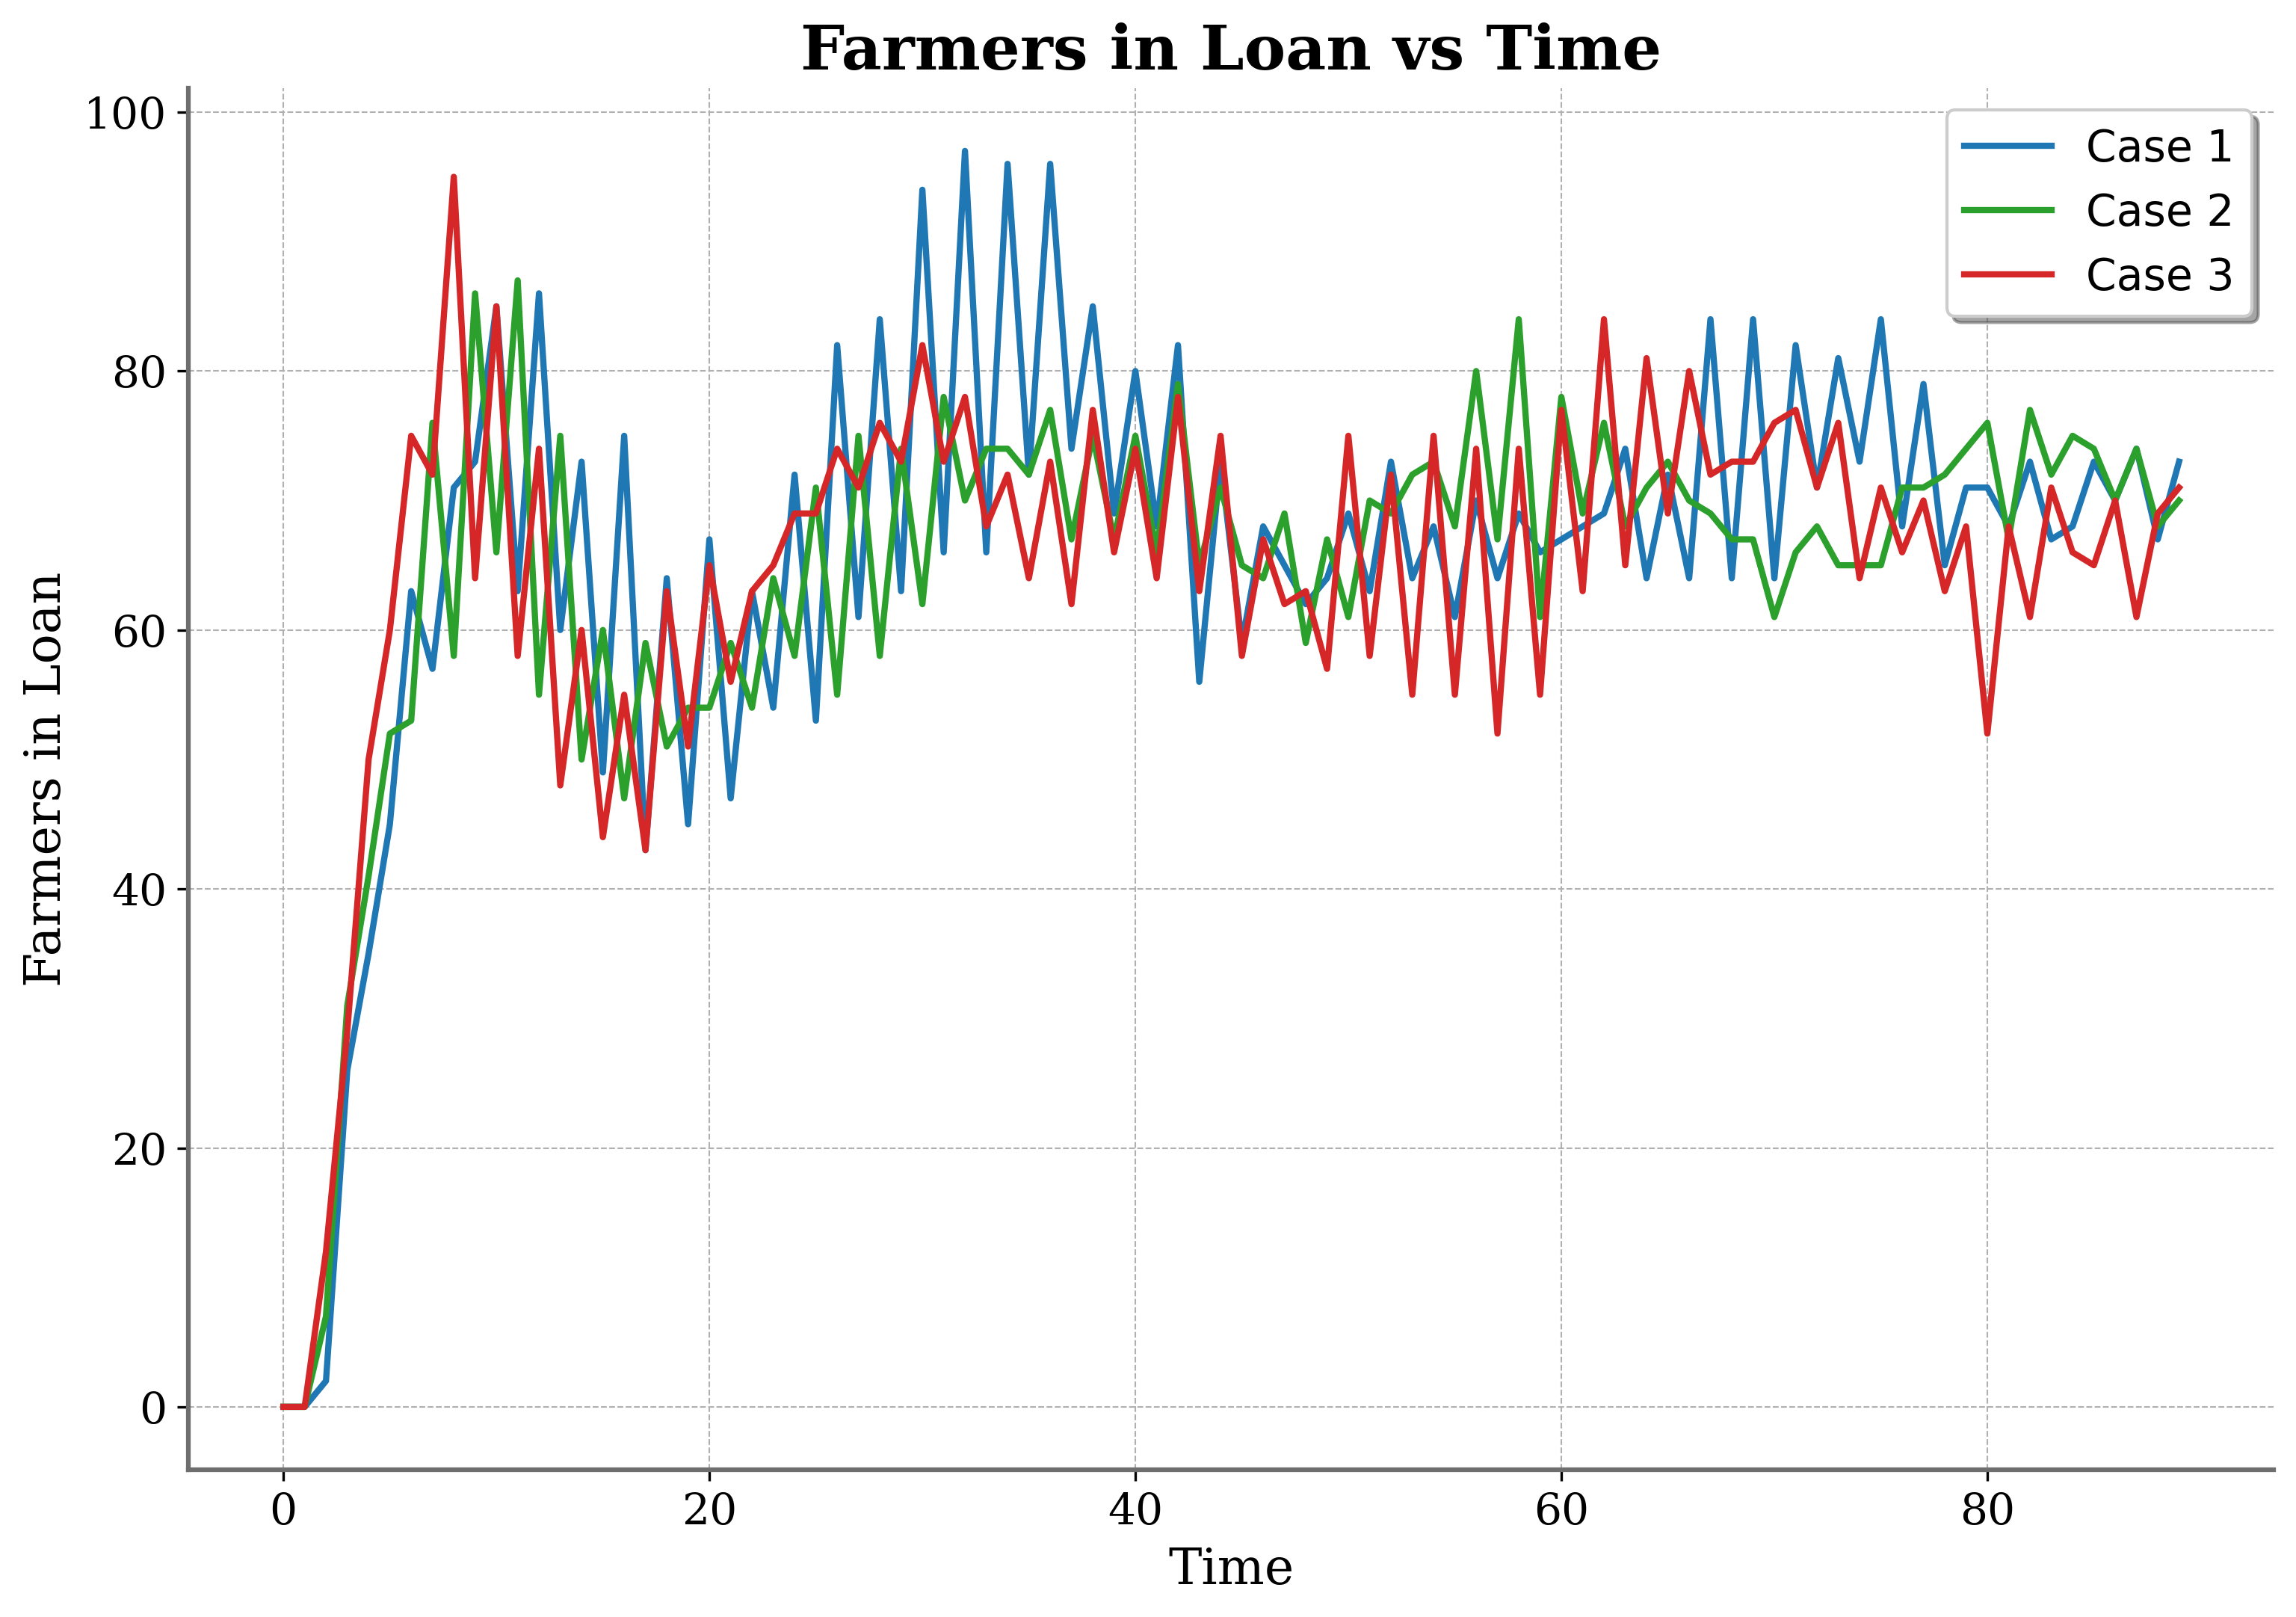
\includegraphics[width=0.4\textwidth]{graph_all/plots_crit/farmers_in_loan_vs_time.png}
    \caption{Farmers in Loan vs Time}
    \label{fig:farmers_loan}
\end{figure}
\begin{table}[htbp]
    \centering
    \resizebox{0.4\textwidth}{!}{ % Adjust the 0.9 to control the table size
    \begin{tabular}{lccc}
        \toprule
        \textbf{Statistic} & \textbf{Case 1} & \textbf{Case 2} & \textbf{Case 3} \\
        \midrule
        Mean & 66.35556 & 64.88889 & 64.81111 \\
        Median & 68 & 68 & 68 \\
        Min & 0 & 0 & 0 \\
        Max & 97 & 87 & 95 \\
        Range & 97 & 87 & 95 \\
        Standard Deviation & 17.23487 & 14.97072 & 15.19824 \\
        Variance & 297.0407 & 224.1223 & 230.9864 \\
        Interquartile Range & 10 & 12.75 & 12.75 \\
        Skewness & -1.8329 & -2.54619 & -2.23415 \\
        Kurtosis & 5.329643 & 8.214303 & 7.016582 \\
        First Quartile & 63 & 61 & 61 \\
        Third Quartile & 73 & 73.75 & 73.75 \\
        MAD & 5 & 6 & 6 \\
        Coefficient of Variation & 0.259735 & 0.230713 & 0.2345 \\
        Mode & 64 & 67 & 63 \\
        \bottomrule
    \end{tabular}
    }
    \caption{Farmers in Loan - Statistical Analysis}
\end{table}
The study reveals that loan involvement among farmers (Figure 20 and Table 20) is fluctuating and precarious in all three scenarios. Case 1 has the highest mean value, with a higher number of farmers involved in loans. Case 1 also exhibits the highest level of variability, with negative skewness values and dramatic fluctuations. The interquartile range and MAD values show a wider spread and larger deviations, indicating more inconsistency. Loan participation is significant in all circumstances, but Case 1 has higher levels of volatility and extremes, suggesting greater uncertainty or stress during crucial conditions. Implementing financial stability measures is crucial to sustain continuous participation in loan programs.\\
% Seventh figure for Crop Production Capacity
\begin{figure}[htbp]
    \centering
    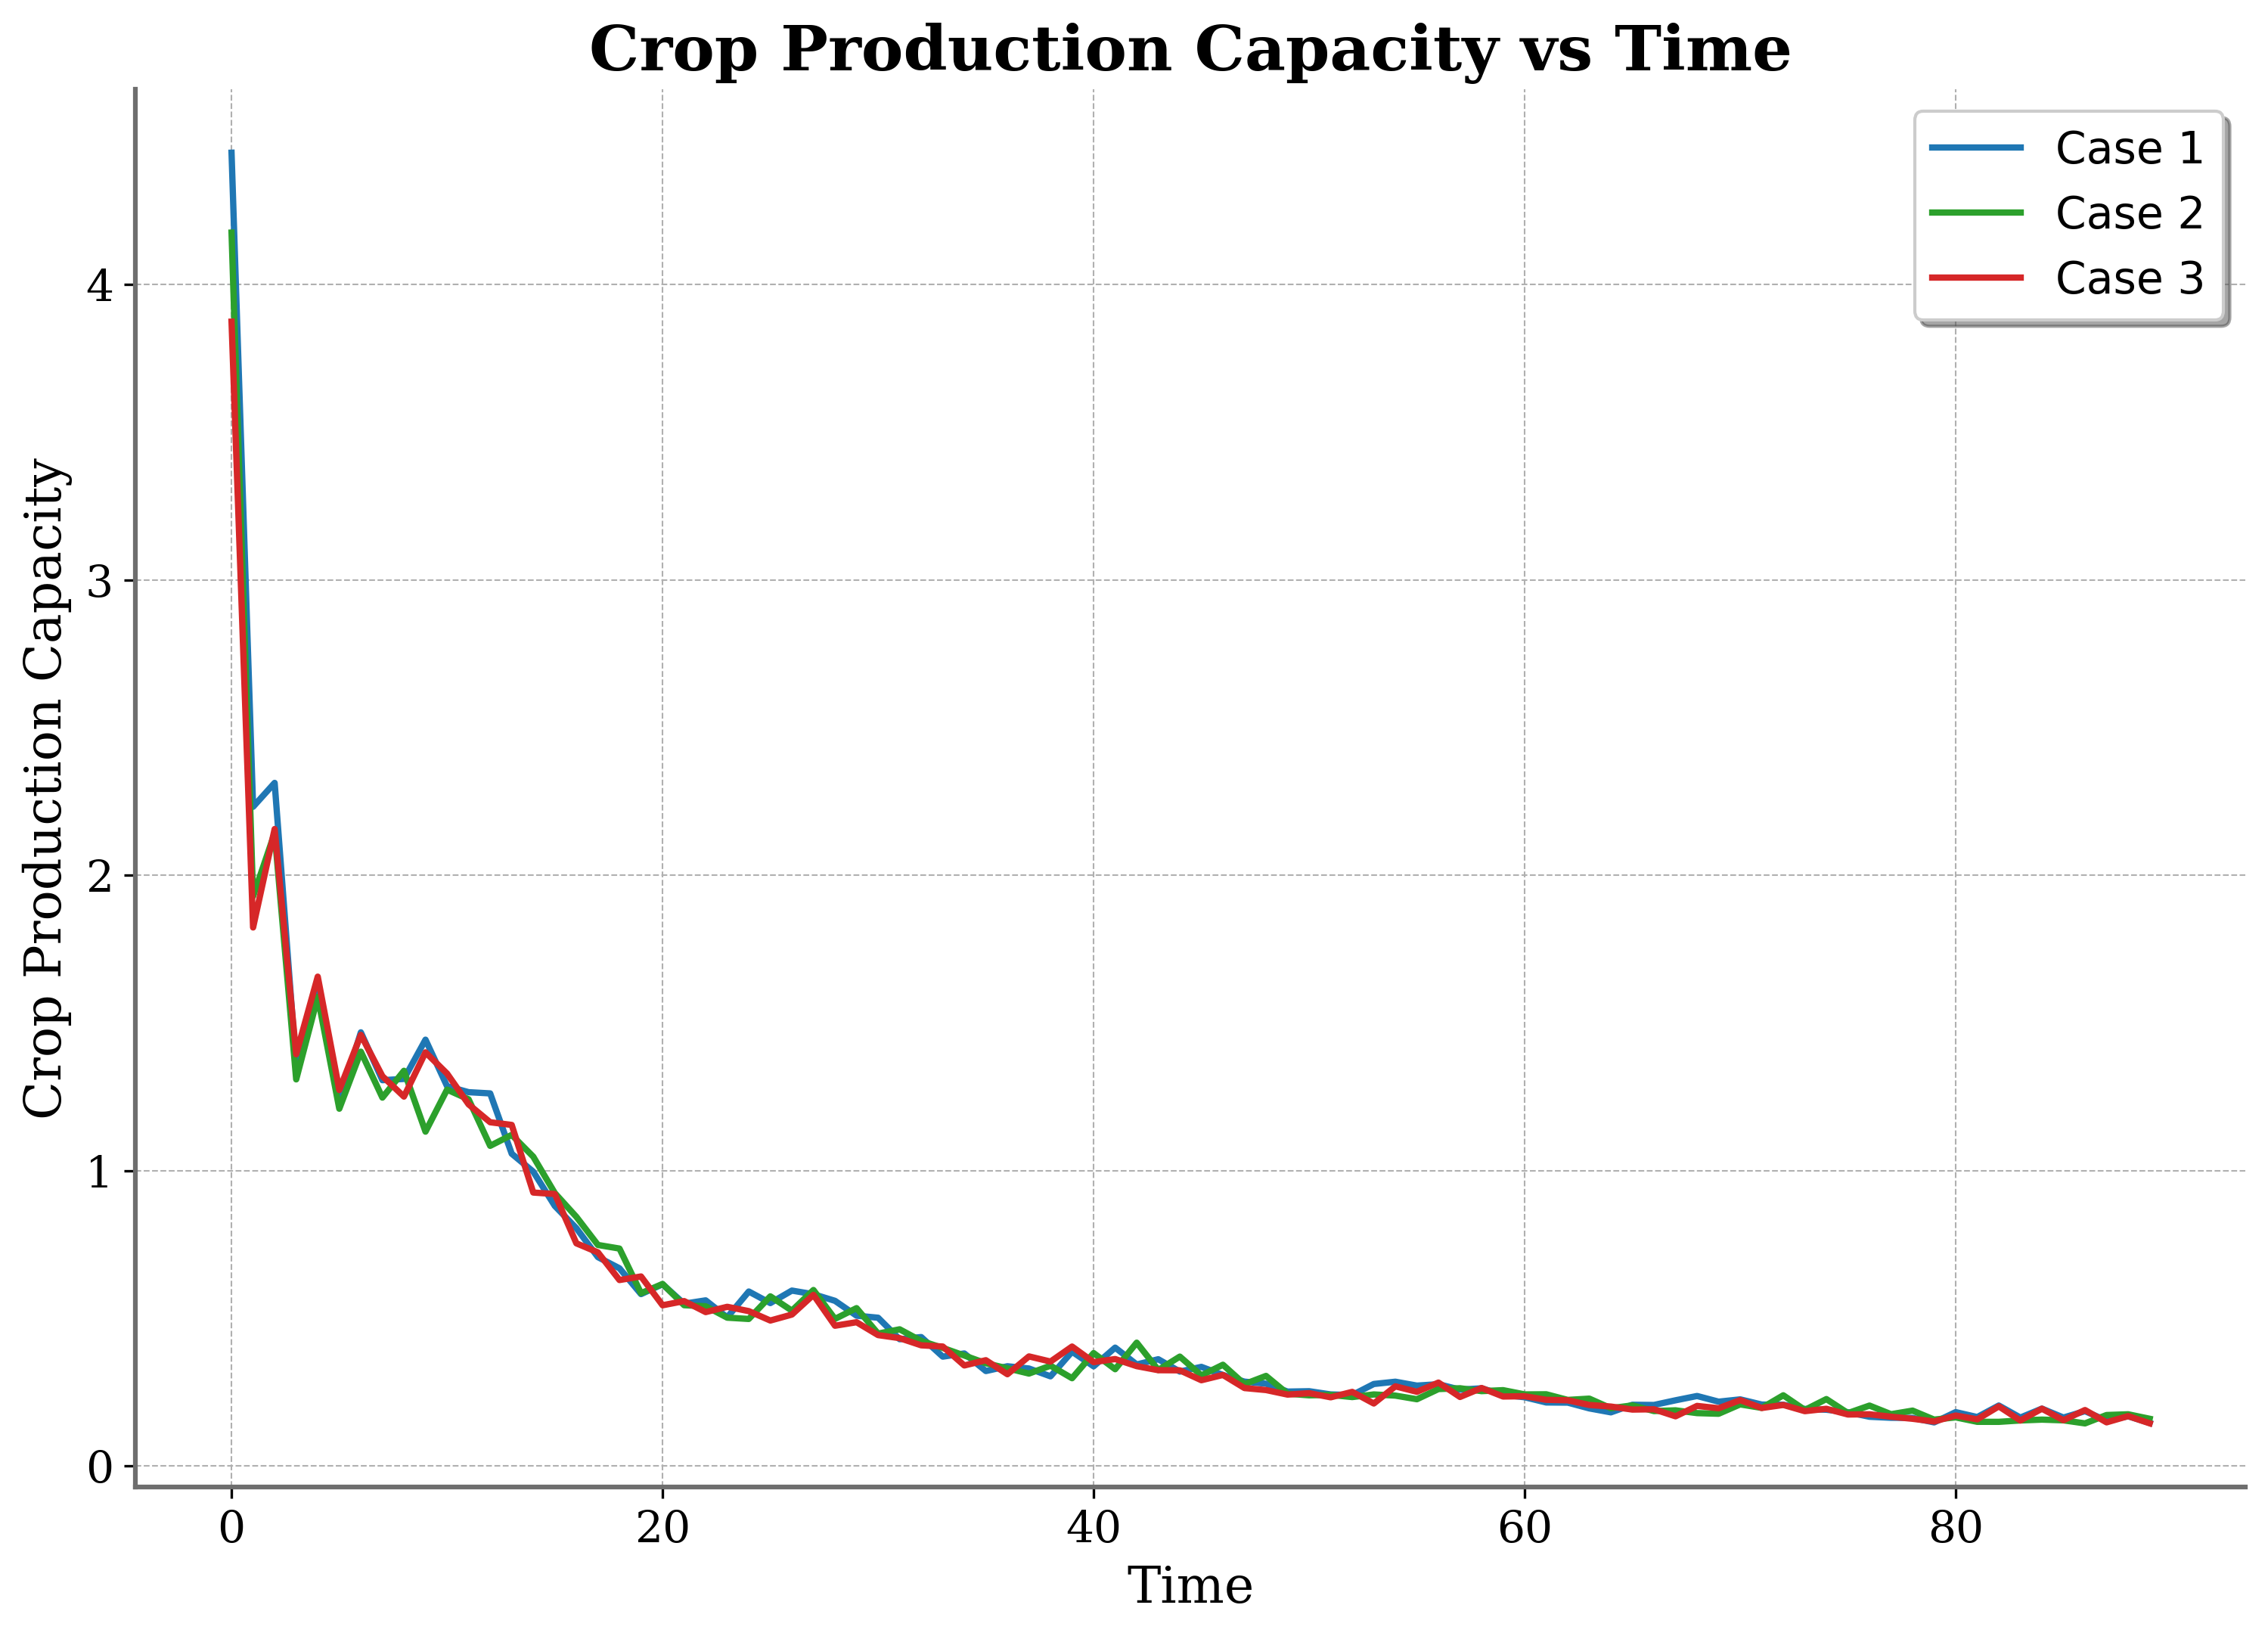
\includegraphics[width=0.4\textwidth]{graph_all/plots_crit/crop_production_capacity_vs_time.png}
    \caption{Crop Production Capacity vs Time}
    \label{fig:crop_production}
\end{figure}
\begin{table}[htbp]
    \centering
    \resizebox{0.4\textwidth}{!}{ % Adjust the 0.9 to control the table size
    \begin{tabular}{lccc}
        \toprule
        \textbf{Statistic} & \textbf{Case 1} & \textbf{Case 2} & \textbf{Case 3} \\
        \midrule
        Mean & 0.547136 & 0.529374 & 0.525139 \\
        Median & 0.314288 & 0.310241 & 0.309803 \\
        Min & 0.146057 & 0.144602 & 0.144885 \\
        Max & 4.446477 & 4.176063 & 3.874559 \\
        Range & 4.30042 & 4.031461 & 3.729673 \\
        Standard Deviation & 0.618583 & 0.578025 & 0.563959 \\
        Variance & 0.382645 & 0.334113 & 0.31805 \\
        Interquartile Range & 0.372231 & 0.36086 & 0.340551 \\
        Skewness & 3.520581 & 3.452459 & 3.0848 \\
        Kurtosis & 16.76236 & 16.5561 & 12.93689 \\
        First Quartile & 0.209973 & 0.206382 & 0.202627 \\
        Third Quartile & 0.582204 & 0.567242 & 0.543177 \\
        MAD & 0.125843 & 0.131931 & 0.123578 \\
        Coefficient of Variation & 1.130585 & 1.091905 & 1.073924 \\
        Mode & 0.146057 & 0.144602 & 0.144885 \\
        \bottomrule
    \end{tabular}
    }
    \caption{Crop Production Capacity - Statistical Analysis}
\end{table}
The analysis of crop production capacity under demanding conditions (Figure 21 and Table 21) shows an initial decrease in capacity, followed by gradual stabilization over time. This pattern aligns with stressors in a critical environment, causing a substantial decrease in crop productivity before stabilizing. Statistically, mean values range from 0.525139 to 0.547136, with the highest standard deviation and variance values in Case 1. The interquartile range is greatest in Case 1, indicating greater variability and worse predictability. The distribution is more positively skewed in Case 1, suggesting instability or susceptibility to maintaining productivity. Effective intervention efforts should aim to decrease variability and promote consistent agricultural yields.\\
\\
By analyzing livelihood agents in favorable, moderate, and critical situations, we identified clear patterns and inequalities, which emphasize how environmental conditions affect various groups. Under optimal circumstances, the majority of agents exhibited consistent and uniform performance, characterized by minimal fluctuations in both temporal patterns and statistical metrics. For example, the narratives of "Golpata Stock" and "Catching Capacity" constantly portrayed pleasant outcomes, suggesting the presence of ample resources and effective administration in advantageous conditions. Nevertheless, when the conditions improved, there was a noticeable rise in the level of variability observed in all instances, marked by more prominent swings and broader ranges between the first and third quartiles. This transformation implies that in difficult circumstances, the availability of resources and the actions of individuals become less reliable, requiring the implementation of flexible methods to ensure stability.

Amidst extremely difficult situations, there was a notable increase in instability across all contexts. The time-series plots exhibited higher levels of volatility, as evidenced by increasing standard deviations and variances, which indicated a greater degree of uncertainty and pressure. The agents known as "Mangrove Fishers in Loan" and "Household Fishers in Loan" had the highest level of sensitivity to unfavorable conditions, as seen by significant decreases and unpredictable patterns of involvement in certain instances. The skewness and kurtosis measurements indicate that the distribution of these cases is skewed towards extreme values and outliers, suggesting a propensity for sudden shifts in behavior or output.

To summarize, the comparative analysis shows that when conditions are favorable, stability and resilience are achieved. However, in intermediate and severe scenarios, significant risks and variability emerge. This highlights the significance of strong support networks, flexible policies, and effective resource management strategies to minimize negative impacts in difficult situations. The findings emphasize the importance of implementing focused interventions in crucial circumstances to guarantee the long-term viability and effective utilization of resources, particularly for susceptible communities like the Bawali and mangrove fishers.
% Force all previous floats to be placed before continuing
\FloatBarrier

% Anik-------------------------------------ekhan theke lekho

\subsection{Effect of Policy Interventions}

We define a policy as a set of conditions and corresponding actions. For a clear presentation of the conditions and actions, we define three variables $ gf, zf, rf $. The definitions of these variables are as follows:


$gf$: The fraction of the initial Golpata stock that is currently present. Therefore,
\[
gf = \frac{\text{current stock of Golpata}}{\text{initial stock of Golpata}}
\]

$zf$: The fraction of Bawalis whose Golpata collection permission will be withdrawn completely. Therefore,
\[
zf = \frac{\text{number of Bawalis with zero permission}}{\text{total number of Bawalis}}
\]

$rf$: The fraction of maximum permitted amount that will be allowed for the rest of the Bawalis. Therefore,
\[
rf = \frac{\text{permitted amount for rest of the Bawalis}}{\text{maximum permitted amount}}
\]

A condition will be denoted as a relational expression involving $gf$ and the corresponding action will be fully described by the pair $(zf, rf)$. To elucidate, if a condition is expressed as $ 0.25 \leq gf < 0.5 $, $zf = 0.1$, and $rf = 0.8$, it means, when the Golpata stock falls between 25\% and 50\% of the initial Golpata stock, 10\% of the Bawalis will be denied the permission completely and the rest of the Bawalis will be permitted an amount that is 80\% of the maximum extraction permission.

\begin{table}[h!]
	\centering
	\scriptsize  % Adjust font size
	\setlength{\tabcolsep}{3pt}  % Reduce column padding
	\renewcommand{\arraystretch}{1.1}  % Adjust row height
	\begin{tabular}{|c|l|c|c|}
		\hline
		\textbf{Name} & \textbf{Condition}                  & \textbf{$zf$} & \textbf{$rf$} \\ \hline
		
		\multirow{1}{*}{Policy 1} 
		& $ gf < 0.25 $ & 0.2 & 0.2  \\ \hline 
		
		\multirow{2}{*}{Policy 2} 
		& $ gf < 0.25 $ & 0.5 & 0.1  \\ \cline{2-4} 
		& $ 0.25 \leq gf < 0.5 $  & 0.1 & 0.8  \\ \hline
		
		\multirow{3}{*}{Policy 3} 
		& $ gf < 0.25 $ & 0.5 & 0.1  \\ \cline{2-4} 
		& $ 0.25 \leq gf < 0.33 $  & 0.3 & 0.5  \\ \cline{2-4}
		& $ 0.33 \leq gf < 0.5 $  & 0.1 & 0.8  \\ \hline
		
	\end{tabular}
	\caption{Definitions of three experimental policies}
	\label{tab:policy_defs}
\end{table}

Table \ref{tab:policy_defs} shows the three policies that we experiment with. The first policy consists only one (condition, action) pair while the third contains three such pairs. 

% Policy figure for Golpata Stock
\begin{figure}[htbp]
	\centering
	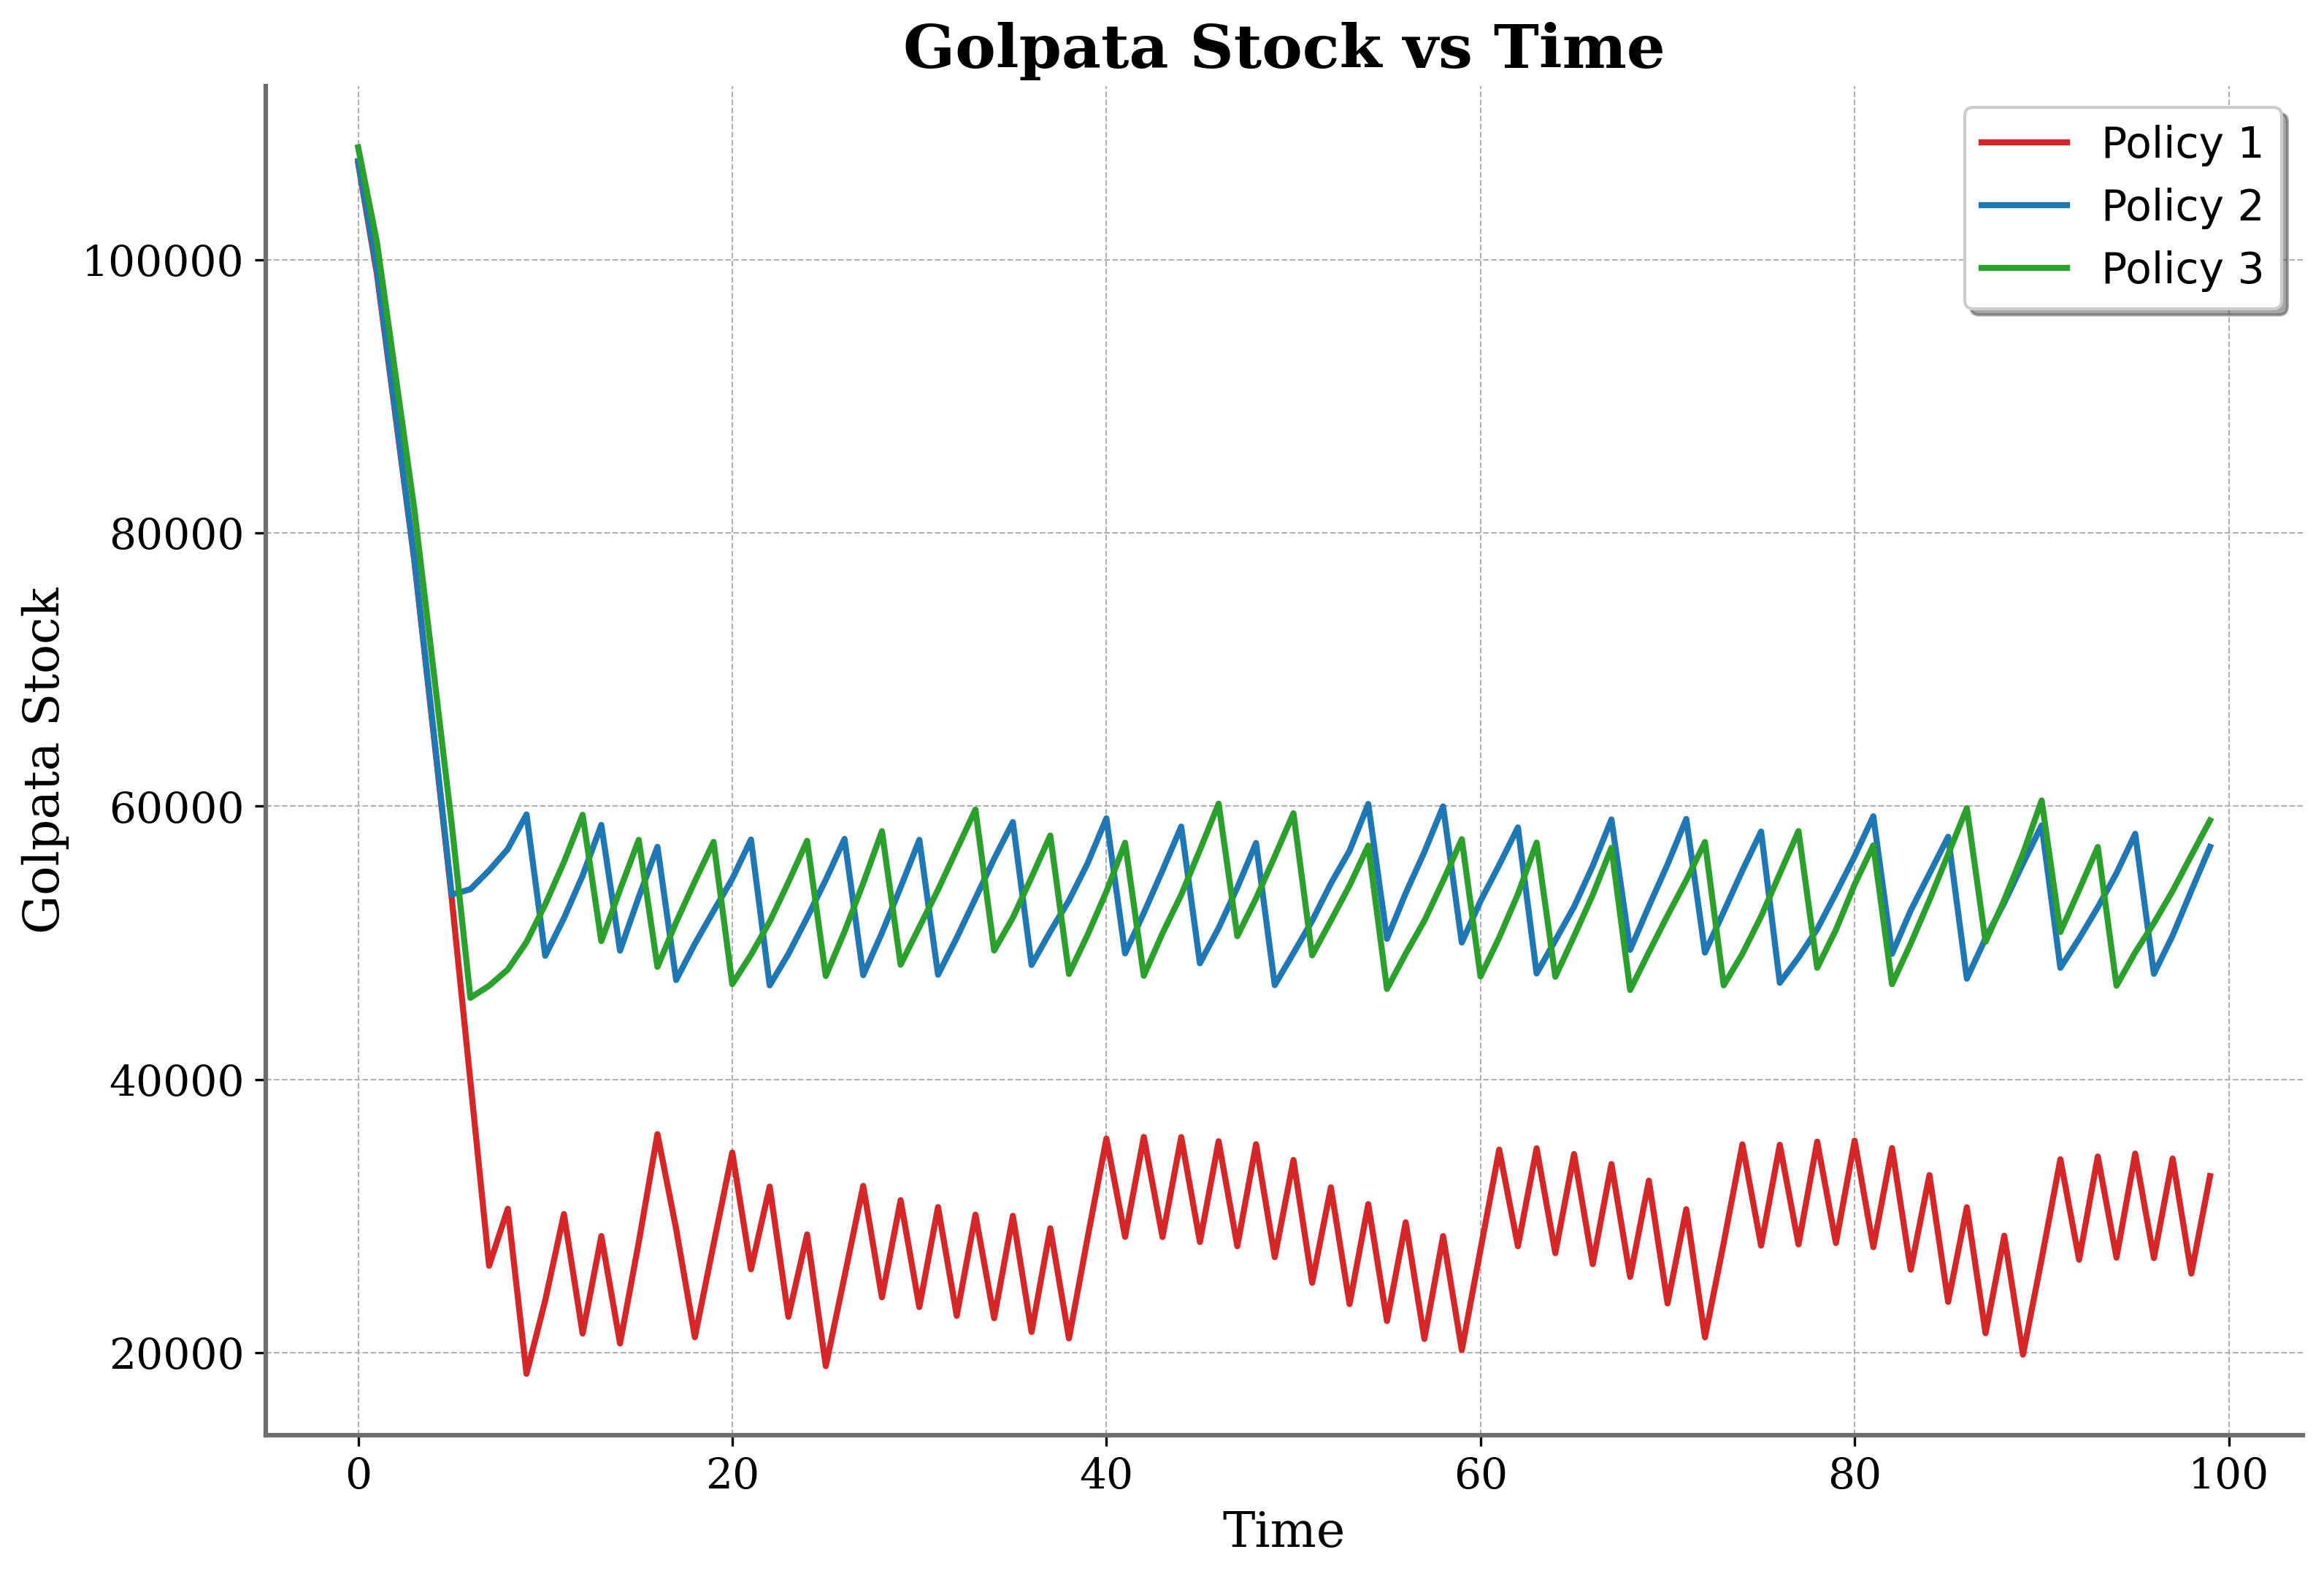
\includegraphics[width=0.4\textwidth]{graph_all/plots_policy/golpata_stock_vs_time.png}
	\caption{Golpata Stock vs Time}
	\label{fig:policy_golpata_stock}
\end{figure}
\begin{table}[htbp]
	\centering
	\resizebox{0.4\textwidth}{!}{ % Adjust the 0.9 to control the table size
		\begin{tabular}{lccc}
			\toprule
			\textbf{Statistic} & \textbf{Policy 1} & \textbf{Policy 2} & \textbf{Policy 3} \\
			\midrule
			
			Mean & 31764.5284 & 55069.707 & 54815.9603\\
			Median & 28488.6069 & 53628.4155 & 53509.6093\\
			Min & 18432.2469 & 46882.7165 & 45967.67\\
			Max & 107099.4772 & 107252.1092 & 108256.1556\\
			Range & 88667.2303 & 60369.3927 & 62288.4856\\
			Standard Deviation & 14363.0782 & 9035.6306 & 9623.9172\\
			Variance & 206298014.507 & 81642619.4709 & 92619782.5804\\
			Interquartile Range (IQR) & 8435.6347 & 6724.1895 & 7018.7999\\
			Skewness & 3.5541 & 3.7602 & 3.6175\\
			Kurtosis & 13.655 & 16.7405 & 15.2296\\
			First Quartile & 25721.5968 & 50299.6642 & 50024.4162\\
			Third Quartile & 34157.2314 & 57023.8538 & 57043.2161\\
			MAD (Mean Absolute Deviation) & 7616.257 & 4921.4391 & 5324.5014\\
			Coefficient of Variation & 0.4522 & 0.1641 & 0.1756\\
			
			\bottomrule
		\end{tabular}
	}
	\caption{Golpata Stock under Different Policies - Statistical Analysis}
	\label{tab:policy_golpata_stock}
\end{table}

From Figure \ref{fig:policy_golpata_stock} and Table \ref{tab:policy_golpata_stock} , it is evident that applying Policy 1 not only reduces the mean Golpata stock but also results in greater fluctuations in the stock over time. The mean amount of stock steadily increases as we shift from Policy 1 towards Policy 3 while the standard deviation decreases in a similar manner. The coefficient of variation drop down to 16.52\% in case of Policy 3 from an alarming rate of 47\% for Policy 1. Although the metrics show an increasing tendency in almost all the cases, it is notable that the metrics observed for Policy 2 and Policy 3 do not vary much from each other, ascertaining the fact that at least two (condition, action) pairs are necessary to be included in the policy for a decent state of the Golpata stock. 

Next, we analyze the effects of policy interventions on the switching of professions.

% Policy figure for Bawali Count
\begin{figure}[htbp]
	\centering
	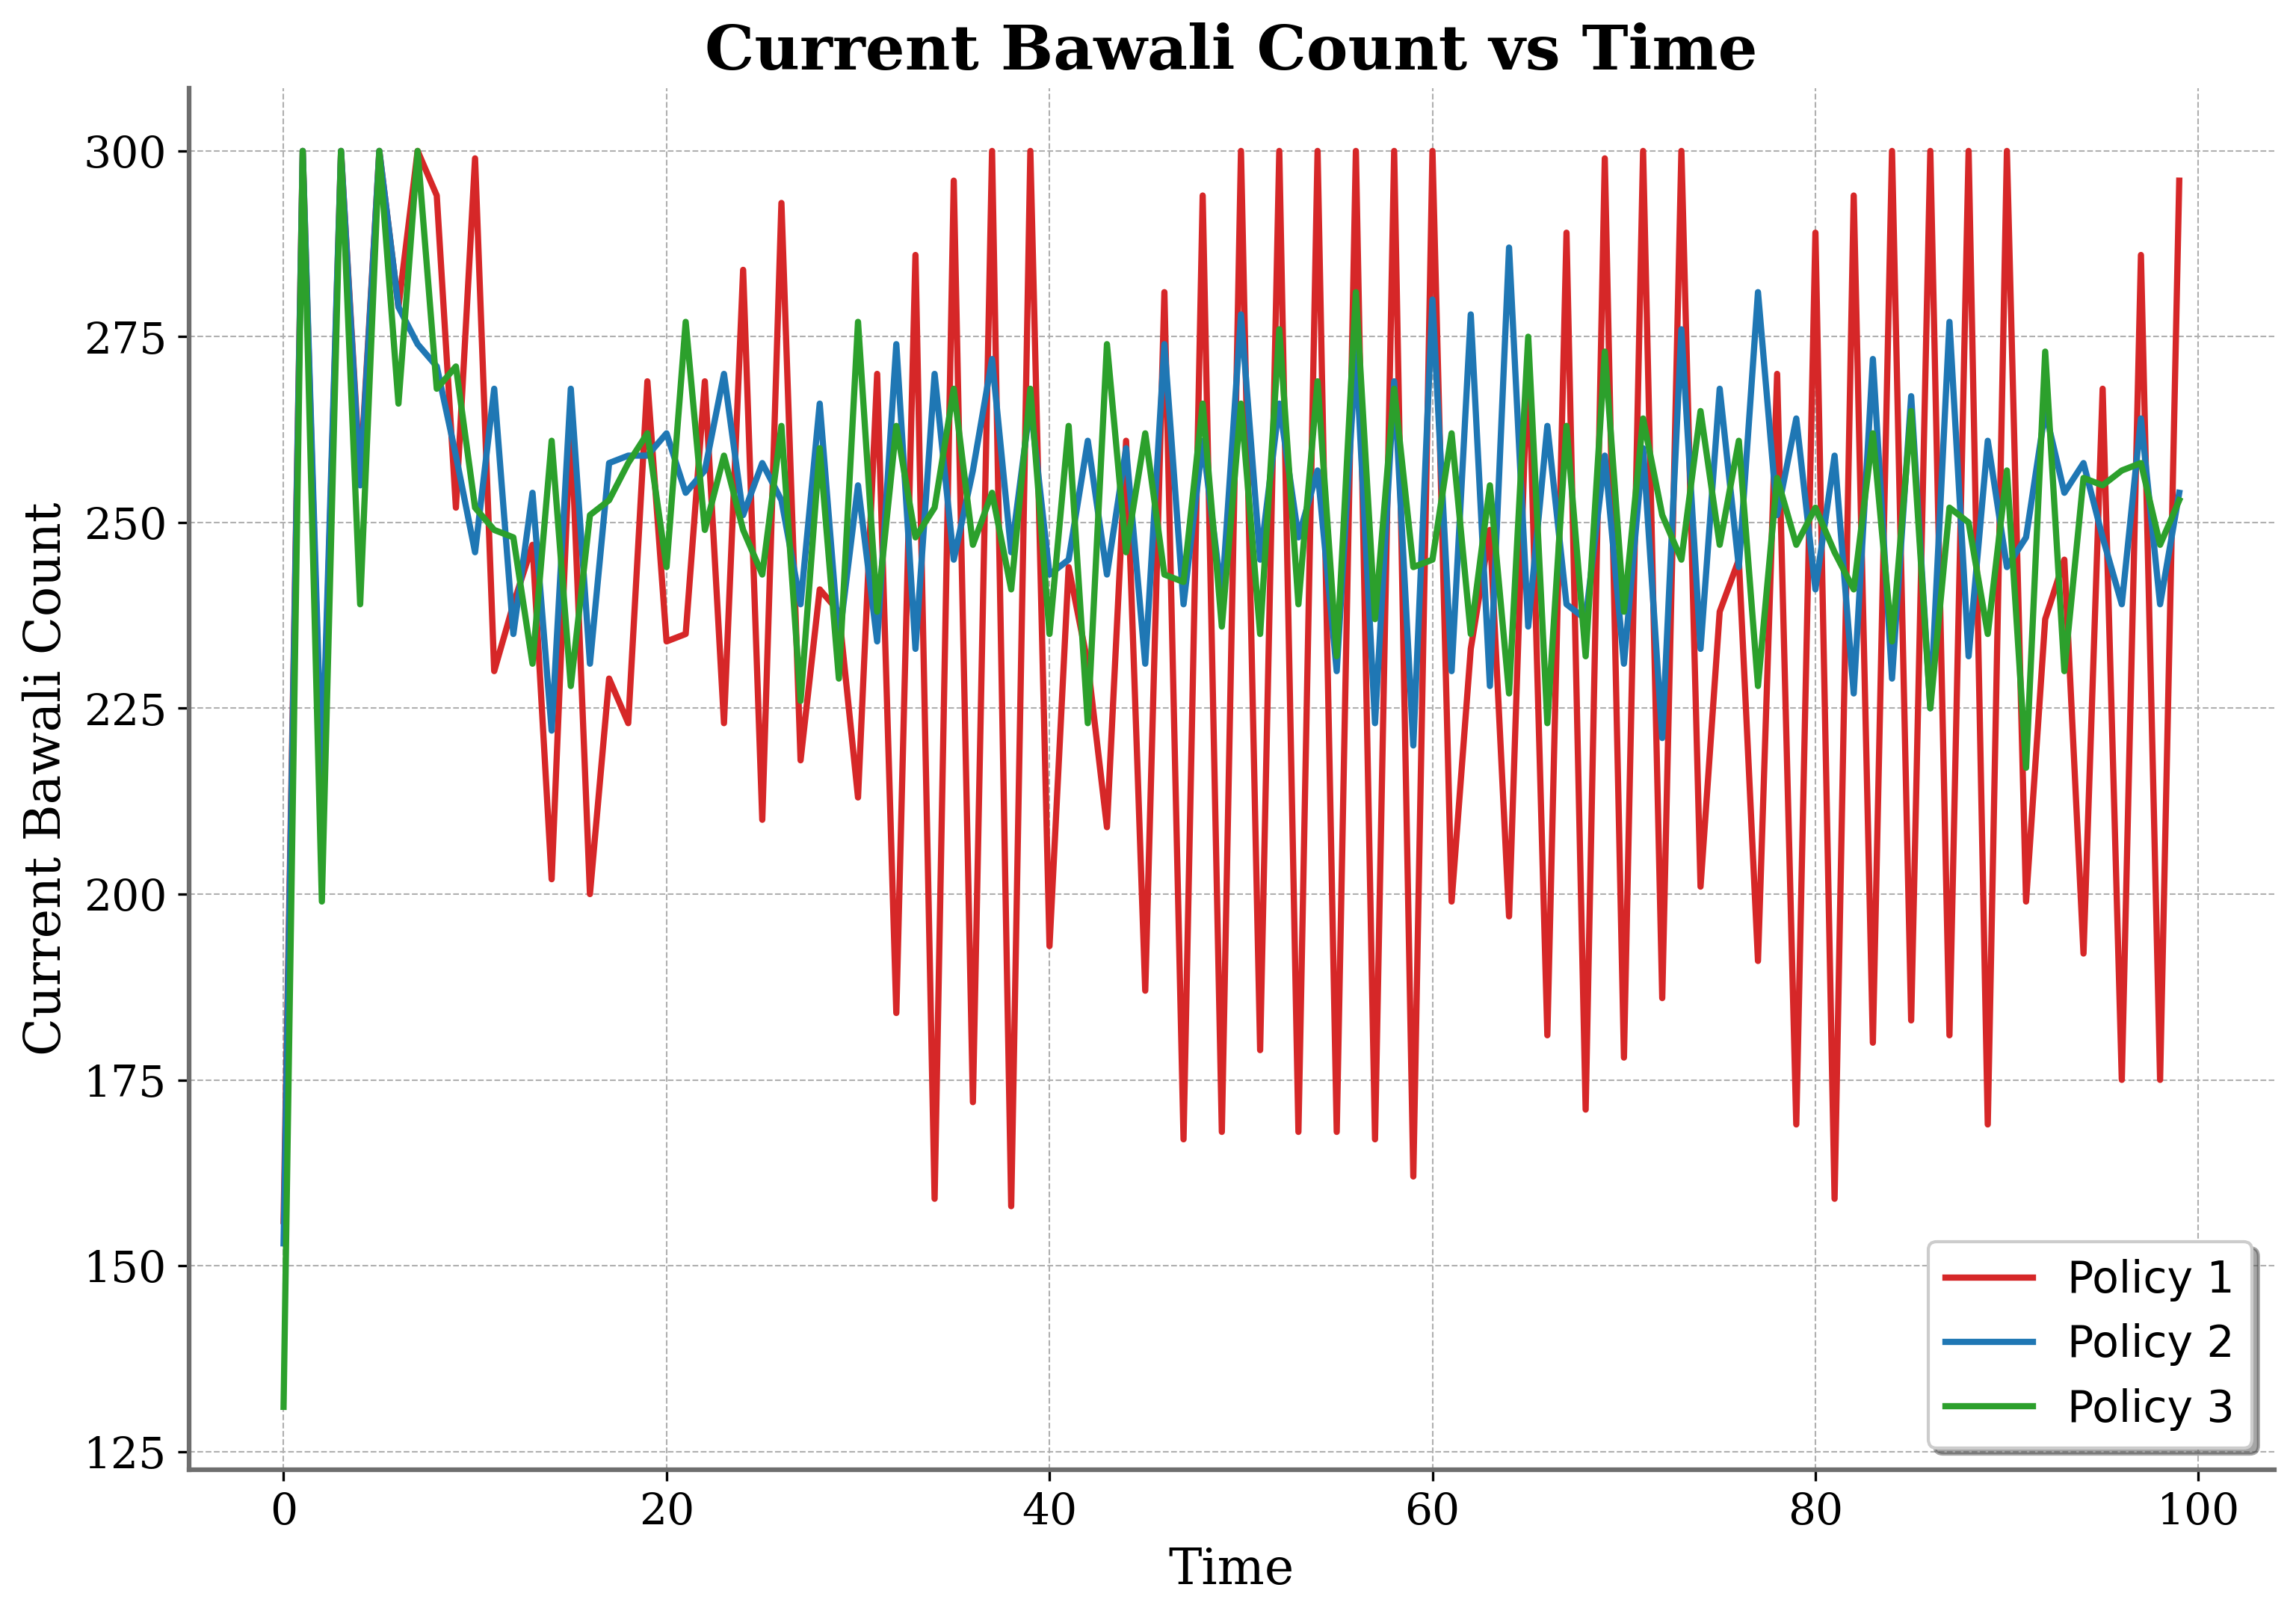
\includegraphics[width=0.4\textwidth]{graph_all/plots_policy/current_bawali_count_vs_time.png}
	\caption{Bawali Count vs Time}
	\label{fig:policy_bawali_count}
\end{figure}
\begin{table}[htbp]
	\centering
	\resizebox{0.4\textwidth}{!}{ % Adjust the 0.9 to control the table size
		\begin{tabular}{lccc}
			\toprule
			\textbf{Statistic} & \textbf{Policy 1} & \textbf{Policy 2} & \textbf{Policy 3} \\
			\midrule
			
			Mean & 238.12 & 252.78 & 251.16\\
			Median & 238.5 & 255.0 & 252.0\\
			Min & 156 & 153 & 131\\
			Max & 300 & 300 & 300\\
			Range & 144 & 147 & 169\\
			Standard Deviation & 50.1811 & 21.0457 & 21.8441\\
			Variance & 2518.1471 & 442.9208 & 477.1661\\
			Interquartile Range (IQR) & 103.25 & 27.25 & 24.0\\
			Skewness & -0.1268 & -0.8539 & -1.4261\\
			Kurtosis & -1.4677 & 3.7716 & 8.1413\\
			First Quartile & 190.0 & 239.0 & 239.0\\
			Third Quartile & 293.25 & 266.25 & 263.0\\
			MAD (Mean Absolute Deviation) & 44.32 & 16.1664 & 15.2368\\
			Coefficient of Variation & 0.2107 & 0.0833 & 0.087\\
			
			\bottomrule
		\end{tabular}
	}
	\caption{Bawali Count under Different Policies - Statistical Analysis}
	\label{tab:policy_golpata_stock}
\end{table}

Figure \ref{fig:policy_bawali_count} further substantiates the volatility arising from the imposition of Policy 1. While the count of Bawalis tends to be turbulent in the case of Policy 1, it proves to be much steadier when we apply Policy 2 and Policy 3. As per Table \ref{fig:policy_bawali_count} the coefficient of variation wanes steeply from 21\% to 8.33\% when we switch from Policy 1 to Policy 2. Since the model assumes that non-rogue Bawalis switch their occupation to Farming when they are denied the permission to extract Golpata, this trend in turn indicates that Policy 1 is enforcing a lot of Bawalis to switch their occupations back and forth while Policy 2 and 3 are offering a greater amount of stability. However, the difference between the effects of Policy 2 and Policy 3 seems negligible as before. In fact, Policy 2 is performing better with respect to some metrics.

Therefore, the results corroborate the notion that policies with greater flexibility and smooth courses of actions perform better than those with stricter actions and single cut-off conditions in terms of maintaining ecological equilibrium.

\subsection{Analyses of Rogue Population}

We investigate the effect of rogue population in case of applying Policy 3, the policy that performed best in terms of stability as per the above results.

% Policy figure for Golpata Stock
\begin{figure}[htbp]
	\centering
	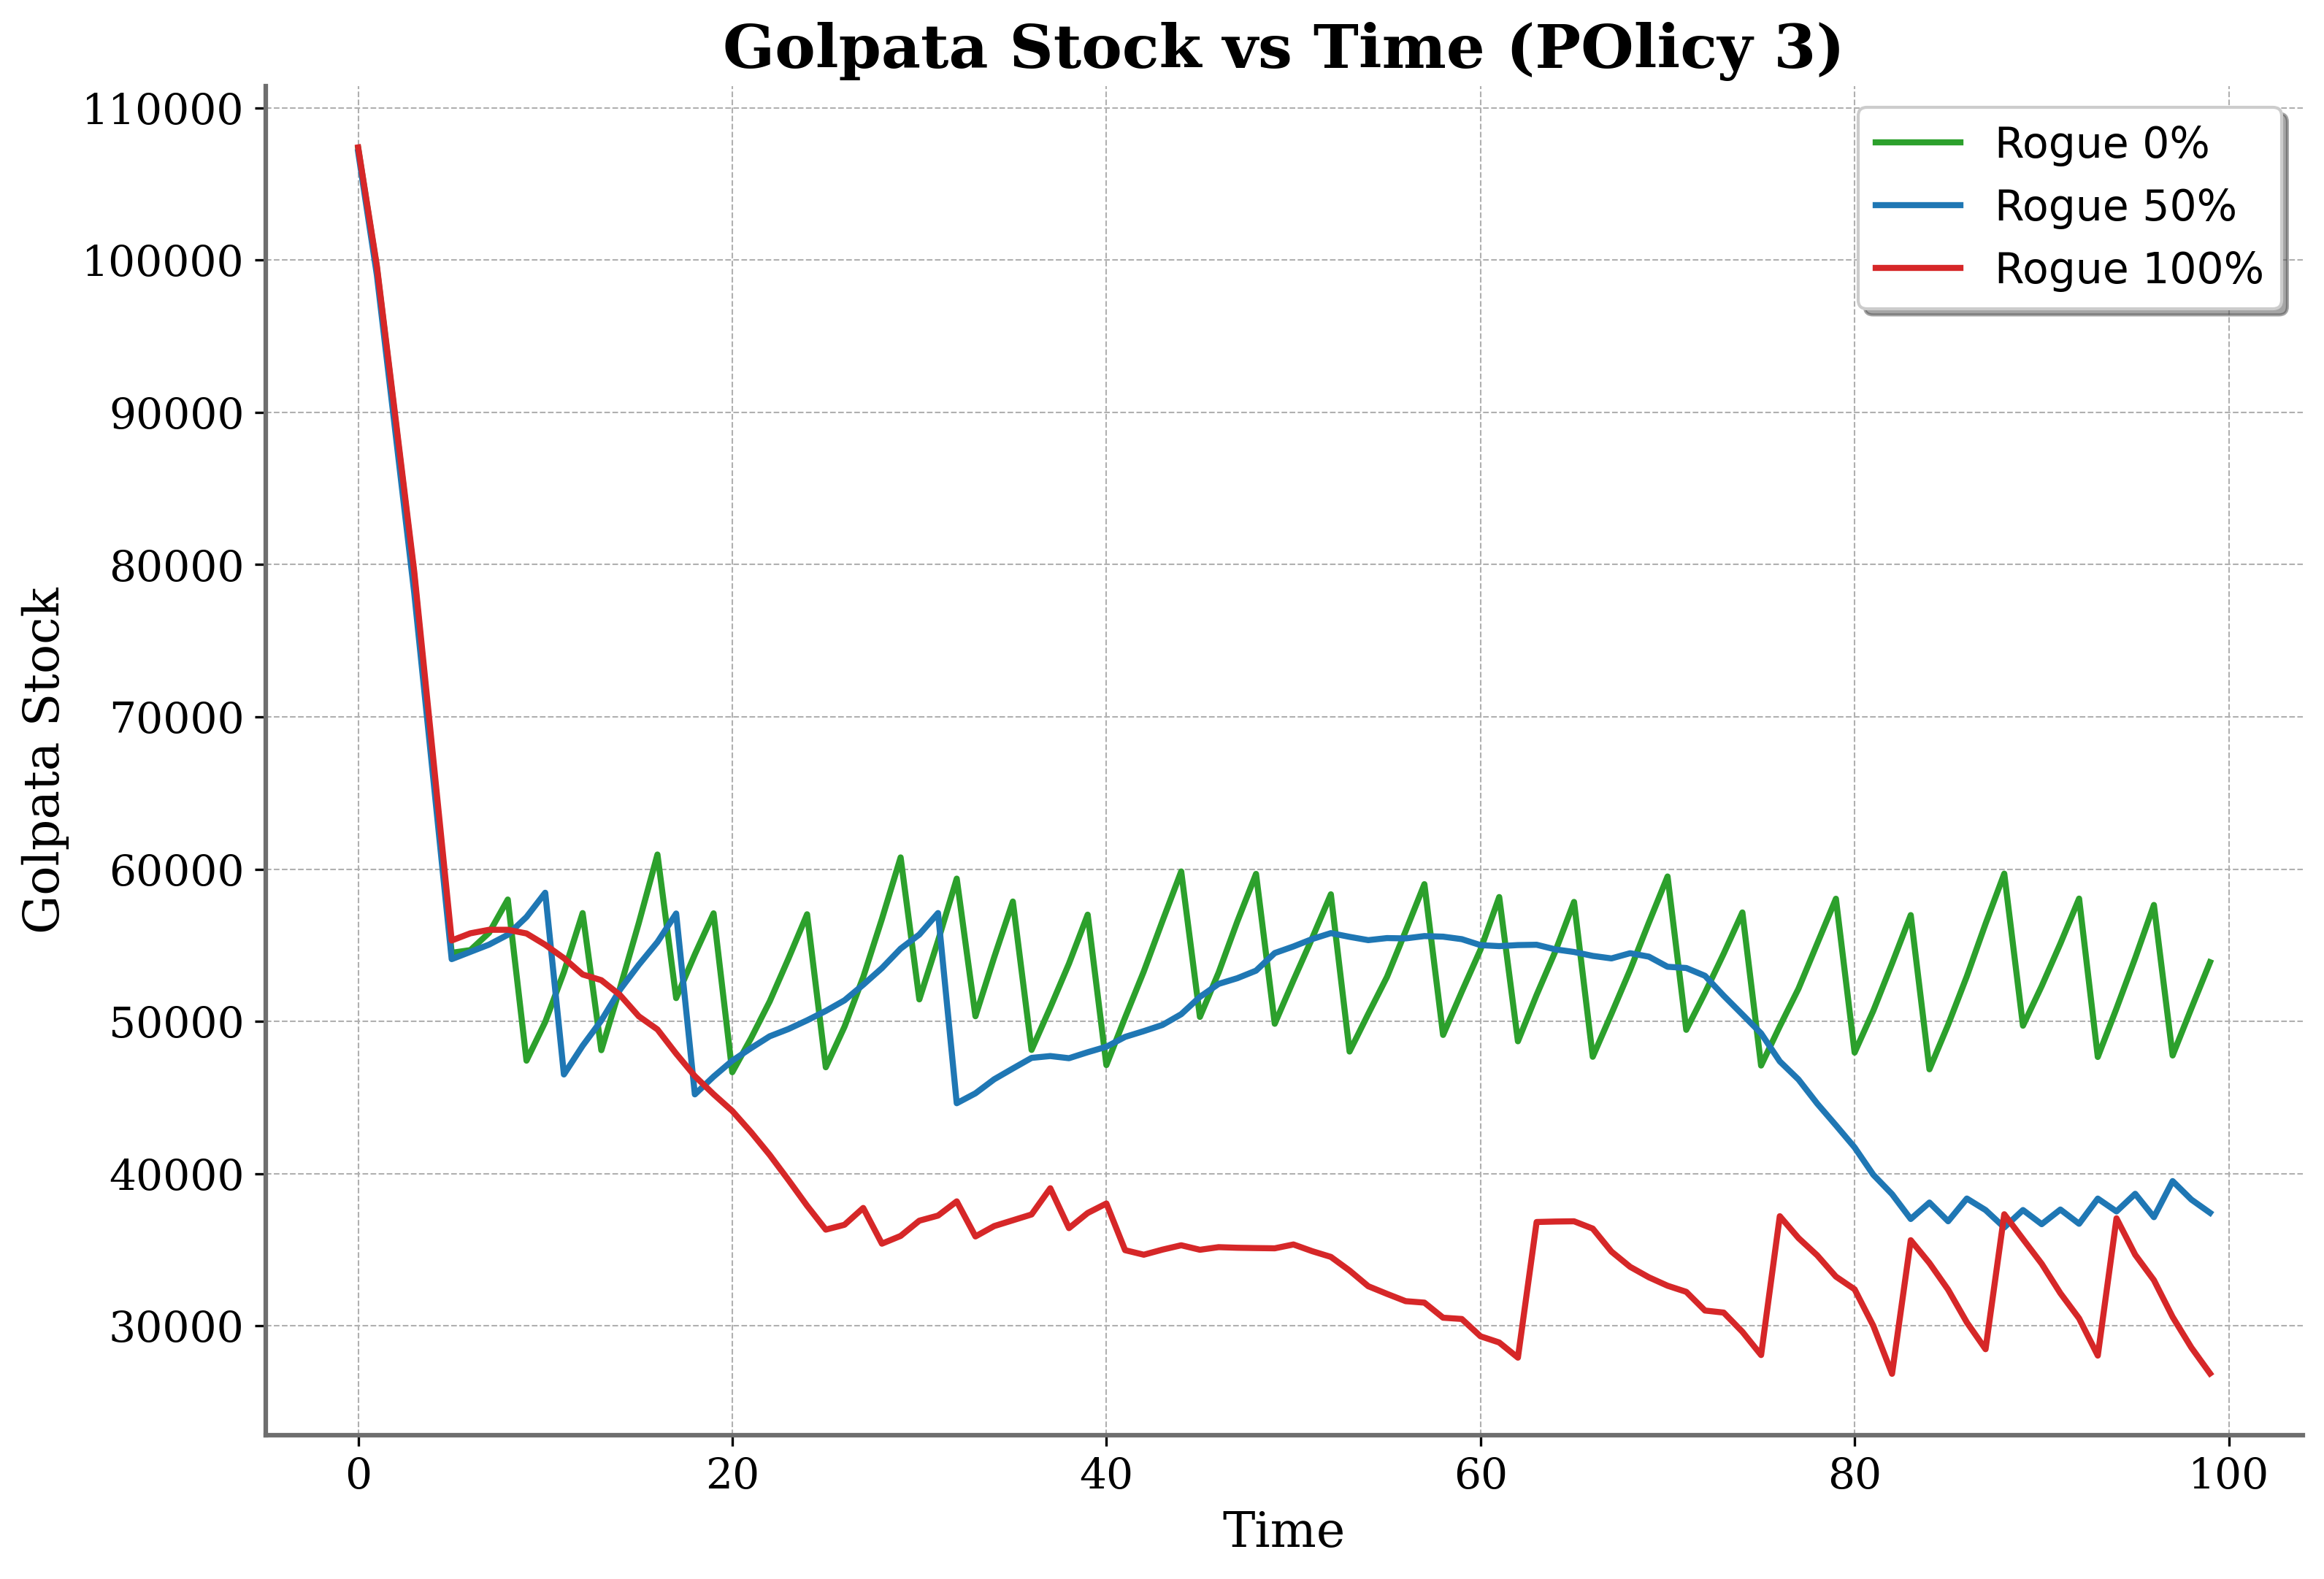
\includegraphics[width=0.4\textwidth]{graph_all/plots_rogue/golpata_stock_vs_time.png}
	\caption{Golpata Stock vs Time (Policy 3)}
	\label{fig:rogue_golpata_stock}
\end{figure}
\begin{table}[htbp]
	\centering
	\resizebox{0.4\textwidth}{!}{ % Adjust the 0.9 to control the table size
		\begin{tabular}{lccc}
			\toprule
			\textbf{Statistic} & \textbf{Rogue 0\%} & \textbf{Rogue 50\%} & \textbf{Rogue 100\%} \\
			\midrule
			
			Mean & 55093.7496 & 50875.708 & 39676.499\\
			Median & 53794.8432 & 51033.1801 & 35513.5949\\
			Min & 46659.5547 & 36465.3213 & 26852.4565\\
			Max & 107345.2114 & 107102.0523 & 107402.189\\
			Range & 60685.6567 & 70636.7311 & 80549.7325\\
			Standard Deviation & 9150.2353 & 11158.8371 & 13841.4524\\
			Variance & 83726805.6787 & 124519646.4361 & 191585803.4079\\       
			Interquartile Range (IQR) & 6689.1282 & 9003.75 & 5839.2925\\      
			Skewness & 3.6949 & 2.3703 & 2.8457\\
			Kurtosis & 16.1524 & 9.2409 & 9.2608\\
			First Quartile & 50325.9716 & 45954.2853 & 32553.7043\\
			Third Quartile & 57015.0998 & 54958.0353 & 38392.9968\\
			MAD (Mean Absolute Deviation) & 5019.5261 & 7005.3166 & 8880.0853\\
			Coefficient of Variation & 0.1661 & 0.2193 & 0.3489\\
			
			\bottomrule
		\end{tabular}
	}
	\caption{Golpata Stock under Different Rogue Rates (Policy 3) - Statistical Analysis}
	\label{tab:rogue_golpata_stock}
\end{table}

Figure \ref{fig:rogue_golpata_stock} and Table \ref{tab:rogue_golpata_stock} delineates the substantial negative impact of rogue population on the ecological balance. The mean Golpata Stock drops by almost 28\% when the percentage of rogue population increases from 0\% to 100\%. Again, the increased coefficient of variation proves the greater amount of instability in case of elevated percentage of rogue population. In the case where half of the population are rogue, the amount seemed to be more stable in the first decades but it eventually dropped down to a more turbulent state in course of time. 

These results emphasize that even if a carefully curated policy is applied, the ecological challenges may still be exacerbated if the percentage of rogue population remains high.




\section{Summary and conclusions}



\section*{Acknowledgements}
Thanks to ...




\printbibliography




\end{document}


